\section{Introduction}

To retain the instructional value of a historical instrument that cannot be played, the kinesthetic actions encoded within the interface must be emulated. Retaining the form of the instrument, such as a commercial MIDI keyboard, is part of achieving successful emulation,\input{articles/context} as will be discussed in Section~\ref{}. 
What is still missing from such keyboards is the haptic information of the instrument, which to \textcite{oboe_mikey_2006}:
\begin{quotation}
    ``allows the player to perceive the ``state'' of the mechanism being manipulated through the key. By using this knowledge about the state of the mechanism and correlating it with the sound generated, the player learns a strategy to obtain desired tones.''
\end{quotation}
The haptics have been passively reintroduced through weighted keys, which attempt to emulate the resistive force of a piano action. Weights do not fully capture the forces at play in piano action, and simplify the full force, including vibrotactile feedback from the acoustic coupling between soundboard and keybed after hammer strikes, the hammer-key and hammer-key impacts, as well as the effect of escapement \cite{oboe_mikey_2006,fluckiger_evaluation_2018}. A major limitation with commercial MIDI interfaces is their reduction of musical expression to simple key attack velocity, of which \textcite{oboe_mikey_2006} writes: 
\begin{quotation}
  ``constitutes a significant limitation for the musician, who loses expressive control of the instrument and, in turn, of the generated sound.''
\end{quotation}
The behaviour of the sound synthesis engine is determined by the speed at which a key moves from its rest position (or central trigger point) to being fully depressed. For the piano, this mapping is quite accurate, since the hammer strike occurs near the bottom of the key’s travel. However, applying the same interface to the harpsichord creates a misrepresentation. This is because most MIDI keyboards trigger their output at the end of the key’s travel, whereas in the harpsichord, both the key’s main haptic and sonic events occur midway through its motion. At that point, the player first feels resistance as the plectrum meets the string, and then again as the jack body presses against the jack rail.

Limited or absent haptic feedback is often framed as a central challenge for
musicians working with synthesisers. Without it, performers are denied the
physical grounding that informs and shapes musical expression. The same absence
of tactile information applies, perhaps even more profoundly, to instruments
that can no longer be played—most notably the fragile musical heritage objects
preserved within museum collections.  

Musical instruments embody a distinctive fusion of form, function, and history.
Their cultural value extends well beyond their visual presence, encompassing
the tactile and auditory dimensions of performance \cite{fritz_listener_2017}.
Yet, in the museum context, preservation demands frequently outweigh these
experiential aspects, restricting direct interaction and reducing instruments
to static artefacts. This ``red velvet cord'' approach
\cite{mcalpine_sampling_2014} safeguards delicate mechanisms but simultaneously
diminishes functional identity, depriving visitors of the full cultural and
historical resonance inherent in these objects.  

The Tagliavini Collection \cite{meer_collezione_2007}, housed at Museo San
Colombano -- Genus Bononiae in Bologna, exemplifies this dilemma. Renowned for
its wealth of historical keyboard instruments—over fifty in total, with a
strong emphasis on Italian plucked stringed keyboards—the collection is a vital
resource for musicologists, organologists, and performers alike. Central to
Ferdinando Tagliavini’s vision was the preservation of authenticity: instruments
were acquired with the specific aim that they might be restored to playing
condition with minimal intervention. Nevertheless, the fragility of their
mechanisms and their historical significance dictate that they are played only
under carefully controlled circumstances, either by experienced historical
keyboard specialists or by students under the close supervision of the curator.  

As part of a broader commitment to accessibility, the Museo San Colombano --
Tagliavini Collection, situated within the cultural itinerary of Fondazione
Carisbo, has undertaken a series of projects designed to improve both cognitive
and sensory engagement. Supported by funding from NextGenerationEU, these
initiatives seek to leverage the collection’s rich holdings to create immersive
and interactive modes of encounter with the exhibited heritage. Central to this
vision is the reinterpretation of historical musical objects through their
tactile and auditory dimensions, with the aim of making the exhibition more
inclusive for blind and partially sighted visitors.  


This initiative led to a collaboration between Museo San Colombano and the NEMUS
project, with the shared goal of creating an interface to digital representations
of historical instruments. The outcome was envisioned as an installation within
the San Colombano exhibition space: a faithful recreation of the haptic
experience of a sixteenth-century Italian harpsichord. At the centre of this
design was an electronically augmented replica, intended to allow visitors to
engage directly with the harpsichord’s distinctive tactile and kinaesthetic
qualities without risk of damage to the original artefacts. Beyond simple
replication, the interface was conceived as an immersive learning environment,
a medium through which the instructional value of the Tagliavini Collection
might be more broadly accessed.  

This chapter documents the development of two such digital musical instruments
(DMIs), beginning with the motivations, constraints, and methodological
framework. Subsequent sections trace the design process in chronological order,
from the earliest prototypes to the full-scale realisation of the concept. The
resulting keyboards reproduce the haptic responses characteristic of an
original fifteenth-century harpsichord, featuring two 8-foot registers typical
of the Italian style \cite{tagliavini_clavicembali_1987}. In doing so, the work
builds on prior explorations in musical heritage
\cite{mcalpine_sampling_2014,baldwin_tromba_2016} as well as four decades of
research into haptic keyboard design.  

In addition to enhancing the visitor experience within the musical instrument
museum, the project engages with a parallel concern: the sustainability of
digital research. The optical sensing technique implemented for the keyboard
adapts earlier work by McPherson on the piano
\cite{mcpherson_portable_2013}. By extending and recontextualising this method,
the project ensures that its outcomes endure beyond their immediate scope,
aligning with best practices for digital research archiving
\cite{smith_software_2016} and addressing long-term considerations for digital
musical instruments (DMIs) and electronics hardware
\cite{mcpherson_nimehub_2016,fiordelmondo_longevity_2024}. The final design
iteration is therefore positioned not only as a practical interface for public
engagement, but also as a research probe: a tool to explore the unique
characteristics of the harpsichord and their implications for musical
performance.  


\section{Related Work and Motivations}\label{related-work}

% Technological advances have transformed how museums document, present and
% interpret their collections. 
% These technologies form a kind of experiential authenticity, enabling encounters
% that evoke the past's sensory, emotional, and intellectual essence
% \cite{trant_when_1999}. \textcite{pine_museums_2007} note, achieving authenticity requires museums to navigat the delicate balance between preservation and meaningful engagement—a challenge
% that is particularly evident in the case of historical musical instrument
% collections \cite{mcalpine_sampling_2014}.

Museums consistently navigate the competing demands of accessibility and
preservation, which restricts the ways in which audiences can interact with
collections \cite{templeton_museum_2018, mcalpine_sampling_2014}. 
For musical instrument museums, these challenges are compounded by the 
difficult choice of maintaining, restoring or preserving the instruments in their collections \cite{barclay_critical_1999,barclay_preservation_2005}. 
For an instrument such as the harpsichord, the nature of its construction means that it is destined to decay, terminating at a
state where it is no longer playable. This is true, even when collections adhere to the
strictest conservation protocols \cite{paradiso_to-save_2019}. In response,
recent decades have witnessed a cultural shift: emphasis has moved away from
playability toward conservation. Karp \cite{karp_restoration_1979, karp_musical_1985} argues for cultivating a deep understanding of musical instruments to generate sufficient knowledge to make
them as ``copyable'' as possible. Not all instruments can be copied, and there is then a choice to be made for which instruments are deserving of recreation. 

With digital instruments, the interface is decoupled from the acoustic sound generator, and the interface can be one-to-many. Communication with various digital heritage instruments can be achieved through a single interface, an approach adopted by \textcite{mcalpine_sampling_2014}. In a case similar to the Tagliavini collection, \textcite{mcalpine_sampling_2014} involved an
examination of the Benton Fletcher Collection at National Trust Fenton House
\cite{mcalpine_sampling_2014}. When these instruments were donated, Benton
Fletcher stipulated that they remain playable and should continue to be
maintained for tuition and public performance. A large sampling campaign was
conducted, and a custom MIDI interface was designed to fulfil this requirement
while preserving the original instruments' integrity. The MIDI controller,
comprising two commercially available keyboards mimicking the two-manual
harpsichord layout, was used by visitors to trigger the instrument samples
recorded with tailored strategies for each. However, user tests identified a
limitation: the commercially available weighted keys failed to provide an
authentic sense of interacting with a historical plucked keyboard instrument
\cite{mcalpine_sampling_2014}. 

The limitations of synthetic interfaces is known limitation of DMI \textcite{magnusson_survey_2007}. The ``Tromba Moderna'' project by \textcite{baldwin_tromba_2016} faced a similar problem to \textcite{mcalpine_sampling_2014}, but strived towards what \textcite{cook_remutualizing_2004} would call ``remutualising'' the interface. \textcite{baldwin_tromba_2016} created the Tromba Moderna for an exhibition at the Musikmuseet Musical Instrument Museum in Copenhagen and the exhibition was to address the problem of engagement and interactivity for visitors to the collection. In this case, the issue of musical heritage playability was approached by recreating and augmenting a replica of a historical tromba marina. A piezo transducer was connected to a sound synthesis engine and a driver within the instrument, and by doing so simulated the expected vibrations of a historical tromba marina. 

The interface described in this chapter builds on these precedents, inheriting
elements from the Tromba Moderna while seeking to extend their scope. Its
design is motivated by the desire to enrich the visitor experience of the
Tagliavini collection, while maintaining continuity with historical
instrument-building traditions. In this sense, both the Tromba Moderna
\cite{baldwin_tromba_2016} and McAlpine’s Benton Fletcher project
\cite{mcalpine_sampling_2014} serve as points of departure. Furthermore, the
development of the harpsichord interface draws on four decades of haptic
keyboard research, embedding this project within a broader lineage of
instrumental interface design.

\subsection{Haptic Keyboards}

To better contextualise the methodology for the project, this section gives a brief timeline of haptic keyboard projects, the modern history of which could be said to begin with 
\textcite{cadoz_synthese_1981}. In under ten years the work of \textcite{cadoz_synthese_1981} was dramatically reduced in size. \textcite{cadoz_modular_1990} feedback keyboard used an array of polarisation magnets and flat coils to introduce a ``tactilo-proprio-kinest'' element to a to a keyboard interface. No photographs of the system are presented, but the figures suggest a large scale and heavy instrument. At a similar time.

Motivations behind these designs were for modular haptic interfaces \cite{cadoz_modular_1990} that could function haptically as more than one type of mechanism. Or the drive was for  by Teleoperation and interaction with virtuals worlds or augmented reality.

\textcite{gillespie_dynamical_1992} created a single haptic-key setup using a linear motor, later refining the concept and simplifying the numerical model \cite{gillespie_virtual_1994}. 
In \textcite{gillespie_virtual_1994} motivation was towards emulation and recapturing the haptical element of performance, a goal emphasised further in the MIKEY (Multi-Instrument active KEYboard) project. MIKEY is a multi-modal haptic interface for replicating the grand piano, harpsichord and hammond organ and can be viewed as drawing from the combined motivations of \textcite{cadoz_modular_1990} and \textcite{gillespie_virtual_1994}.

This was then followed by a single piano key by \textcite{lozada_novel_2007} with haptic feedback enabled through the use of magneto-rheological (MR) fluids. The mechanics of \textcite{lozada_novel_2007} are similar to those of \textcite{cadoz_modular_1990}. 
\textcite{hwang_airpiano_2017} ultrasonic haptics combined with a virtual reality headset and environment. Noted limitation of polyphonic playing.
\textcite{timmermans_multibody-based_2020} further extending concepts \textcite{oboe_mikey_2006}  noting also the benefit that ``key physical characteristics are preserved'' and notably achieving a haptic device with the use of simple, low-cost electronics.

One commonality across all of these projects is that they are typically restricted a single or a small number of keys. For the museum exhibition, the interface would have to be between 38 to 53 keys to match the layouts of the harpsichords in the collection \cite{tagliavini_clavicembali_1987}. The methodologies of the work above were used as basis for the prototyping process. Where this project  diverged from previous work was in an aesthetics-first, rather than technology-first, approach to design. The electronics were hidden inside the interface were not intended to augment or 
disrupt the haptic feedback; rather, they serve as to facilitate a link between the
mechanical and the digital realms as transparently as possible. 

\subsubsection{Visual Aesthetics}

The aesthetics of the instrument well careful considered during the design process.
The physical and visual presentation of an instrument might not be the priority for a performer, but in the context of a museum exhibition it is vital to the visitor experience as demonstrated by \textcite{mcalpine_sampling_2014}.
Since the Tagliavini collection hosts primarily early plucked stringed keyboards of Italian origin,
the keyboard layout was deliberately modelled after early Italian harpsichords.

Often for haptic DMI projects, much of the effort is placed into the design and functionality of electronic components but not much is done with respect to the visual stimulus. 
% Outside of commercial haptic keyboard projects like the vibrotactile AvantGrande series of piano models \cite{fluckiger_evaluation_2018,fluckiger_influence_2018}. Being commercial, its mechanics and software is closed source.
For keyboards, this is in part down to the small number of key modelling \cite{gillespie_haptic_1996,lozada_modelisations_2007,timmermans_multibody-based_2020}, the form of which is already far removed from what a performer would expect. For actuated haptic systems, there is also a question of where to put everything. A combined approach of realistic haptics and aesthetics presents a challenge in design. What differentiates a commercial MIDI keyboard from an acoustic keyboard instrument is the presence of strings. The strings in the interfaces presented here are functional, which is to say their presence serves a purpose as part of both the haptic feedback and visual presentation. If the strings were no longer needed as part of the haptic mechanism, it could be argued their presence would would be necessitate for the purpose of presentation, otherwise what would differentiate the interface visually from current commercial offerings. This then raises the question: where do the electronics go? Haptic systems and electronic actuators have a lower limit for their footprint and often require moving out of the confines of the instrument \cite{mcpherson_augmented_2010, schmidt_sparksichord_2025}.

The impact of visual stimulus should not be underplayed, in particular when it comes to musicians.
The studies of \textcite{fritz_player_2012, fritz_soloist_2014, fritz_listener_2017} covered briefly in Section~\ref{sec:reproduction-or-renovation} illustrates the need for restriction in visual stimulus to avoid influencing a musician when they are listening.
\textcite{tsay_sight_2013} also discusses the impact of quality assessment by ``novices and experts'' alike. In all of those studies, the influence of the visual stimulus was something to be avoided.
This phenomenon, akin to a `musical instrument McGurk effect’ \cite{mcgurk_hearing_1976}, is one of the reasons why the electronics have been concealed from view. 

The McGurk effect is perhaps an apt example. The effect manifests as aural hallucination, typically demonstrated by playing two video each of which shows a mouth, one annunciating the syllable ``ba'' and the other the syllable ``fa'' \cite{horizon_seeing_2010}. The audio synchronised with the videos is always the syllable ``ba'', but typically the sound heard depends on which mouth movment is being observed. The effect is proposed to extend beyond speech and into the domain of visual musical cues \cite{saidana_mcgurk_1990}. The potency of the McGurk effect, particularly as it pertains to musicians has been the subject of debate for the past 30 years. \textcite{proverbio_skilled_2016} and \textcite{alsius_forty_2018} assert that musicians are not as susceptible to the McGurk effect. By contrast, \textcite{politzer_mcgurk_2019} refutes the claim by \textcite{proverbio_skilled_2016} and concludes that not only are musicians as susceptible to non-musicians they are perhaps even more so. The conclusions of \textcite{politzer_mcgurk_2019} when taken alongside \textcite{tsay_sight_2013, fritz_player_2012, fritz_soloist_2014, fritz_listener_2017} show that visual stimulus has non-negligible influence on auditory perception.

Instead of trying to mitigate this influence, the design embraces it and attempts to leverage it. 
Given the extensive research into modelling and recreating piano
action \cite{cadoz_modular_1990, gillespie_haptic_1996, lozada_modelisations_2007,
timmermans_multibody-based_2020}, the visual component may provide the final
persuasive element necessary for acceptance, similar to the way visual
perception affects judgments of musical performance.
The aesthetics of the interface enhance its likelihood of being perceived as an `authentic' musical
instrument. The aesthetic design develops what was observed by \textcite{mcalpine_sampling_2014} and provides a means to answer to what degree can visual stimuli be leveraged to ``sell'' the experience of playing a DMI. When combined with a passive haptic response, are aesthetics enough to influence the player and remove the barrier to convincing experience?

% \begin{figure}
%     \centering
%     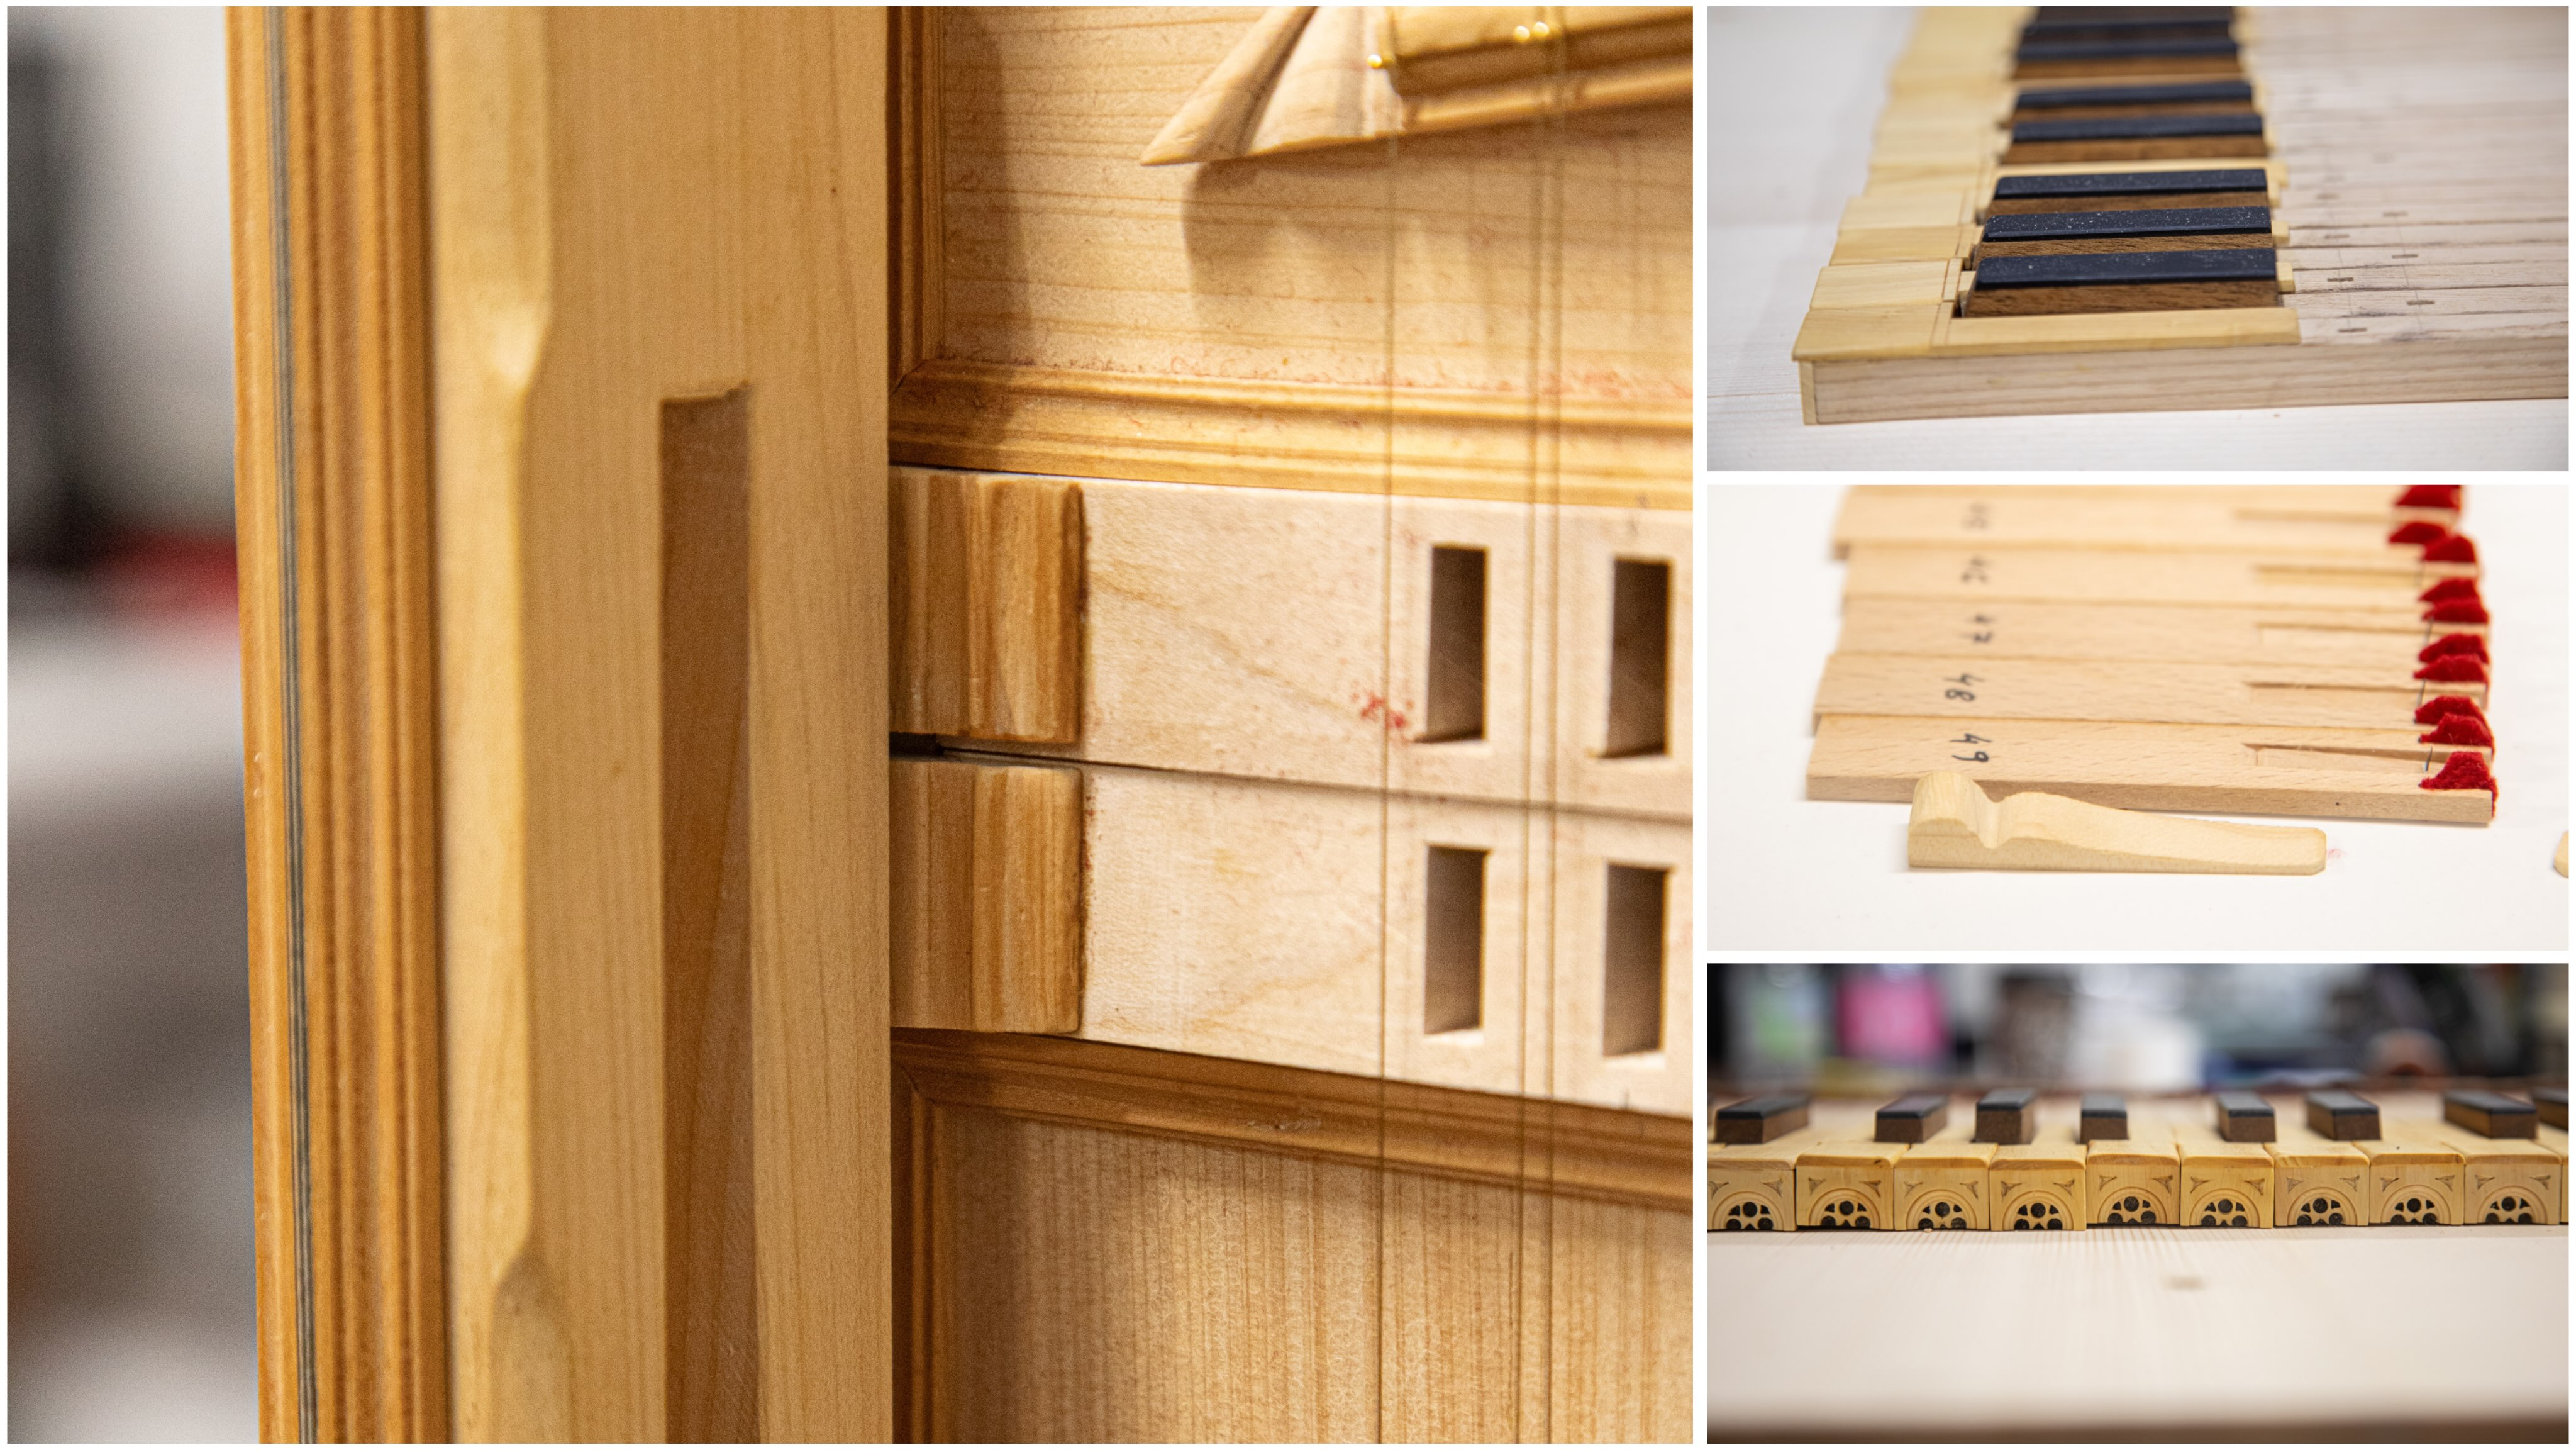
\includegraphics[width=0.8\linewidth]{img/details.jpg}
%     \caption{Details of the replica, including the key slots and sides, keys, and jacks with seagull plectra.}
%     \label{fig:details}
% \end{figure}

% \subsection{Haptic Keyboards}\label{musical-haptics}

\subsection{Terminology}

There is some confused usage of  terminology around haptic interfaces as it used
in the DMI communities such as NIME. The terminology around DMIs takes its cues
from the field of Human-Computer Interfaces (HCI) with terms for physical
sensory feedback such as haptic, tactual, tactile, vibrotactile, kinaesthetic,
proprioception, force feedback all in use, but sadly not commonly with strict
definition. This section aims will define terms relating to haptic as they
relate musical instrument interfaces in order to bring clarity to the remainder
of thesis. 

The archive of DMIs available from the NIME conference will be the primary
source of definition and for examples of usage, which is facilitated by its open
access under the Creative Commons Attribution 4.0 International License (CC BY
4.0).\footnote{\url{https://creativecommons.org/licenses/by/4.0/}}

For this thesis, `Feedback' refers to physical sensory feedback, the sense of
forces, movement, position, and pressure as sensed by the human body. 


\paragraph{Haptic Feedback:} Physical feedback that engages the sense of touch, including
tactile and kinaesthetic sensations. `Haptic' can also be substituted for tactual
when feedback is cutaneous (i.e. sensed by the skin \cite{bongers_tactual_1998, srinivasan_tactual_1996}). 
Haptic is derived from the Greek word `haptikos', meaning ``a sense of touch'' \cite{culmer_haptics_2020}. 
Oxford English dictionary defines haptics as: ``Relating to the sense of touch, in particular
relating to the perception and manipulation of objects using the senses of touch
and proprioception.''
How the term is used with respect to DMI is perhaps more pertinent.
For \textcite{omodhrain_playing_2000}, ``The term haptic refers to combined feedback from tactile sensors in the skin and kinesthetic sensors in muscles and joints.''  
\textcite{rovan_typology_2000} refers to haptics as ``Sensory and motor modalities under one unified umbrella''. Finally, haptic is defined by \textcite{cook_remutualizing_2004}` as the ``combined senses of touch, including skin vibration and pressure, and the muscle senses of motion,
position, and force)''.
From this we can understand that vibration or texture felt directly by the skin, as well as forces felt by the muscles, can all be described as haptic feedback. Given the types of physical interaction that occur in the domain of musical instruments, we will see that some of this terminology can become muddled.

\paragraph{Mechanical Feedback:} Haptic feedback using physical movement or
structures that apply forces or constraints. \textcite{rovan_typology_2000}
appears to use haptic and mechanical feedback interchangeably.
\textcite{hayes_vibrotactile_2011} refers to a ``actuator or mechanical
device''. Mechanical feedback is a less helpful distinction as it relates to
DMIs since generally all haptic feedback is mechanical feedback. This subset is
in contrast to thermal \cite{miyashita_thermoscore_2004}, ultrasonic \cite{hwang_airpiano_2017} or electrical \cite{altinsoy_electrotactile_2011} feedback where the haptic
feedback is achieved through heat, sound waves and electrical current respectively

\paragraph{Tactile feedback:} Haptic feedback as perceived through the touch and
contact to the body—including sensations like pressure, texture, or
vibration—distinct from deeper force sensations. \textcite{rovan_typology_2000}
defines tactile as ``discriminative touch as in the perception of surfaces.''
Confusingly, tactile is also used alongside `tactual' and haptics. Tactual
refers to cutaneous sensations (as felt by the skin) but also encapsulates
kinaesthetic feedback \cite{bongers_tactual_1998}. Haptic also refers to tactile
and kinaesthetic feedback, just not necessarily cutaneous in nature; however,
for DMIs the majority of cases that discuss tactile feedback are also speaking
of cutaneous feedback. This is as opposed to say, `dental feedback' which would
perhaps to relevant to the players of single reed instruments or the jaw harp
where the teeth are in contact with the instrument. It is perhaps for this
reasons that `tactual' is uncommonly used with repesct to DMIs. In fact, the
term appears only in 10 papers, mostly in citation to
\cites[x1][]{sherrick_scale_1985}[x4][]{bongers_tactual_1998}[x2][]{tan_multifinger_1996}.\footnote{Although,
only \textcite{bongers_tactual_1998} defines the term.} In the NIME archive,
`tactual' is used only four times in the paper body, three times alongside
`haptic' but without differentiation
\cite{gunther_multi_2002,pardue_hand_2013,spapetti_multi_2015} and once without
reference to haptic \cite{ferris_musical_2002} as part of ``sensory modalities
--tactual, kinaesthetic, sonic, auditory.'' though the usage is tautological as
kinaesthetic is encompassed by `tactual'. This is in contrast to `haptic', which
appears in around 300 papers. As such, haptic and tactual can be considered
relatively interchangeable as it relates to DMIs.

\paragraph{Vibrotactile Feedback:} A subset of tactile feedback achieved through
vibration. More precisely, ``vibrating at a given frequency, in contact with the
skin at one or several locations \cite{rovan_typology_2000}'' and ``using
mechanical vibration of the skin, typically at frequencies of 10-500 Hz''
\cite{kaczmarek_electrotactile_1991}

\paragraph{Kinaesthetic Feedback:} Haptic feedback that relates to the awareness
of parts, specifically their position and movement ``Kinaesthetic perception is
the awareness of the body state, including position, velocity and forces
supplied by the muscles.'' \cite{palacio_eight_2008}  `` position and motor
control of muscles and joints,'' \cite{hayes_vibrotactile_2011} ``meaning the
movement principles of the body'' \cite{bokowiec_ritual_2011}. 
Kinaesthesia, ``the sense of movement'' and the  set of cues supplied by the proprioceptors of the jnoi muscles and locomotor commands'' and proprioception as a subset of kinesthesia \cite[][p. 26 - 32]{berthoz_brain_2000}
Kinaesthetic sensation and feedback are also discussed loosely in the NIME archive with the
term being used in approximately 30 paper, but few strict definitions. For the
NIME community, kinaesthetics are often discussed alongside somatic practice and
proprioception relatively interchangeably.  
In sum, Kinaesthesia is quite an abstract concept and one that is probably
understood more by intuition than a fundamental grasp of the concept. Thus, for
its use as part of haptics in part this project it can best be summarised as how
the interface influences the movement and and encourages specific movement of
parts of the body during use. 

\paragraph{Force Feedback:} is haptic feedback derived from physical impedance \cite{giordano_force_2012} or force perceived by muscles and joints, allowing users to feel weight, resistance, or motion. Thus, force feedback can be thought of as a subset of kinaesthetic feedback \cite{kirkegaard_torquetuner_2020}.  Examples of force feedback in DMIs would be projects such as the FireFader
\cite{berdahl_firefader_2013} and TorqueTuner
\cite{kirkegaard_torquetuner_2020}. \newline
% \item Electrotactile: ``stimulation evokes tactile (touch) sensations within
% the skin at the location of the electrode by passing a local electric current
% through the skin.'' doi: 10.1109/10.68204
    
\begin{figure}
    \centering
    \begin{verbatim}
        Haptic Feedback
        ├── Mechanical        
        │   ├── Tactile      
        │   │   └── Vibrotactile
        │   └── Kinaesthetic
        │       └── Force
        ├── Thermal
        │   ├── ...
        │   ...
        ├── Electrical
        │   ├── Electrotactile
        │   ...
        ├── Ultrasonic
        │   ├── ...
        │   ...
        ...
    \end{verbatim}
        
    \caption{An incomplete, informal taxonomy of haptic feedback.}
    \label{fig:taxonomy}
\end{figure}

On top of these subsets of haptic feedback, \textcite{cook_remutualizing_2004} makes a further distinction between
``passive'' haptics and an inferred category of ``active'' haptics.
Passive haptic feedback refers to a haptics achieved by purely mechanical
means without the aid of any computation and the use of actuators or motors.
Cook puts forth weighted piano keys as an example of passive haptics. The usage
of the haptic feedback of the harpsichord jacks would also put the interface
here in `passive' category. Using the taxonomy of Figure~\ref{fig:taxonomy}, and
Cook's `passive' distinction, the interface described herein could therefore be
categorised as passive haptic, force-feedback, tactile interface. For brevity,
simply `haptic' will be used.

Since all musical instruments and interface involve physical interaction, with
the exception of perhaps the theremin, one could argue that in fact all musical
instruments are passively haptic. Keyboards, weighted or not, still require some force and
have a limited amount of travel meaning resistance will be felt. The physicality of the interface by definition means that it can be perceived through tactile or kinaesthetic senses. One could argue even
the theremin is a haptic device. Tactile feedback is famously absent in the theremin, however the instrument necessitates that the body move in a certain way, which could be argued to be a form of kinaesthetic feedback. This thesis will not discuss the ontological implications of the term haptic feedback rather the term is used herein to describe design intent.




\subsection{Haptics and Performer Perception}\label{musical-haptics} 

Research has demonstrated that the presence of kinaesthetic and tactile feedback have influence, combined or in isolation, on not just perceptions of the instrument but also influence of the sound. Further more, haptic feedback is not just influential on experience but a desired quality of an interface \cite{magnusson_survey_2007}. The quality of an instruments sound is entwined with its haptic dynamics resulting in performers ability for ``audio-kinesthetic discrepancy'' \cite{galembo_quality_2003} when evaluating an instrument.  This appear to extend to learned experience as the percussive finger-key \cite{goebl_perception_2014} and piano action noises \cite{baron_physical_1958} inform performer perceptions of dynamics and timbre \cite{fontana_perception_2018}. Haptics do not just play a comoonent with perception of instrumnent and sound quality, but are also a vital component with the skill acquisition process \cite{omodhrain_once_2018}. The coupling between  the mechanics of the instrument and the body of the performer are integral part to building a model of the instrument's behaviour during skill acquisition. Removal of this component will therefore only provide a hindrance to the learning process. \textcite{omodhrain_once_2018} suggests the anti-thesis of the dynamic system of a haptic is the touch screen, which allows control but with absence of any physical ``anchor.'' This conclusion is supported in \textcite{young_musical_2018}, where force feedback or force and tactile feedback combined are shown to have a greater influence on the perceived ``learnability'' of an interface. By extension, this becomes relevant in the museum context where a haptic interface could be more effective in encouraging curiosity in the skill of historical instrument performance. Such an interface would provide a  means to ``engage in a process of discovery'' \cite{omodhrain_once_2018} that would otherwise be absence in a purely sonic presentation.

\section{Harpsichord Mechanics}

\begin{figure}
    \centering
    \frame{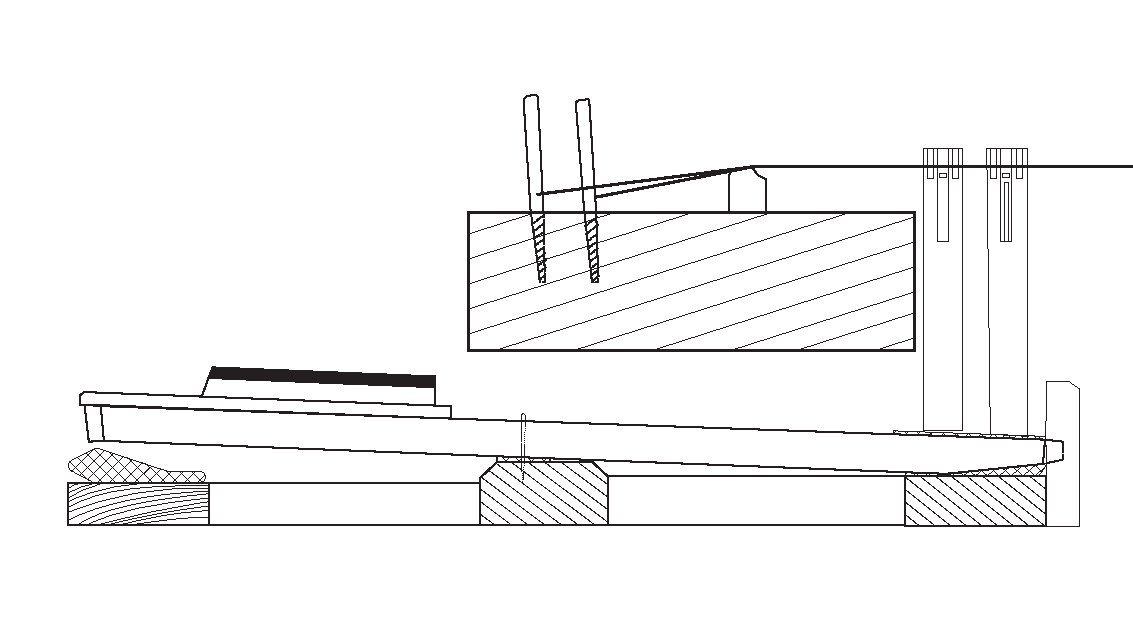
\includegraphics[width=1\linewidth]{img/drawing-3-key-mechanism.pdf}}
    \caption{Single manual, two-register action as used on the 1547 Alessandro Trasuntino and model interfaces.}
    \label{fig:mechanism}
\end{figure}

Harpsichord existed in its earliest form in the latter half of the fourteenth century and with its mechanism partly stemming from, what was referred to as the time, as an ``eschaquier'' \cite{koster_keyboard_1994} (or ``eschequier'' \cite{dewhirst_stringed_2016}) as well as the plucking action stemming from the psaltery \cite{campbell_musician_1987}.

The harpsichord mechanism consists of a second class lever that forces a plectrum upwards to pluck a string. Plectra were typically made of quill but also leather.

The plectra are attached to `jacks', two-part wooden blocks that are displaced directly by the key lever.
The two parts of the jack are the `body' and the `tongue'. The plectrum is wedged into a slot on the tongue and the tongue is attached to the body with a pin. The tongue is tapered along part of its length and the recess on the body for the tongue is similarly tapered, which allows the jack to rest in an upright position when it pushes against some kind of spring. The material used for the spring is typically strips of brass though sometimes quill and boar hair are also used \cite{tagliavini_clavicembali_1987}.

As the jack is displaced upwards the quill acts against the string. This force is translated as lateral movement towards the body of the jack, but the tapered recess ensures the tongue does not move. After the

There is a relatively fixed force to overcome the resistance of the quill against the string. As such, the volume of the harpsichord string pluck is equally fixed and it might be said these fixed dynamics are one of the defining features of the instrument.

\begin{figure}
    \centering
    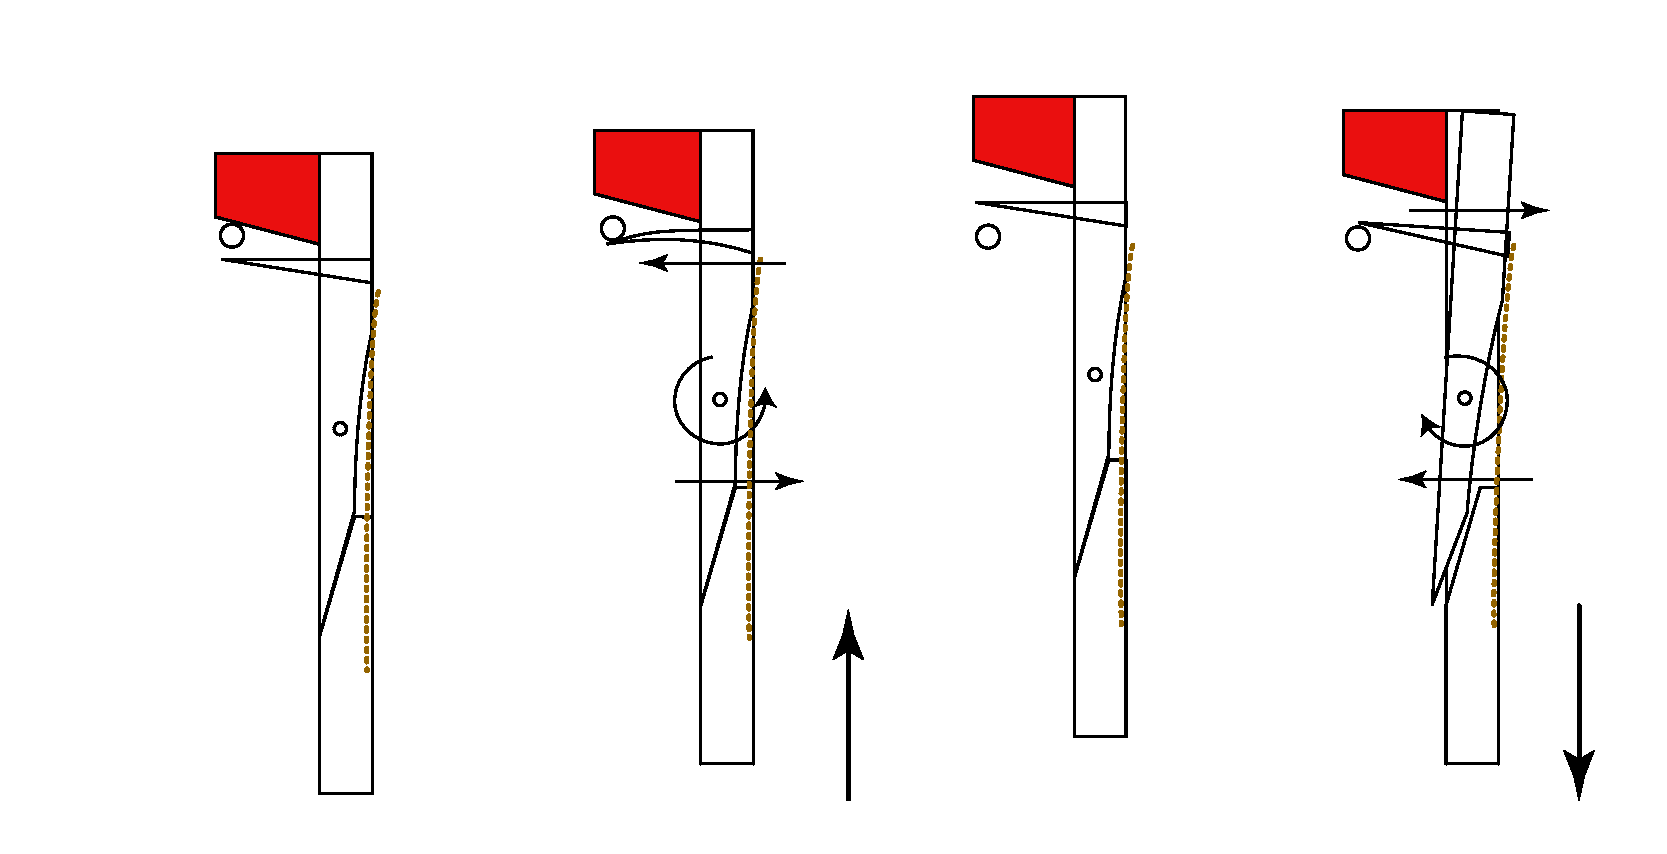
\includegraphics[width=0.5\linewidth]{img/drawing-jack_forces.pdf}\\
    
    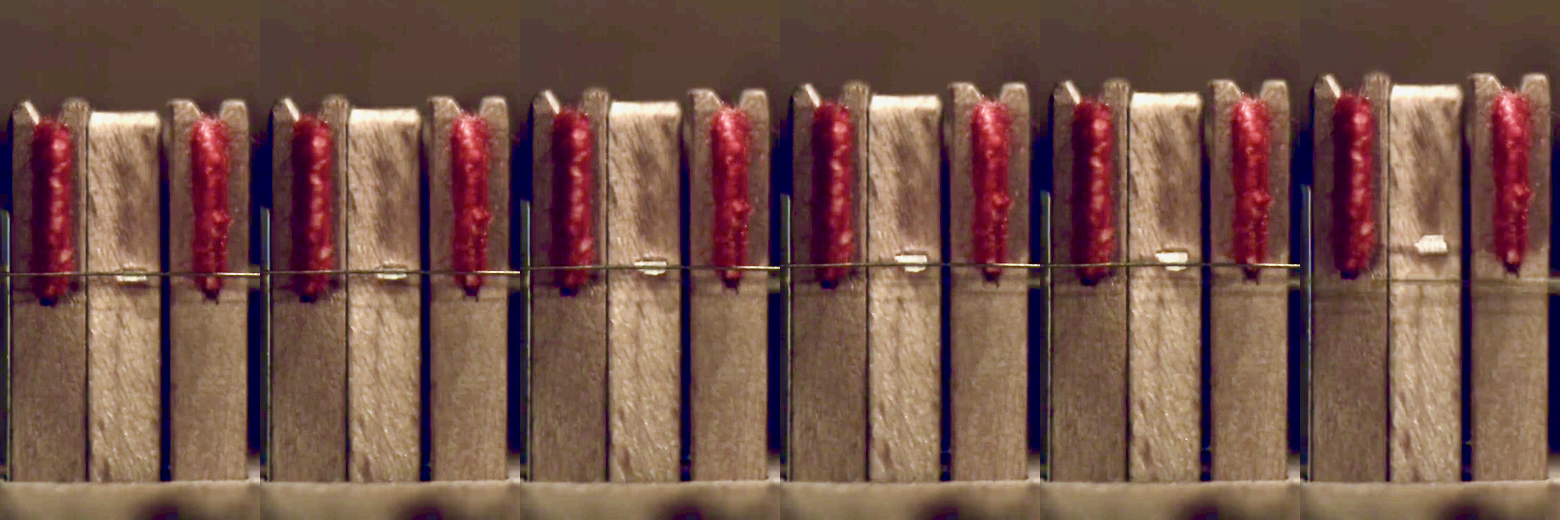
\includegraphics[width=0.5\linewidth]{img/film-strip.jpeg}
    \caption{Forces at play on the jack during the plucking and release phases (Adapted from  \textcite[Figure 1.7][]{perng_physical_2012}) against a 1000 frames per second photo series illustrating jack displacement.}
    \label{fig:mechanism}
\end{figure}

By the 16th century it was typical for Italian harpsichords to have more than one string per key and each string with its own jack. In the case of multiple strings (or registers), the jacks are arranged into rows. The jacks are staggered in height in order that, during the keys' travel,  each register is plucked in turn rather than occurring simultaneously  \cite{veroli_optimising_2012}. The central problem to be solved is the detection of the moment a string is plucked by a plectrum (Figure~\ref{fig:pluck}). Since each jack is constructed by hand, the resulting subtle variations in pluck points across the entire keyboard mean that individual jack displacement must be obtained, rather than simply the displacement of the key.

% \begin{figure}
%   \centering
%   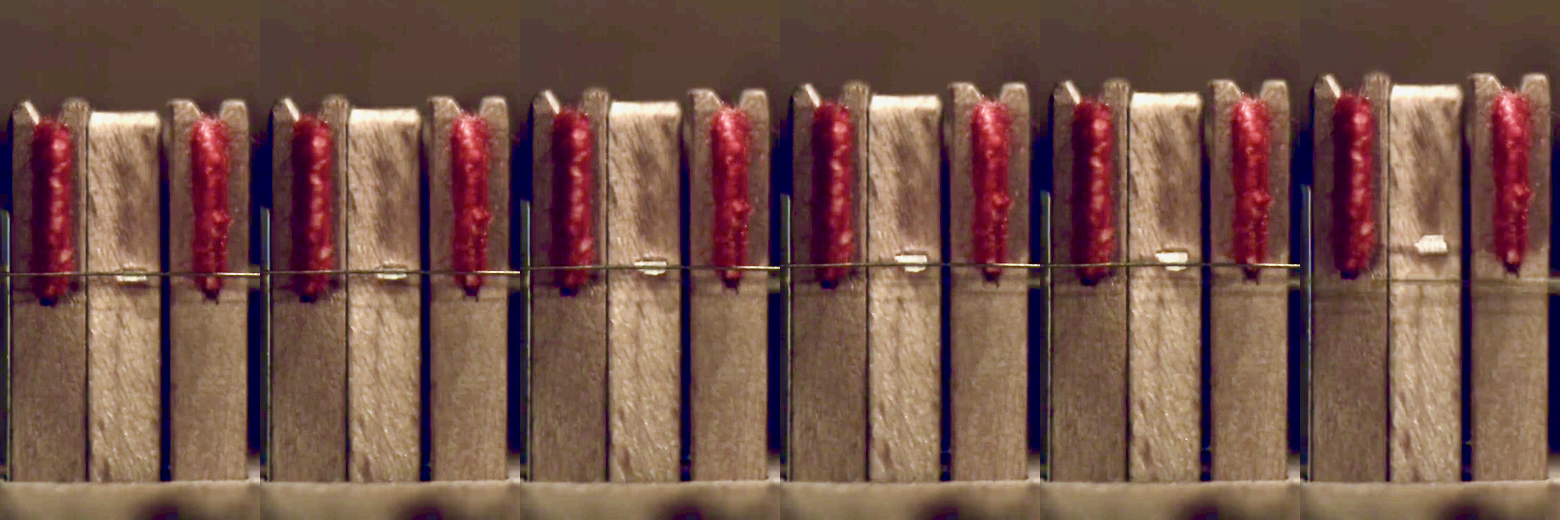
\includegraphics[width=1\linewidth]{img/film-strip.jpeg}
%   \caption{Photo series from a recording at 1000 frames per second illustrating jack displacement with the final frames are sequential and showing the pluck of the string.}
%   \label{fig:pluck}
% \end{figure}

\textcite{oboe_mikey_2006} defines force profile of the harpsichord for forward travel (key depression) as:
\begin{equation}
f(t) = B\dot{\theta}(t) + X(\theta(t))
\end{equation}

\begin{itemize}
    \item \(f\) a function of force applied to key over time \(t\)
    \item \(\theta\) a function of angular displacement, in time \(t\)
    \item \(B\) a viscosity friction constant, the \(\dot{\theta}\) velocity with \(B \dot{\theta}\) comprising the viscous damping term.
    \item \(X\) a function of \(\theta\) representing ``extra terms''
\end{itemize}

\section{Design Constraints}\label{sec:design-constraints}

Two sets of design constraints were drawn up, one for the final mechanical interface and another for the
electronic sensor system. These constraints provided pillars on which to guide the design process and a set of criteria by which the mechanics and electronics could be evaluated.

\subsection{Mechanical Interface}

The design of the augmented replica keyboard for the Museo San Colombano was guided by these criteria:

\begin{itemize}
    \item \emph{Faithfulness}. The keyboard mechanism had to ensure fidelity to
    its authentic operation. The electronics system would not seek to `fix' or
    `improve' the limitations of the original design.     
    \item \emph{Robustness and reliability}. The system needed to accommodate
    frequent use by museum visitors and allow for straightforward maintenance by
    staff without requiring specialised technical expertise.
    \item \emph{No visible electronic components}. To preserve the visual
    integrity of the exhibit, all electronic components had to remain concealed
    except for a pair of headphones and a small display for audio parameter
    adjustments.
    \item \emph{Reduced use of space}. As museums often face space limitations,
    the instrument needed be compact enough not to compromise space for
    exhibition of the permanent display. 
\end{itemize}

These constraints cascaded to the constraints of the  electronics system, requiring that it be non-invasive in design and respectful of the instruments' historical aesthetics. The requirement for
faithfulness to the original mechanism immediately ruled out a mechanical design
reliant on electromechanical actuators, as in previous works on piano haptics
\cite{timmermans_multibody-based_2020,gillespie_haptic_1996}. While actuators
can generate considerable force, achieving a jack's free motion and resistance
is difficult without extensive mechanical intervention such as that carried out
by Gillespie \cite{gillespie_haptic_1996}.

% The final design, shown in Figures \ref{fig:teaser} and \ref{fig:details}, is a
% 49-key, two-register harpsichord keyboard replica. 

\begin{figure}  
  \centering
  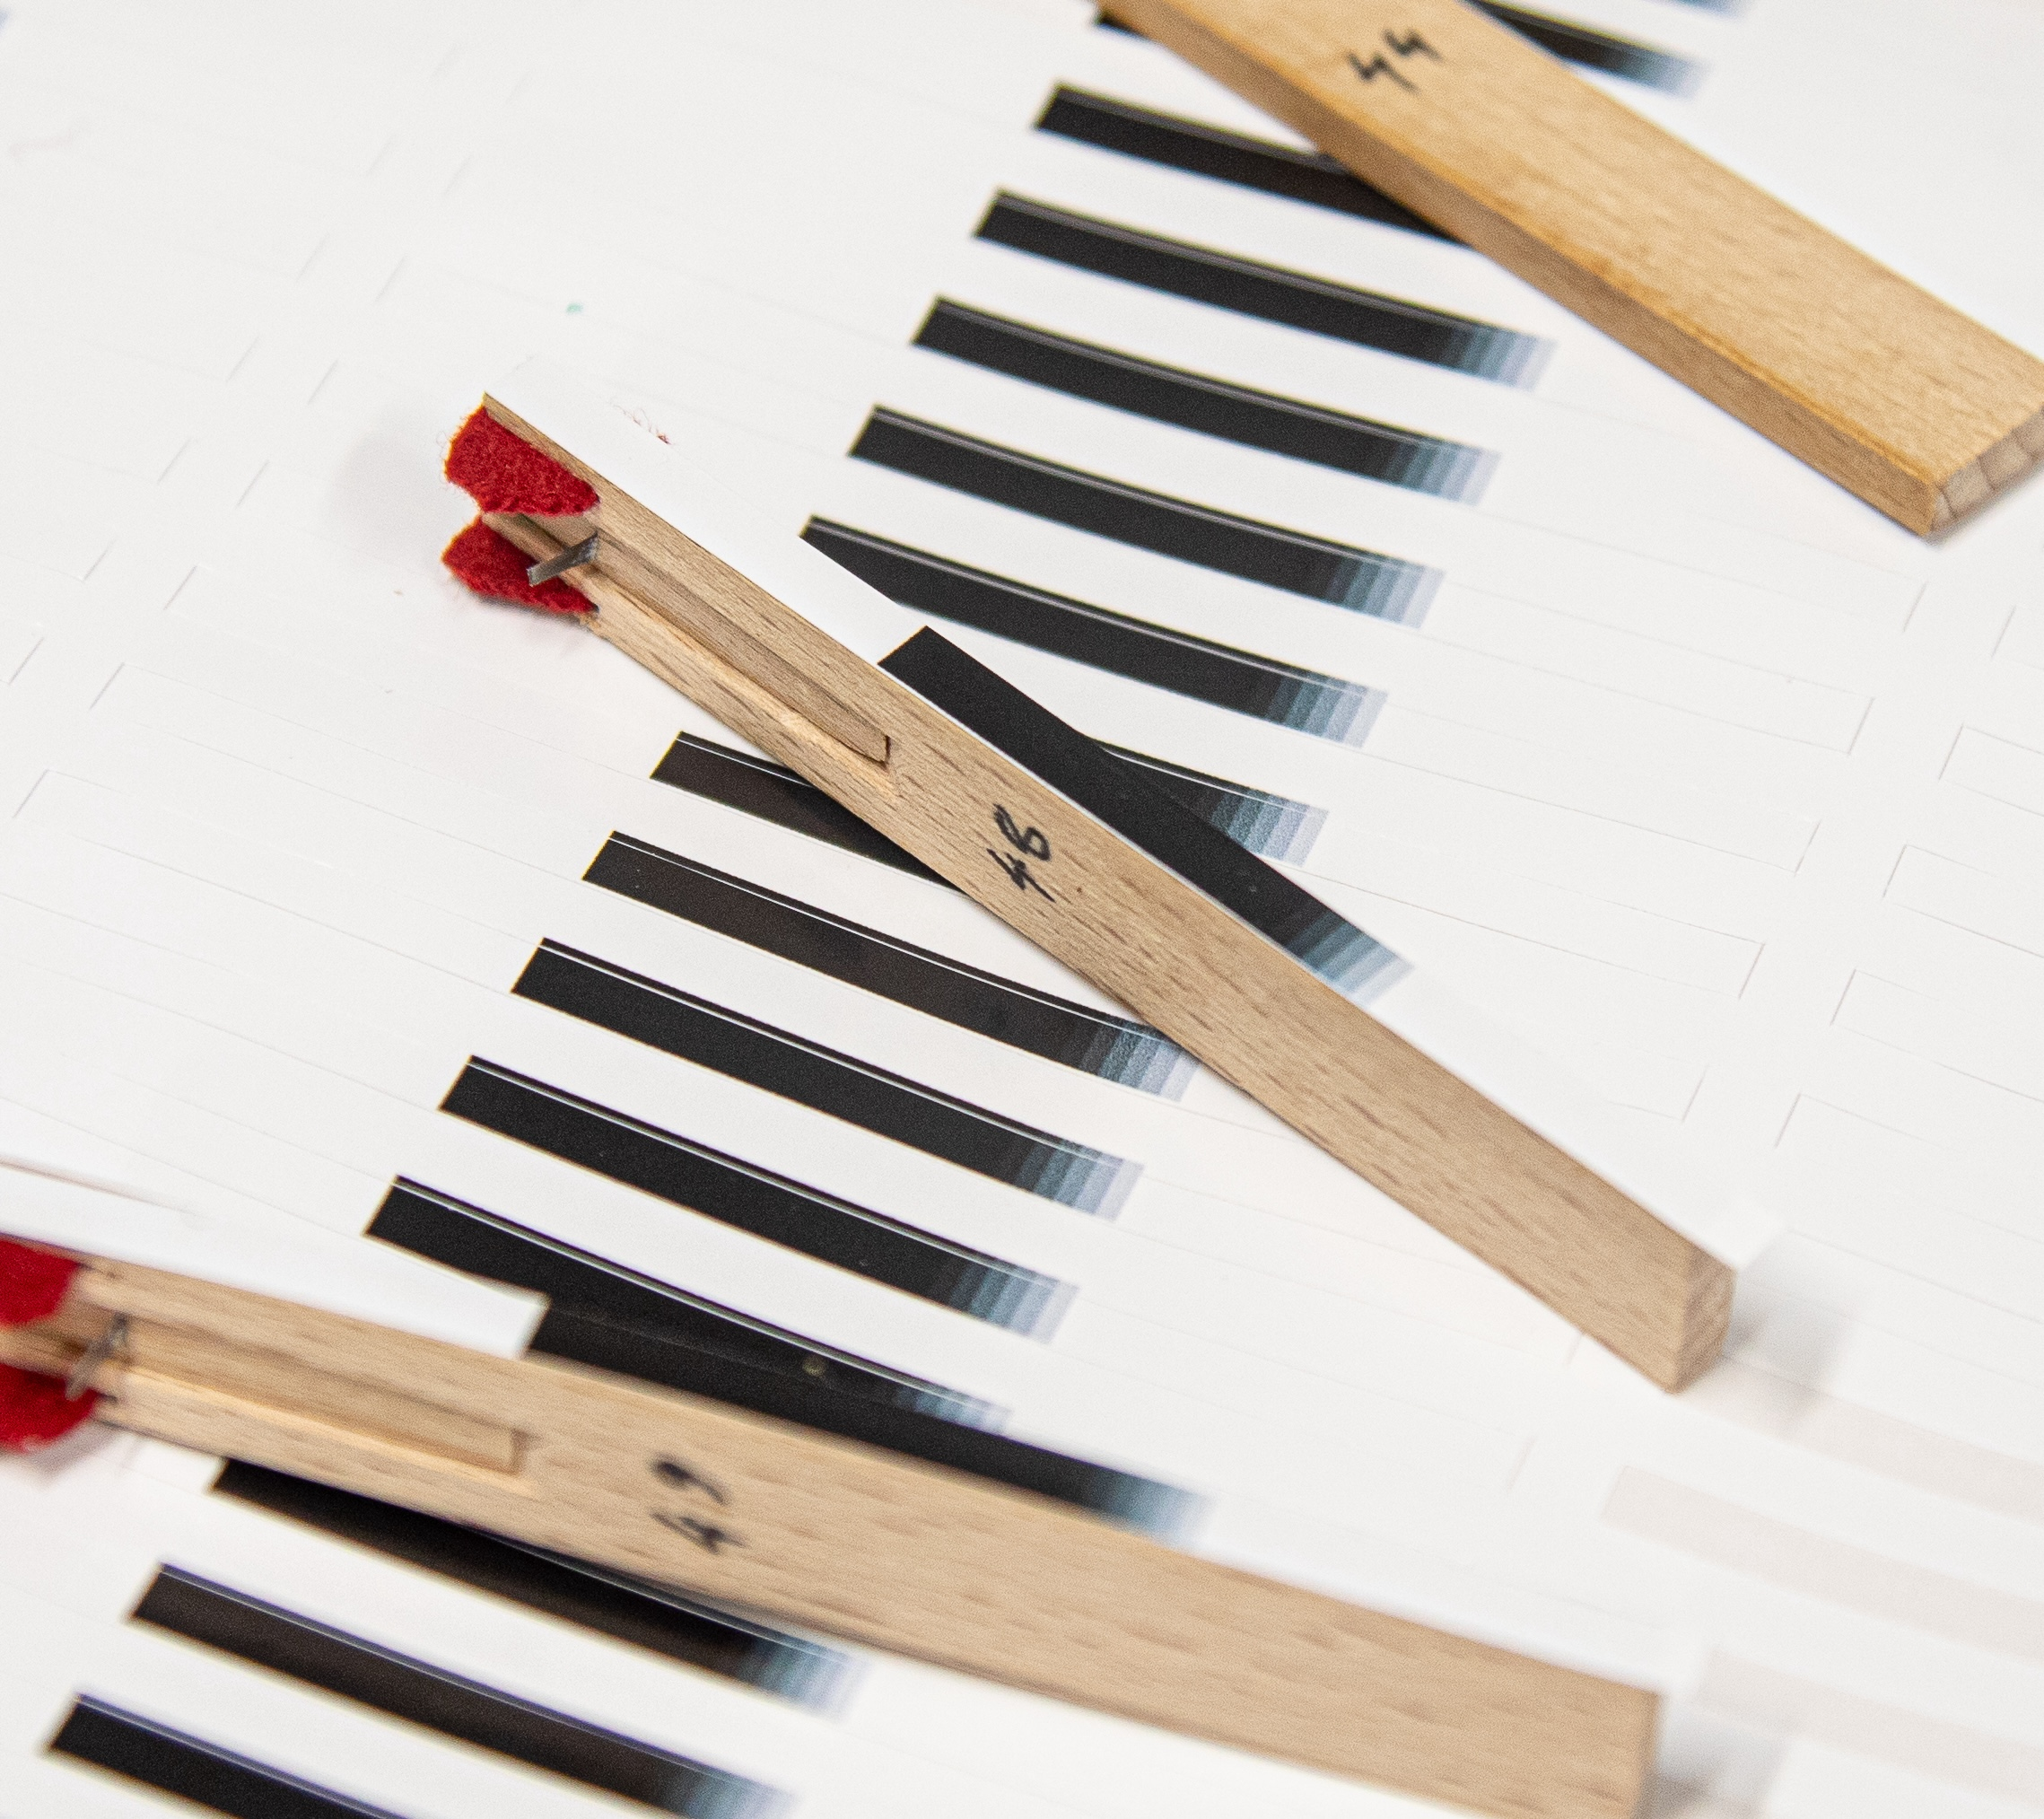
\includegraphics[width=0.66\linewidth,trim={0 0 0 0.5cm},clip]{img/tagging-jacks-3.jpg} 
  \caption{Gradient stickers applied to the side of the jack body. The coarse gradient scale was selected to maximise signal excursion while preserving signal readout stability.}

  \label{fig:jack-tags}
\end{figure}

Optical sensors are positioned in front of each jack and their output voltage
depends on the amount of light reflected from a sensor surface. In this case,
the sensor surface is a grey-scale gradient printed on a vinyl sticker (Figure
\ref{fig:jack-tags}) and applied to the side of each jack. Though the current
configuration simply sends MIDI note-on and -off messages when passing a
threshold, the displacement of all jacks is available continuously. The jacks
for a single key typically have their pluck points offset from each other, a
practice known as `staggering'. A combination of string tension, quill voicing,
and jack staggering contribute to the overall resistance of the action, with
each key differing from the low to the high octaves
\cite{veroli_optimising_2012}. The staggering of the pluck point of the jacks
between registers means that there are two distinct tactile anchors along the
key dip. The current sensor system enables the data recording of traditional use
from which it can be identified where those opportunities for new expression lie
\cite{mcpherson_space_2013}.

\begin{figure}
  \centering
  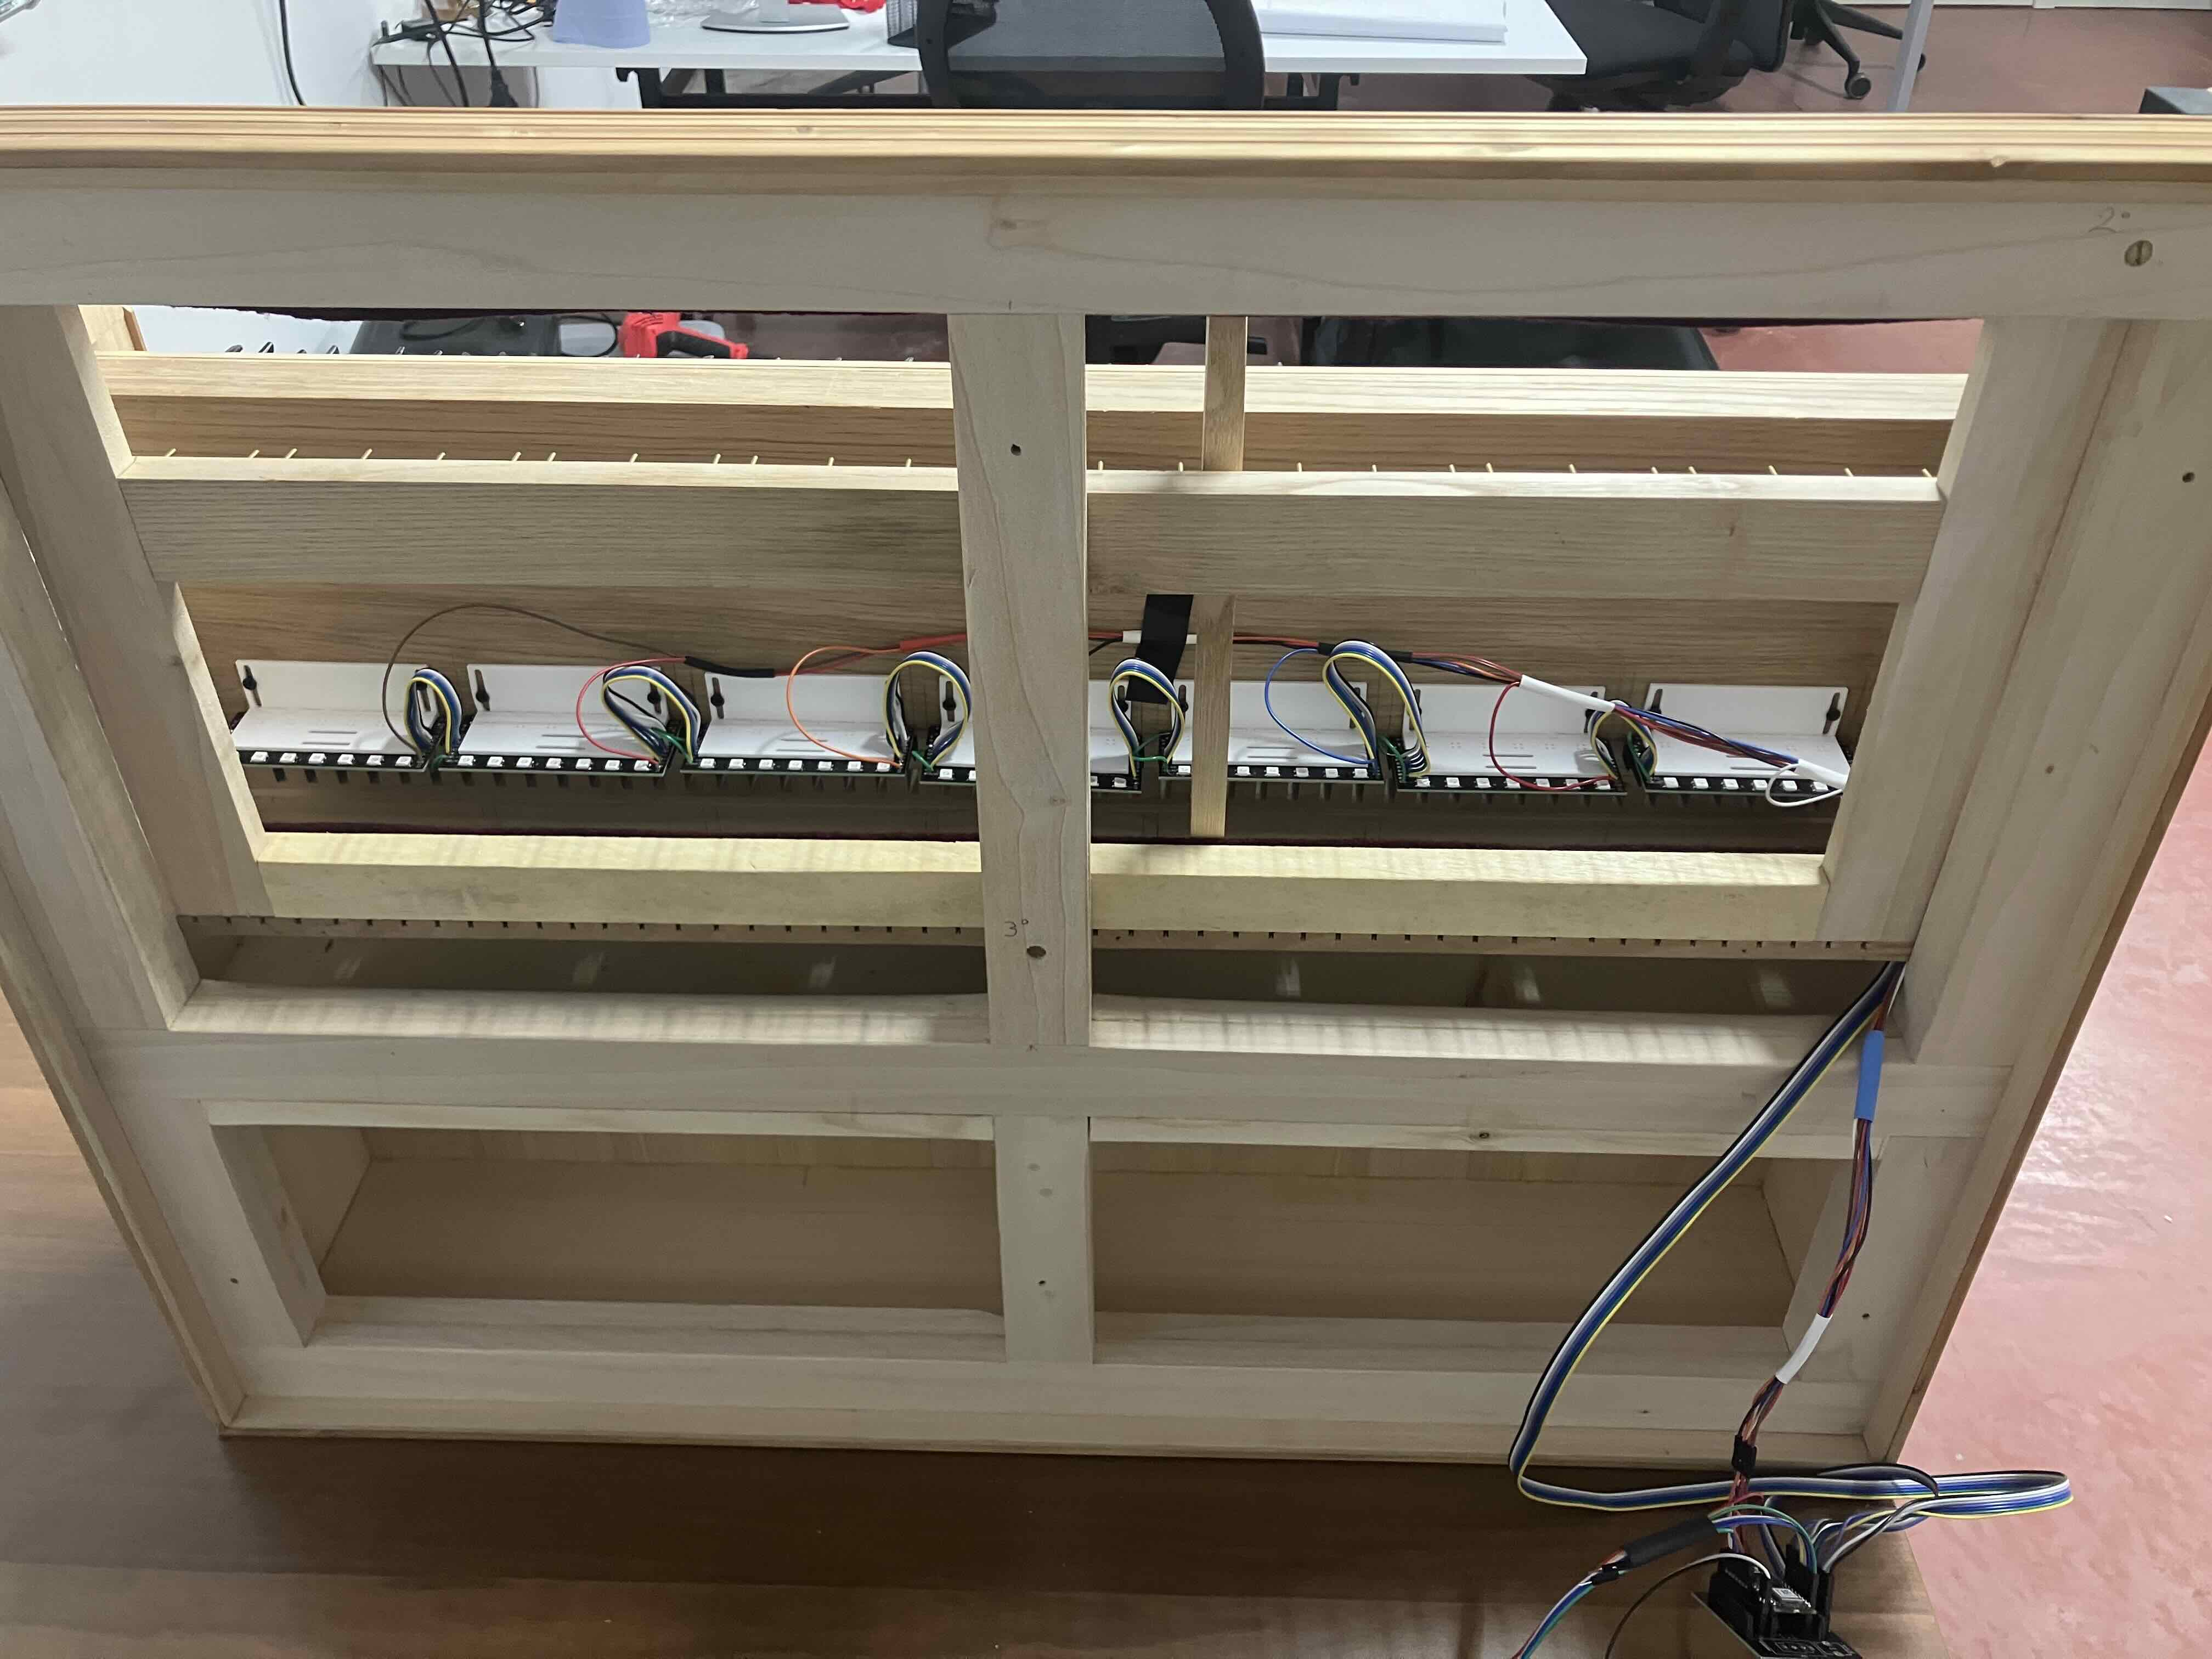
\includegraphics[width=\linewidth]{img/mark-1-bottom-sensors-no-keys.jpg} 
  \caption{Underside of the full model keyboard, showing two chambers: the front chamber (top) and the rear chamber (bottom).} 

  \label{fig:mark-1-bottom}
\end{figure}

A modular system of printed circuit boards (PCBs) was designed to manage the
sensors and process their output. The system uses 49 optical sensors distributed
across seven boards containing seven sensors each. The PCBs were secured to the
underside of the wrest plank and above the keys (Figure
\ref{fig:mark-1-bottom}), allowing them to be adjusted during installation.
Ribbon cables connected the PCBs, providing flexibility during assembly while
maintaining a compact form factor. Additional modifications, including baffles
and adhesive improvements, were made to optimise the reliability of the sensor
system during calibration and use.

The project expanded upon earlier NIME research on generating MIDI messages from
piano keystrokes \cite{mcpherson_portable_2013}, adapting it to address the
specific characteristics of harpsichords. Whereas the previous design emphasised
continuous gesture tracking, this implementation required discrete key-triggered
data to align with the needs of MIDI-triggered audio playback. 

\subsection{Electronics}

The following criteria were established to guide sensor selection and
integration to make the system suitable for a museum context:

\begin{itemize}
    \item \emph{Non-invasiveness:} No remarkable modifications were allowed on
    the harpsichord mechanics, particularly on all the visible parts.
    \item \emph{Low Latency:} The sampling period for reading and processing
    data from all sensors should remain under 10 ms to allow for latency
    introduced in other parts of the synthesis process. Empirical criteria found
    in previous studies \cite{jack_effect_2016} was used as a guide.
    \item \emph{Reliability:} Sensor data should be dependable and consistent,
    with interference from anything external to the jack movement being absent
    or negligible.
    \item \emph{Scalability:} The design needed to scale in both cost and time
    in order to be adaptable from a 3-key prototype (Figure \ref{fig:3key}) up
    to the 49 keys of the final design.    
\end{itemize}

The hardware was designed to make assembly possible in standard university maker
spaces and using economic soldering equipment. This was in part a decision made by necessity to allow for development to continue taking place regardless of location. Keeping with the open source spirit of the project, it also eschewed design and component choices that would be prohibitively expensive. Though the designs, CAD files, source code is all free, the components themselves still need to be paid for. For every expense all complexity added to the fabrication process a greater number of people effectively become `locked out'.

\begin{figure}
    \centering
    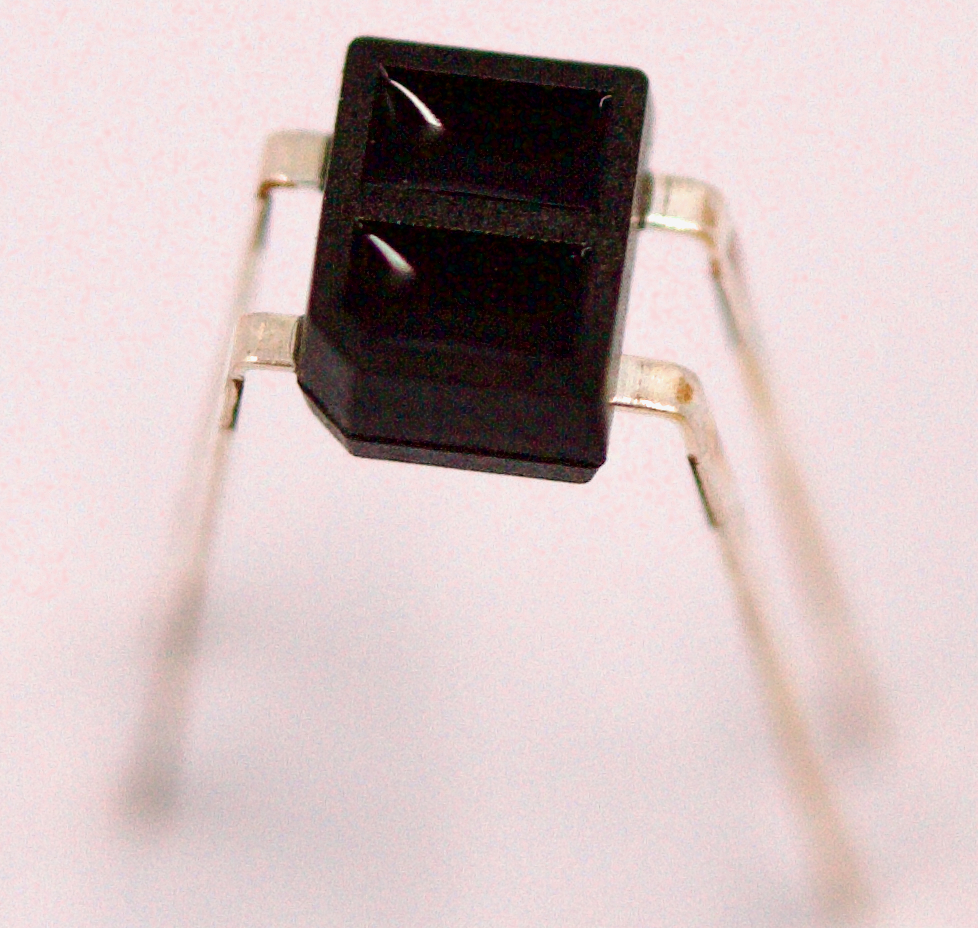
\includegraphics[width=0.5\linewidth]{img/qre-1.jpeg}
    \caption{Optical sensor in a THT form with long connectors that are trimmed after soldering.}
    \label{fig:qre-tht}
\end{figure}

Where possible, through-hole mount technology (THT) electronic components were used. THT components have contacts that extend and pass through drilled slots on a PCB and in most cases used with prototyping `breadboard'. As a result, THT parts are self-locating much easer to solder with economic soldering equipment. By contrast, there are surface mount device (SMD) components, which instead of being soldered to a through hole, are soldered directly to `pads' on a PCB. SMD component can therefore be much smaller compared to their THT equivalent, saving on space. SMD components cannot be used with a breadboard as such they are used in function with a connector board or in the final design of a PCB. Such component can be soldered by hand, but with difficulty there smaller form making it hard to locate on solder pads. Typically SMD component would be attached using by first using a solder paste stencil, placing the components which are then fixed in place by applying a hot-air solder gun. This stage can also be carried out through automated computer aided manufacture. In either case extra costs through additional labour or equipment are incurred. Finally, SMD components are not easily removed and replaced. By using THT, parts can be exchanged more easily simply mounted using headers providing greater robustness against incorrect wiring or modification of PCBs circuits after manufacture. This was especially helpful in the early prototyping stages where many mistakes would be and experimentation would be required.

\section{Prototype}

The prototyping for the sensor system was separated into multiple stages of ever increasing complexity.
The intention behind this was to solve the problem of sensing a harpsichord jack displacement in the
simplest case before moving on to more complex systems. Prototyping was to first take place on single action, then an action with multiple registers and finally expanding to an interface with multiple keys. 
The system evolved through iterative prototyping, beginning with
simple threshold-based testing and ending in a fully functional multi-sensor
interface capable of triggering MIDI events. 

The initial stage of development focused on testing whether sensor data could
reliably trigger MIDI playback. Modifying an existing harpsichord for testing
was considered but ultimately discarded due to significant internal measurement
and layout discrepancies. Instead, a custom 3-key harpsichord mechanism (Figure
\ref{fig:3key}) was used as a foundation for prototyping. This approach followed
a methodology similar to that used in the \textcite{timmermans_multibody-based_2020} Haptic Key
project, since the 3-key model enabled
iterative testing of individual components, including sensor placement, signal
processing, and mechanical tolerances, before eventually scaling the concept to a multi-octave keyobard. 

\subsection{Methodology}

The original design was to take a similar approach to the project by \textcite{timmermans_multibody-based_2020}, which itself was an extension of the methodology by \textcite{gillespie_haptic_1996} where a single model piano key action was used. More specific to the harpsichord was the experimental setup in \textcite{perng_physical_2012} which was constructed from spare parts obtained from a local luthier. The benefit of such a system would was the consideration of only a single action in isolation as well as the easy access open sided single action models permitted. 

Luckily, with the assistance on Museo San Colombano, a small model containing three harpsichord actions was procured by the NEMUS project (Figure~\ref{fig:3-key-model}). The construction of the model were after a XXXX Italian harpsichord with two registers. The cross-sectional construction permitted easy access to the key lever and jacks directly and therefore allowed simple means of mounting multiple sensors for testing. The multiple keys and registers meant that more complex iterations of the sensor system could be expanded on the same model without having to construct or procure another. The aesthetics of the model also complied with the visual requirements as set out in the design principles.
Should the prototype be used as part of a user study, this would provide some control and visual continuity between it and the final interface.

\subsection{Sensors Trials}\label{failed-sensors}

A number of sensors were trialled before the final system was decided upon, each of which was evaluated
against the design principles and constraints

An inertial measurment unit (IMU) was mounted to a single key which contained a 6
degrees of freedome acceleromoetr and gyroscope. The IMU provided a consistent set of
conditions (or signal fingerprint) from which to trigger sound, but these conditions were not easily differentiable when other
keys were pressed. Furthermore, the cost of a single IMU could be reduced when
purchased in bulk, but was far greater than other sensors that were trialled.

Two magentic-based sensors, a reed switch and a hall sensor, were trialled. Both sensors were fixed to the wrestplank and magnets embedded within the body of the jacks. 
The hall and reed sensors both provided a consistent means of
detecting a threshold. 

Reed switch consist of two flexible ferromagnetic metal contacts in a sealed glass tube with containing an inert gas or a vacuum. 
The contacts are arrange in such a way that a strong enough magnetic field will force the contacts to make or break a circuit.
A magnets can be attached to the jack so that it interacts with the reed switch at the pluck point. 
The reed can also be mounted in such a way to allow for fine adjustment. However, this places calibration in entirely the physical domain and the scalability of such a solution was not viable for the intended function. 
The hall sensors could be partially calibrated physically by adjusting their position and then further refined in software, however the process to do so for a single key was considered too time consuming.
Making the sensors adjustable was also not considered feasible given the constraints on the internal space. 
Finally embedding magnets into the jack body was also did not satisfy the criteria of being non-invasive and also posed too much risk of potential damage.

A light dependant resistor (LDR) was trialled by mounting it to the jack rail, which sits above the jacks to limit there movement after plucking. As jacks moved towards the rail, they would reduce the
light that was let through to the sensors. The LDR provided a signal from which plucks could be determined, however they were very sensitive to lighting conditions. This would mean any change in lighting would need to be accounted for, all a separate light balance system would need to be connected to compensate. The LDRs would also need to be installed outside of the internal cavity meant hiding the remainder of the electronics would be more difficult. Though the LDR was not ultimately used, it did imply that perhaps light could be used so long as it could be supplied localy and not be visible to the user.

This line of enquiry led to following from the work in \textcite{mcpherson_portable_2013, moro_platform_2020}. A system was created using the Fairchild QRE1113 \footnote{Fairchild, now ON Semiconductor, QRE1113 datasheet \url{https://www.onsemi.com/download/data-sheet/pdf/qre1113-d.pdf}}. 

\begin{figure}
  \centering
  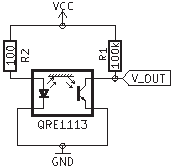
\includegraphics[width=0.5\linewidth]{img/qre1113-schematic.pdf} 
  \caption{Optical sensor in a simple voltage divider circuit.}
  \label{fig:simple-schematic}
\end{figure}


The QRE1113 is an optical sensor composed of an infrared (IR) LED and a phototransistor sensitive to IR light (Figure~\ref{fig:simple-schematic}). The optical sensor can wired in a simple voltage divider circuit such as in Figure~\ref{fig:simple-schematic}. In this configuration,  the
phototransistor of QRE1113 provides a signal on how much IR light is present, more precisely how much IR light is reflected by a surface from the LED. Since reflected
light will be proportional to the distance of a surface QRE1113 typically functions as a
close-proximity distance sensor. Distance is the way in which the instruments
in \cite{mcpherson_portable_2013, moro_platform_2020} function as well the Moog Piano Bar from
which those projects took inspiration. However, those projects focussed on the displacement of the key. For the harpsichord, the optical sensor would need to provide data on the displacement of the jacks. To take the same approach, the optical sensors would need to be mounted in the jack rail and, as was discussed with the LDR, it would be too difficult to hide the sensors from view. In order to fit the sensors internally, they would need to be directed perpendicular to the movement of the jacks.

To address this restriction on orientation, we looked toward another common application of the QRE1113, which is as the central component of line following robots \cite{ramesh_turning_2017}. 
For a line following robot,
an array of optical sensors are used in conjunction with either low or high reflectance tape. A
motorised system can then use this data to follow the line of tape, the reflectance providing a clear reference, and adjust
its position accordingly. The same principles was used, but rather than single shade, a greyscale gradient was applied to the jack body (Figure~\ref{fig:jack-tags}).

For the first iteration and as a proof of concept, the gradient was printed on an inkjet printer and attached to the jack body with double-sided
tape. For the final iteration the gradients were printed on a permanent adhesive vinyl material
\footnote{Coala, 1D 100 Gloss P, gloss, white, 300g/m2, 100 µm, 1370mm x 50.00m} using a HP Latex 115 large format printer. The print was then passed through a Summa 150 roll
cutter along with a vector file with the sticker outline. The cutter roll provided an accurate means to cut the gradients to the correct dimensions for the jack body as well as allow for surplus printing to accommodate wastage. The combined printer and cutter process greatly reduced the amount of manual labour, which meant here was compliance with the \textit{Scalability} criterion when moving from the six jacks of the prototype to the 98 jacks of the Mark 1 model.

The divider circuit resistor's, \texttt{R1} in Figure~\ref{fig:simple-schematic}, value was chosen though experimentation for best range of voltage at a distance of six millimetres from the sensor surface. A one mega-ohm potentiometer was used as a variable resistor within the voltage divider circuit. Once a desirable voltage range was found while monitoring the ADC channel, resistance across the potentiometer pins was measured to provide a guideline fixed resistor value.

The initial sensor surface design contained only the gradient and no excess material. It was
found that this approach resulted in the jacks becoming stuck in their slots as they push the edge of the surface against the walls of the jack slot. Furthermore, surface edges ending in havy ink print tended to curl, exacerbating this problem further.
The stickers were redesigned to be cover the full
length of the jack, providing a greater surface area and thus better adherence to the jack body. The longer length meant there was no printing near the edge, which solved the problem of curling edges. 

During testing it was found that their was a considerable amount cross-talk
between adjacent sensors. This meant the reading from key would be affected by
the movement of the key next to it. The cross-talk was assumed to be as a result
of light reflecting from other jacks. Given that IR is used this was difficult
to confirm by sight. A set of baffles was designed for the PCB that would wrap
round the jack and stop light from other jacks or sensors. The baffles were
printed on a BAMBU X1 3D printers using polylactic acid (PLA) plastic. 
A dark pigmented PLA was used to avoid IR light simply being diffused. After the baffles were fitted, the cross-talk was eliminated.

\subsection{Prototype PCB}

\begin{figure}
    \centering
    \includesvg[inkscapelatex=false,width=0.75\linewidth]{img/pcb-miniboard-schematic.svg} \\
    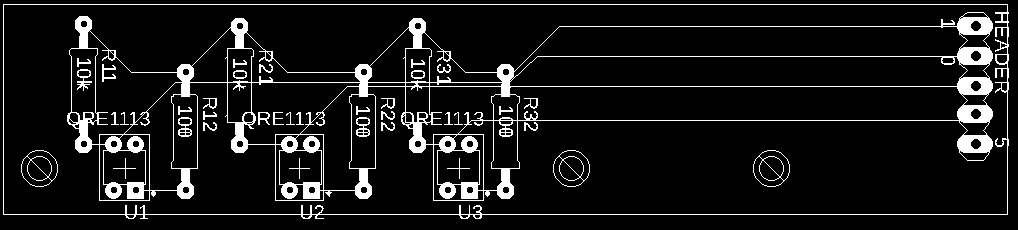
\includegraphics[width=0.75\linewidth]{img/pcb-prototype-mini-board-bw.png}
    \caption{PCB schematic of the prototype sensor board and its board silkscreen.}
    \label{fig:prototype-pcb}
\end{figure}

A prototype PCB (Figure~\ref{fig:prototype-pcb}) was drafted using the EAGLE CAD software. The prototype PCB is provides simple wiring for the optical sensors in a voltage divider configuration. The power rail for the sensors and output signals terminates in a header to allow for easy connection to a microcontroller. This PCB was create primarily as means to test the mounting of the sensors and whether variation in jack pitch spacing would be a problem. The original intention was to mount the sensors at right angle which would necessitate bending the connectors (Figure~\ref{prototype-pcb-mount}) 

\begin{figure}
    \centering
    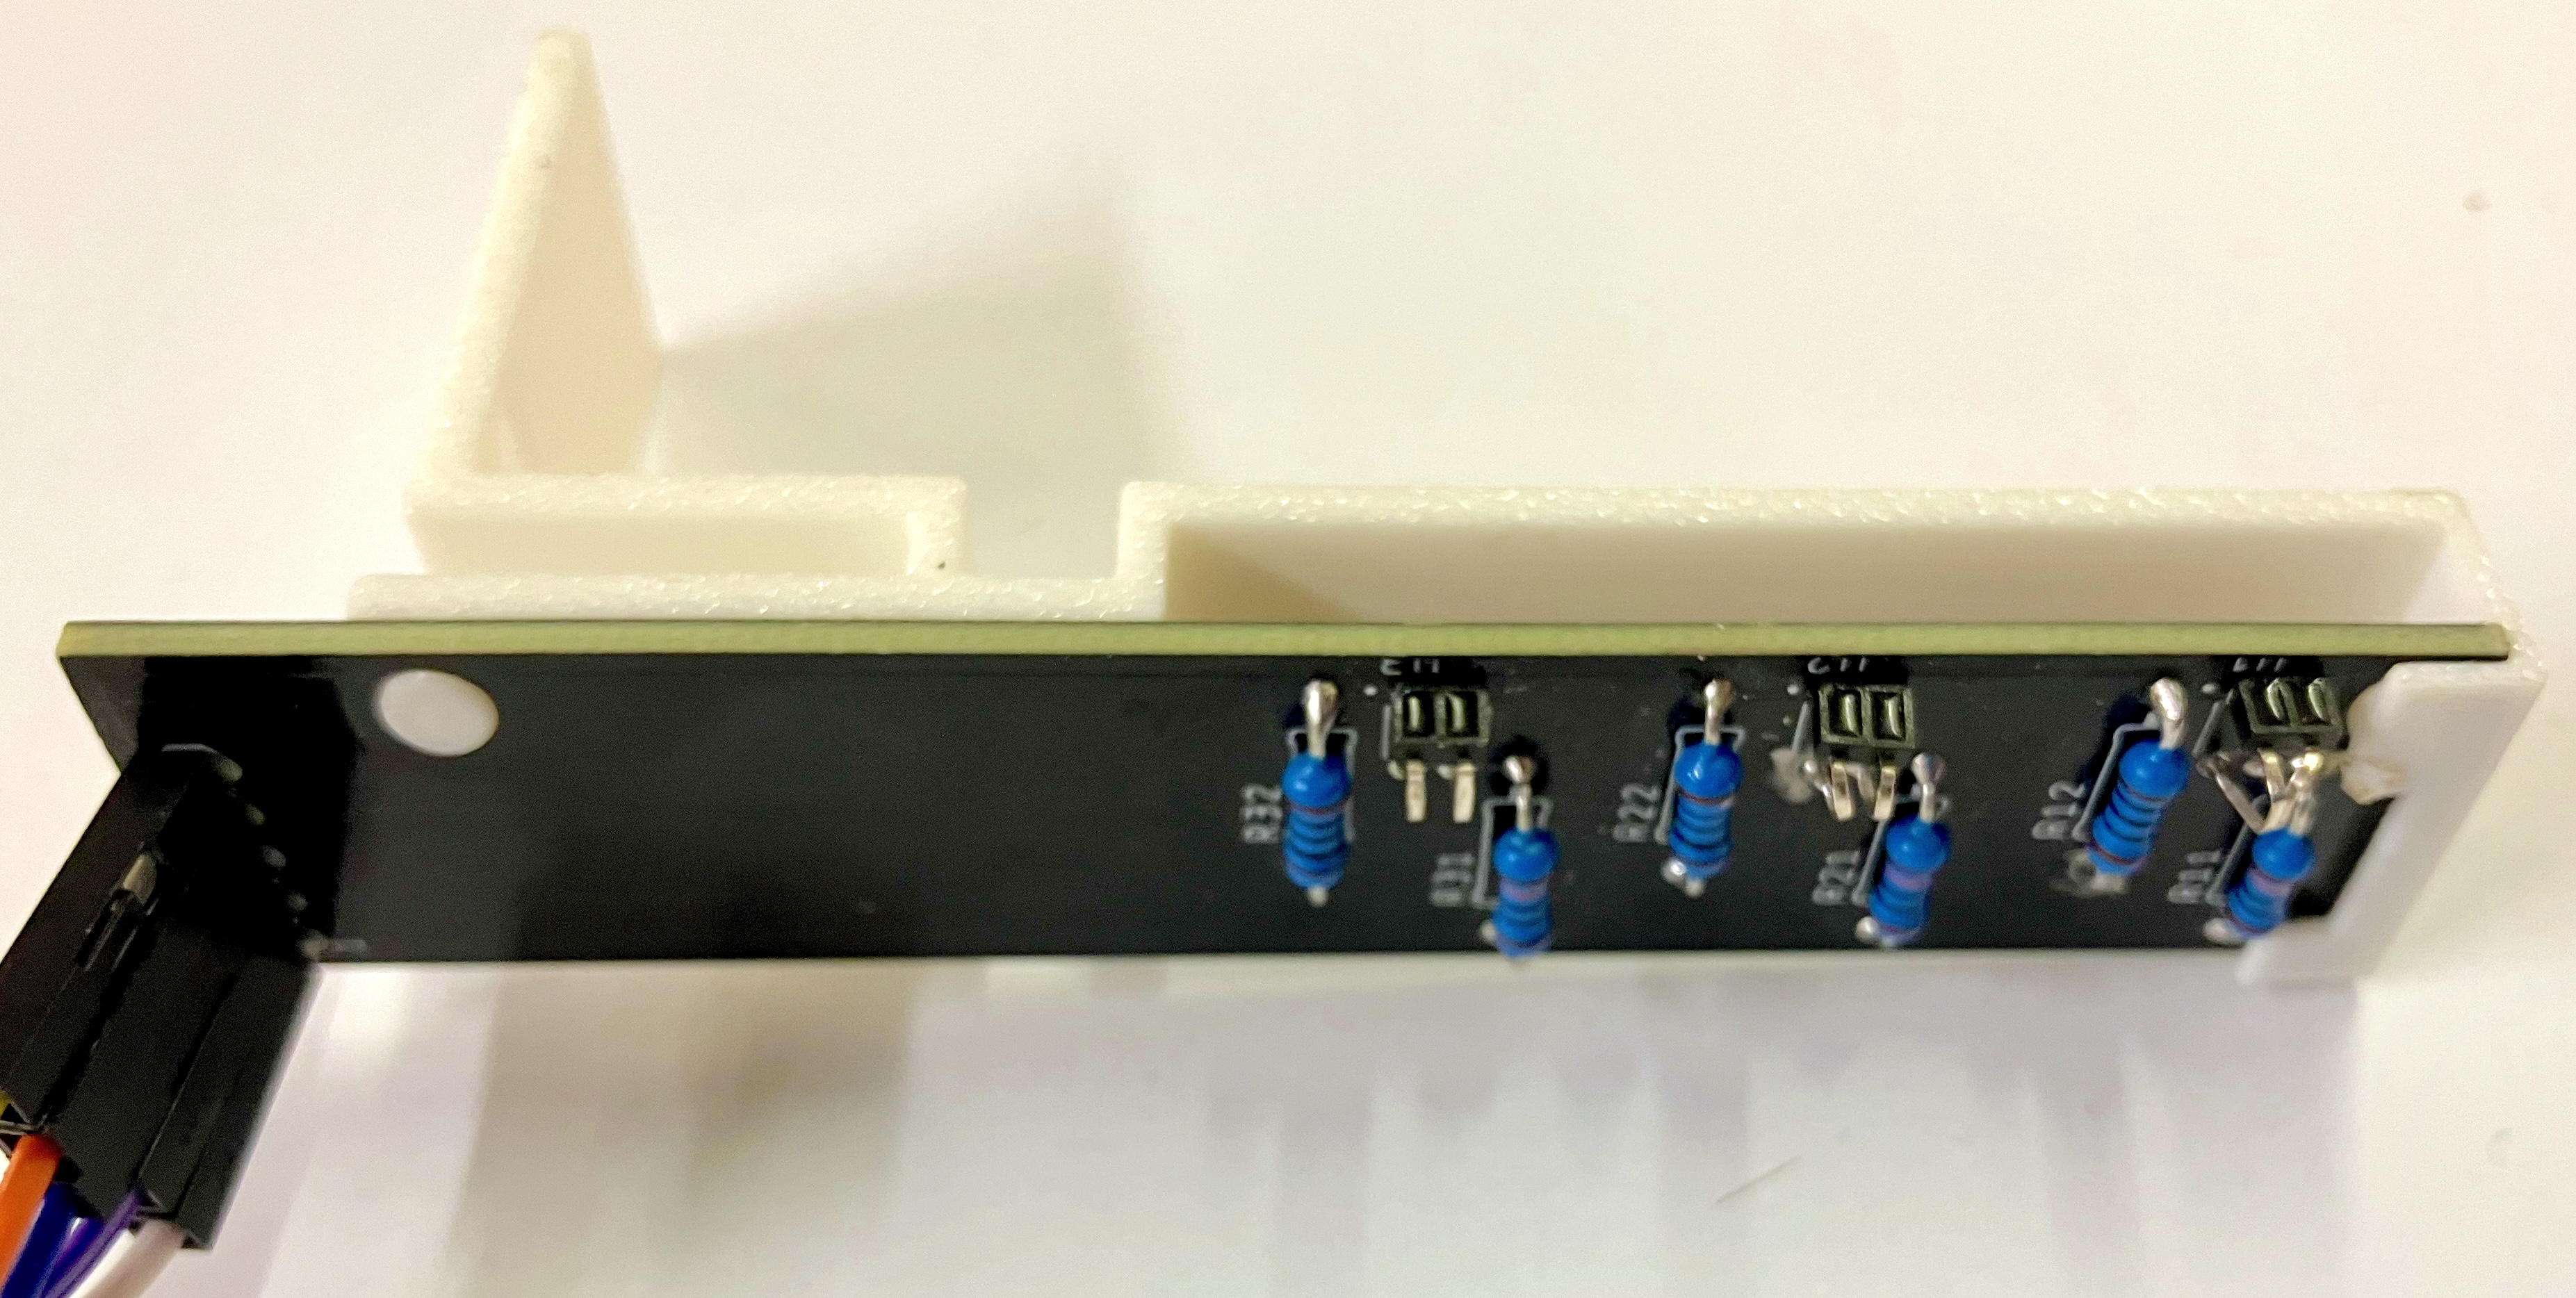
\includegraphics[width=0.3\linewidth]{img/prototype-mini-pcb-mount.jpeg}
    \caption{Prototype PCB attached to 3D printed adjustmet bracket.}
    \label{fig:prototype-pcb-mount}
\end{figure}

This would allow the PCB to be mounted to an adjustable 3D printed bracket which was fitted to the side of the wrestplank. The bracket was designed to allow adjustment in the distance between the sensor and the gradient tag. The intention was for the final PCB to mounted horizontally on the underside of the wrestplank. While assembling the prototype PCB, it was found that the optical sensor contacts were too fragile and could be easily broken in this process. An end-mount approach like that taken in \textcite{mcpherson_portable_2013} was attempted, but the short side of the jack body, at a width of 4.30 millimetres, presented a much smaller target than the keyboard keys. Slight deviations in sensor alignment resulted in drastic changes to the range of the output signal. Instead, the optical sensors would need to be soldered flush against the PCB, which would require the PCB to orientate vertically.

\begin{figure}
    \centering
    \includesvg[inkscapelatex=false,width=0.75\linewidth]{img/pcb-dual-sensor-board.svg} \\
    \includesvg[inkscapelatex=false,width=0.75\linewidth]{img/pcb-dual-sensor-board-traces.svg}
    \caption{Vertically orientated prototype sensor PCB schematic (Top) and traces (Bottom).}
    \label{fig:dual-pcb}
\end{figure}

The prototype PCB was redesigned in a new vertical orientation (Figure~\ref{fig:dual-pcb}) in which the sensors layout were doubled. The 3-key model action had limited space and only allowed wiring from a single direction. Doubling the sensors in the design allowed the circuit to wired two different ways to accommodate the change in orientation for the front and rear registers while also keeping the same vertical positioning. This was done to minimise the differences in signal ranges and avoid the necessity of printing two offset gradients or fabricating two different PCBs. The final full-scale interface would have enough internal space to accommodate routing on either side of the registers.   A two-piece 3D printed bracket held the PCB in a vertical orientation while also allowing for broad adjustments of the gap between the sensors and the surface.


\section{Mark 1}

The first, complete version of the interface was designed for exhibition at San Colombano, herein referred to as Mark 1.
A modular approach was taken during the design and fabrication of Mark 1. Development was divided into the mechanical hardware, electronics, and audio software. The electronics were further divided as hardware and firmware. This modular approach allowed construction to begin on the mechanical interface while prototyping still continued. Concurrent development allowed for changes or limitations in one module could be accounted for in the others. 

The target audience for the interface is visitors to the
museum, who would interact with instrument if it were working order. The
keyboard, which museum visitors can use without special permission, presents
two choirs of muted strings and can generate MIDI messages. 
The keyboard targets all visitors to the museum, regardless of playing ability,
and can be used without special permission. Jacks that pluck two choirs of muted
strings, across 49-keys, are used to generate MIDI messages that are sent to a
connected computer for audio synthesis. The interface is presently linked to a
commercial software sampler; however, the ultimate aim is to make the sound of
instruments in the collection that can no longer be maintained in playable
condition accessible. Museum visitors are invited to play the interface and
listen through a pair of headphones. This work outlines the technological
aspects of the interface's construction and offers reflections on its role
within the Tagliavini Collection and potential application within the
wider musical instrument museum context. 
The intended use of the keyboard through meaningful interaction with a museum exhibit is where the novelty of this work lies, rather
than solely in its technological development.

\subsection{Mechanical Hardware}

The mechanical hardware and its design constraints were co-authored with luthier Roberto Livi and curator of San Colombano Catalina Vicens using the design constraints in Section~\ref{sec:design-constraints}. After the designs had been finalised, the NEMUS project commissioned Roberto Livi to build the hardware at his workshop in Pesaro. The rectangular frame deviates from the traditional logarithmic (Figure \ref{fig:compare}) form as the interface needed to be compact enough not
to compromise space for exhibition of the permanent display.

\begin{figure}
    \centering
    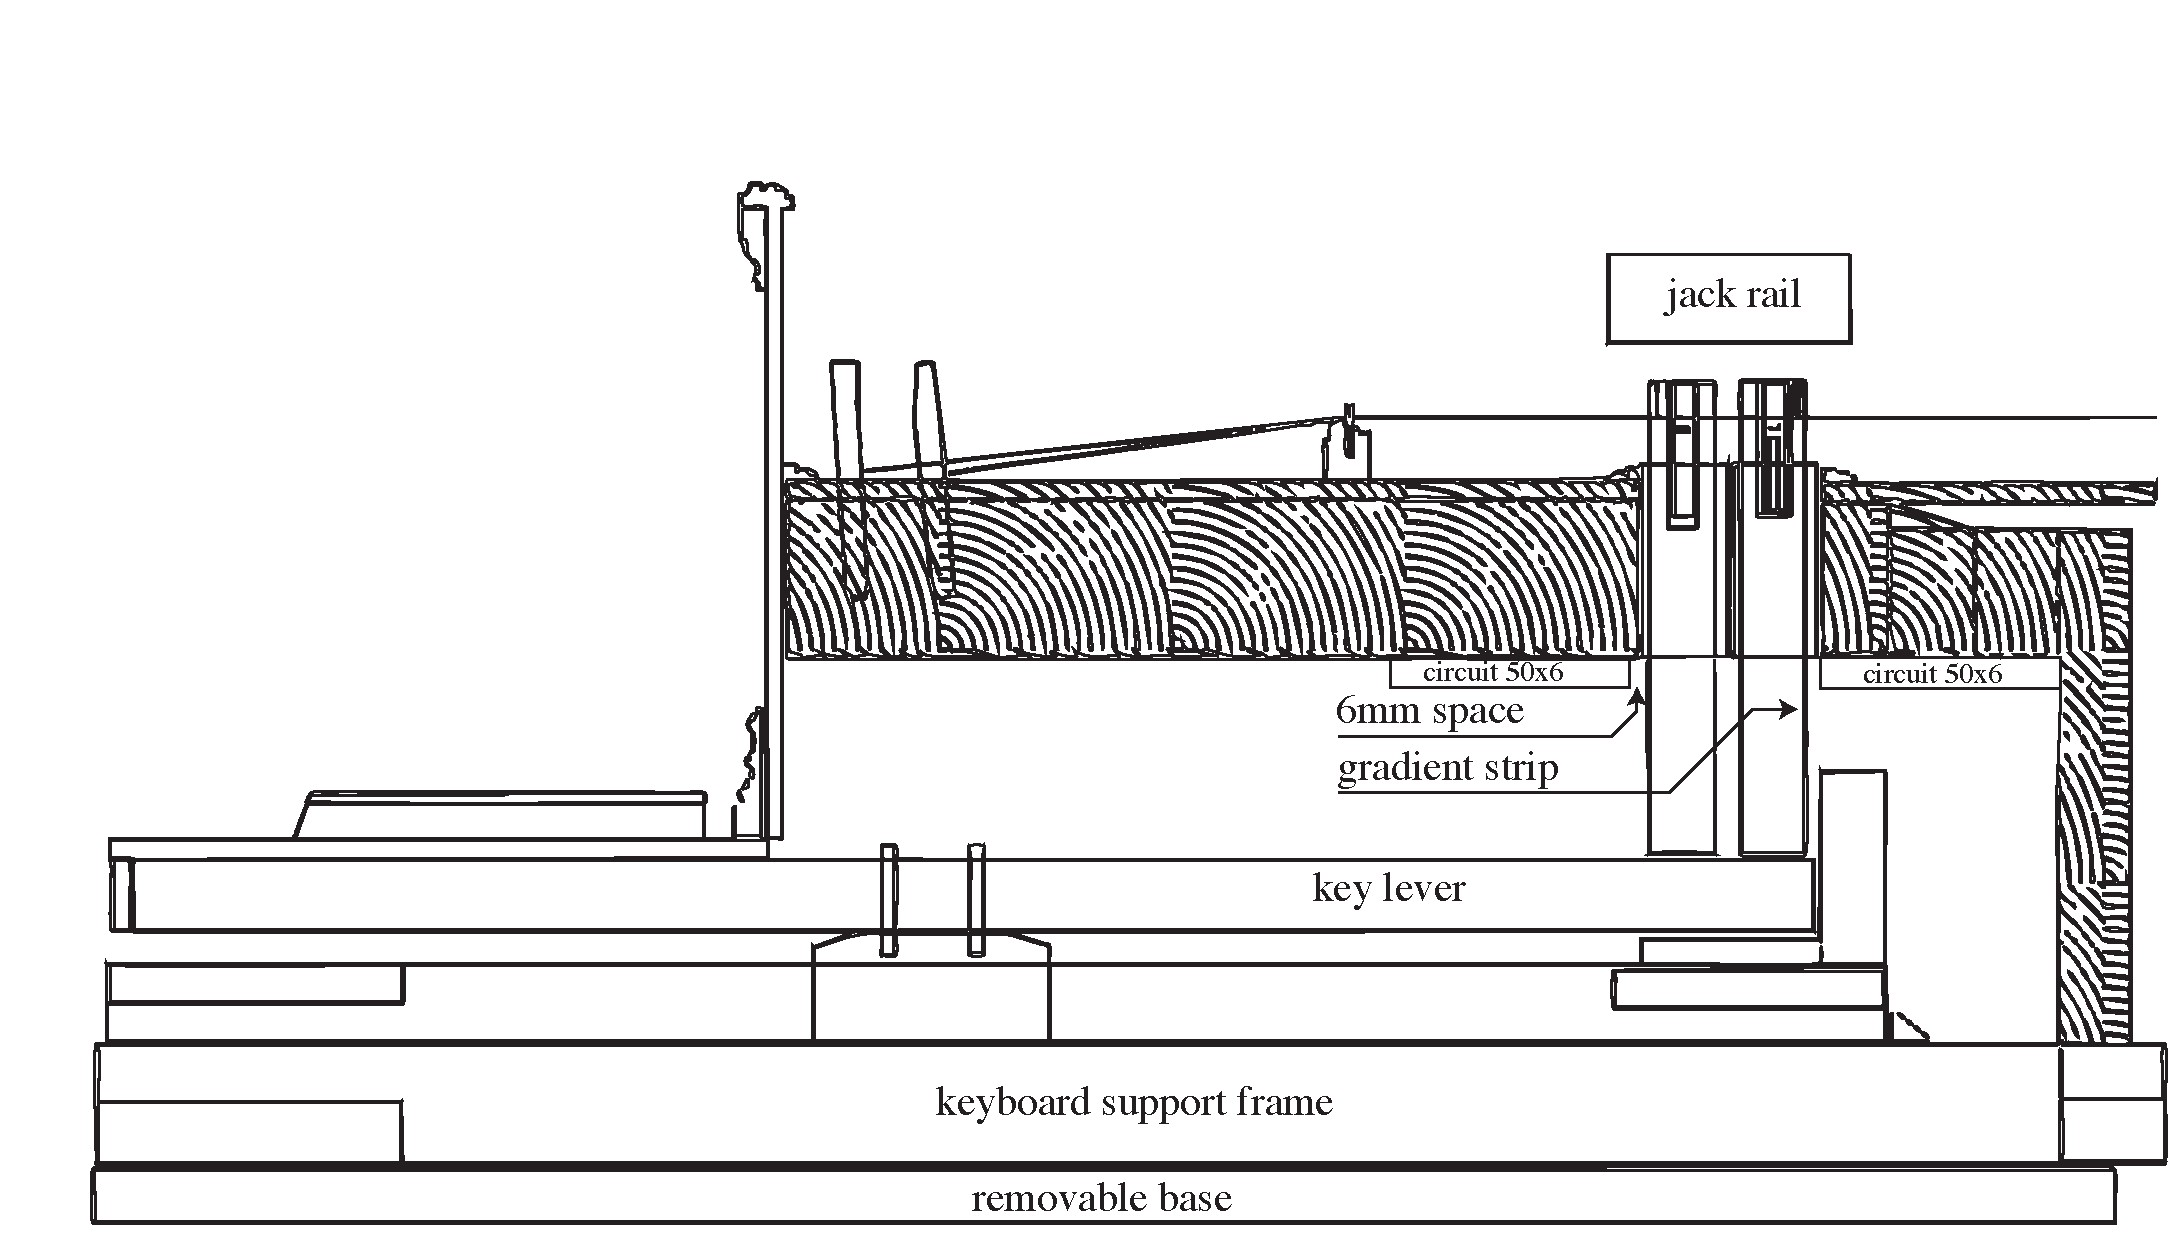
\includegraphics[width=1\linewidth]{img/drawing-mark-1-model-cross-section.pdf}
    \caption{Cross-section of keyboard mechanics by Roberto Livi. Not the original design was to accommodate a horizontal circuit board of dimensions 50mm by 6mm.}
    \label{fig:mark-1-cs}
\end{figure}

An internal cavity with excess space was stipulated as part of the design in order to provide flexibility with the potential PCB size. The final dimensions in the design also dictated an upper limit to the internal footprint of electronics (Figure~\ref{fig:mark-1-cs}).

The keyboard was designed to replicate the tactile sensations and aesthetics of
a historical Italian harpsichord. Traditional materials were used,
including walnut for the wrest plank, chestnut for the key levers, boxwood and
ebony for key covers, and cypress for the case and soundboard. The 98 jacks were
made from beech, fitted with brass springs and natural seagull feather plectra.
The design was inspired by the 1547 Alessandro Trasuntino harpsichord at
the San Colombano Museum, considered one of the first prototypes to have
been conceived with two sets of 8-foot strings. An exception was made for the
short octave --- the assigning of common keys in the first octave instead of a
chromatic scale --- typically found in Italian harpsichords, which was replaced
by a standard octave layout to more easily accommodate the interaction with
commercial samplers. 

\begin{figure}
    \centering
    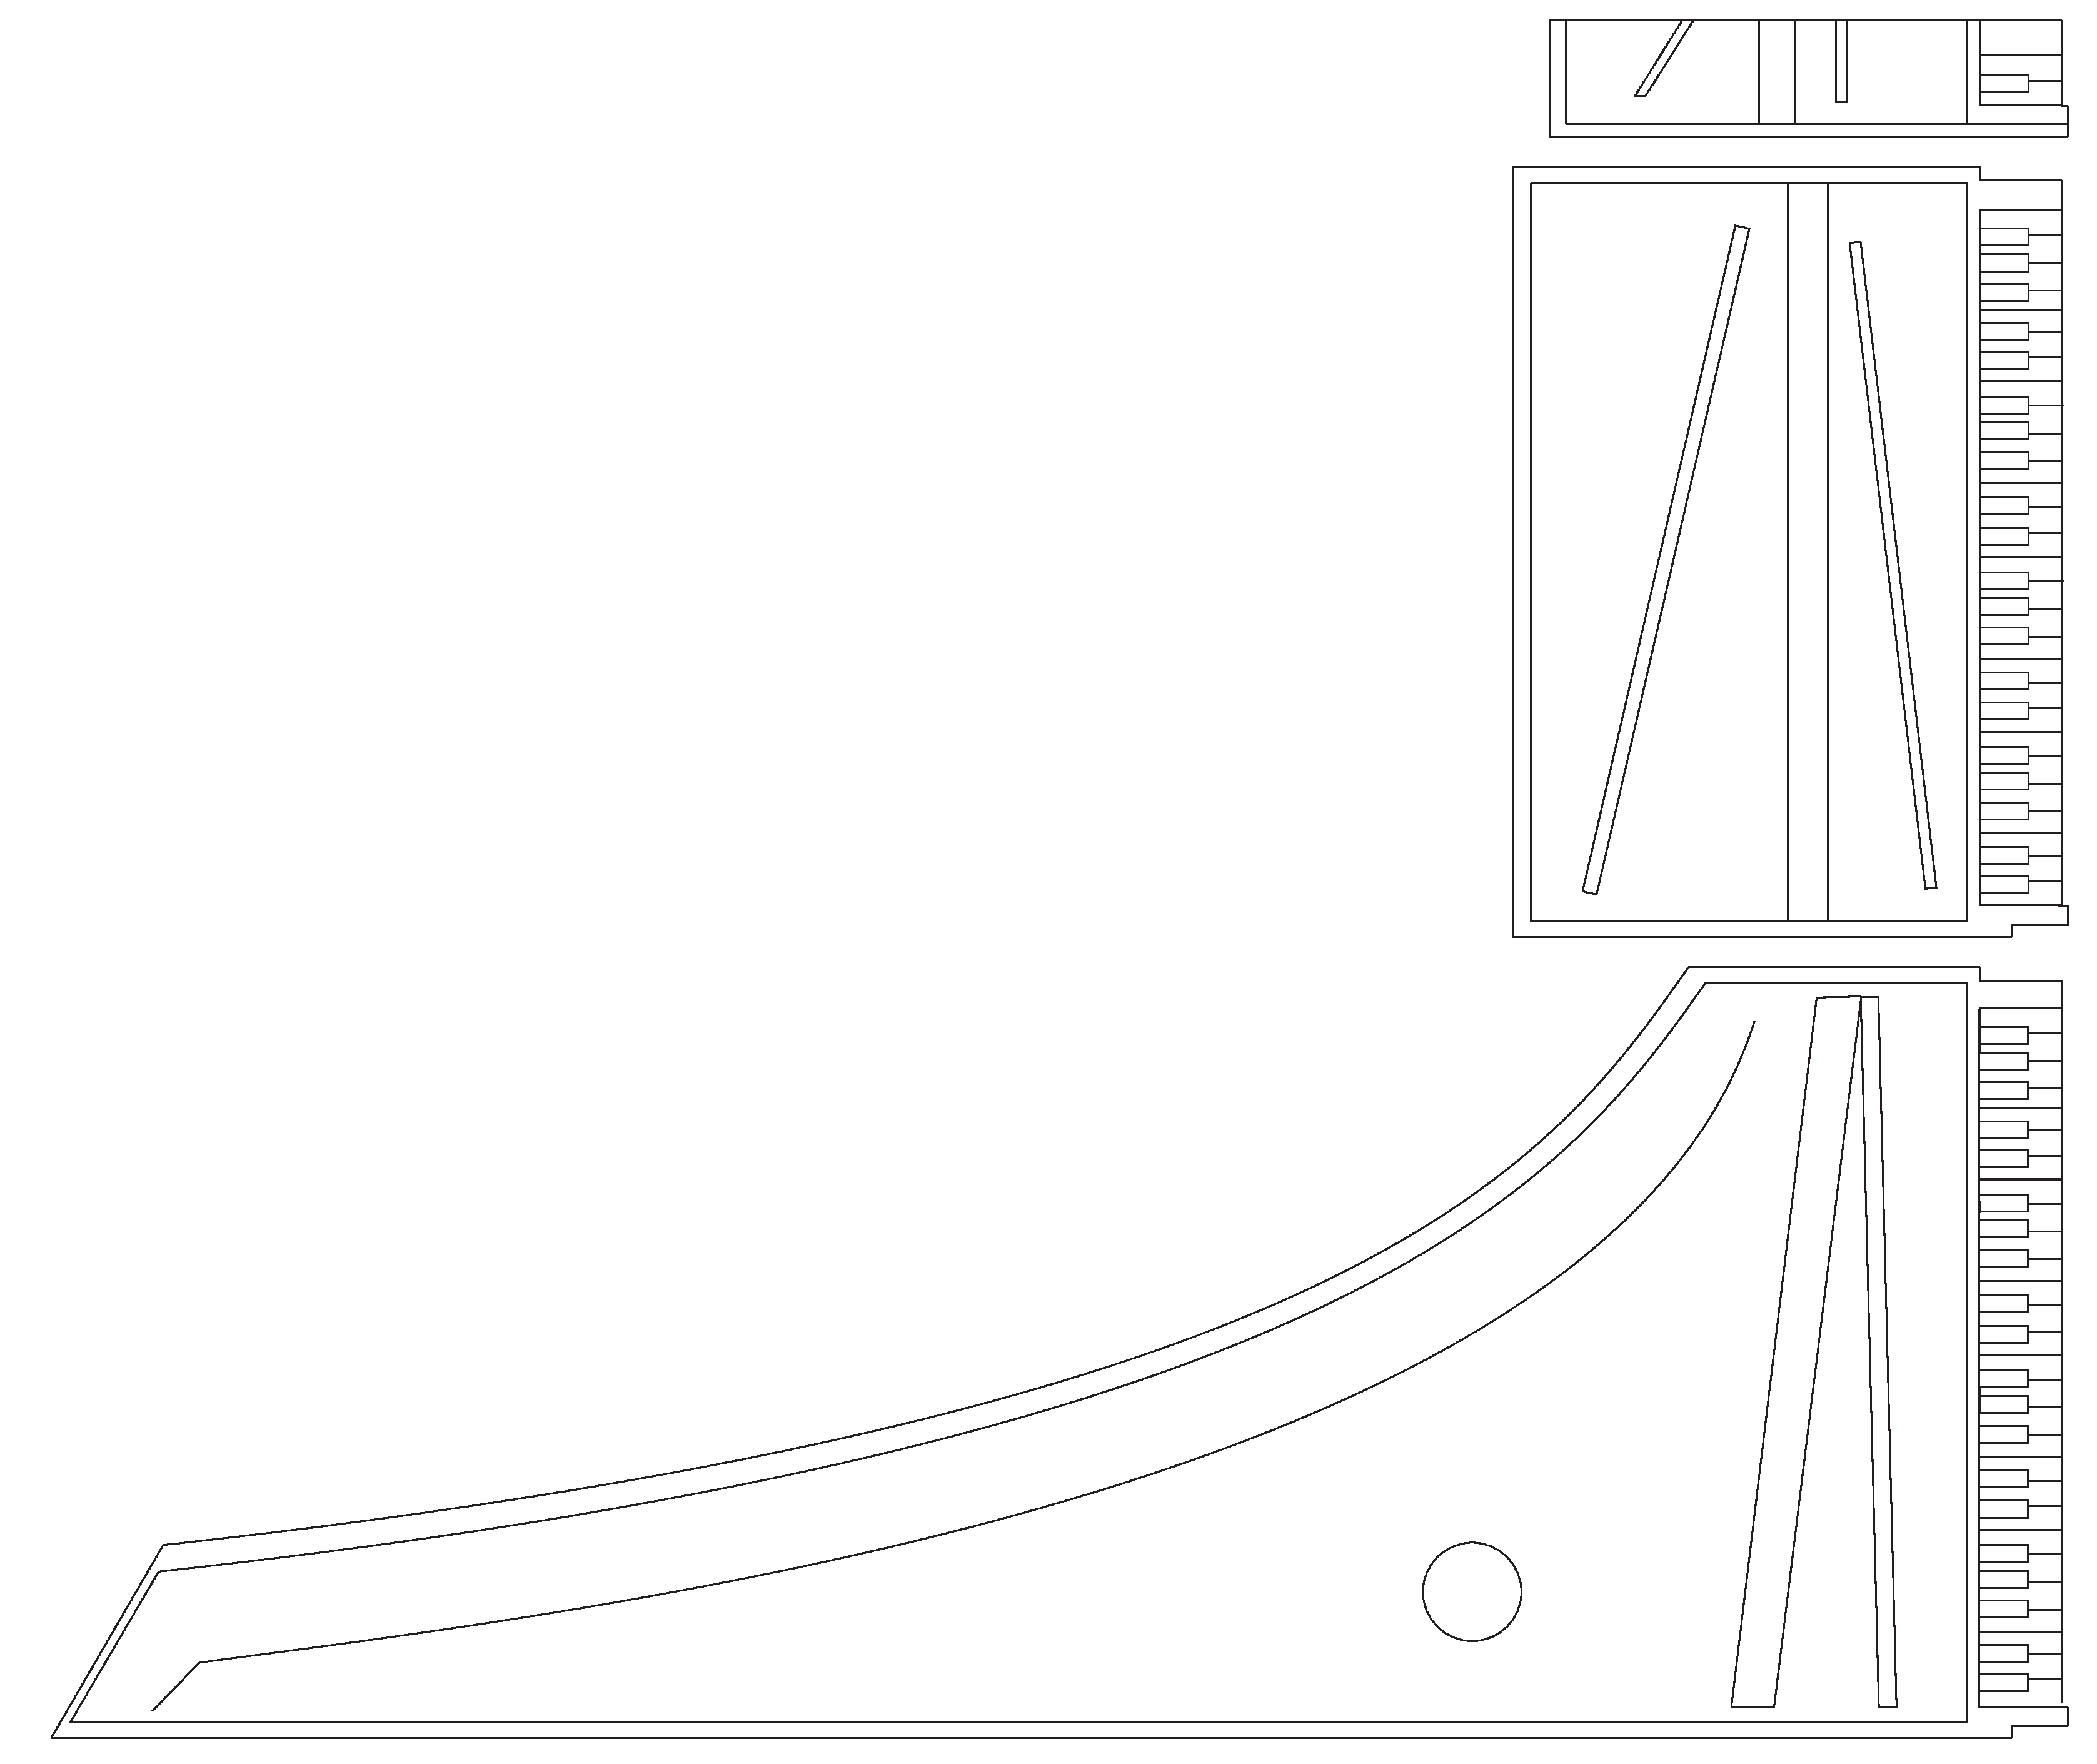
\includegraphics[width=0.75\linewidth,angle=270]{img/drawing-all_comparison-90.pdf}
    \caption{Scale comparison: (from left to right) the 1547 Trasuntino, 49-key `Mark 1' model, and the 3-key prototype. The Trasuntino provides an example of the `logarithmic' form of a traditional harpsichord.}
    \label{fig:compare}
\end{figure}

The rectangular poplar frame also deviates from the traditional logarithmic
(Figure \ref{fig:compare}) form to allow for the installation of the
electronic sensors, as visible in Figure \ref{fig:mark-1-bottom}, without
compromising the visual or tactile authenticity. Two string choirs, crafted from
yellow brass wire and anchored with wrought iron pins, were tensioned to
replicate authentic plucking resistance. Felt strips were added to dampen
vibrations. The result is an interface with the mechanical action of
keys that preserves a real harpsichord's haptic qualities.

\begin{figure}
    \centering    
    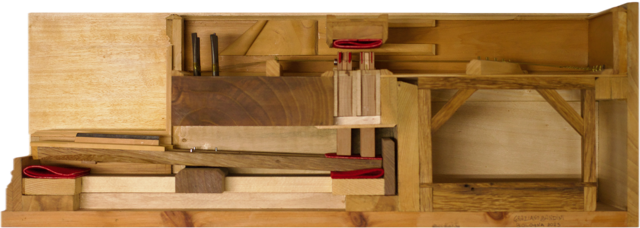
\includegraphics[width=\linewidth]{img/3-key-side.png}
    \caption{ 3-Key Model Harpsichord Mechanism.}
    \label{fig:3key}
\end{figure}



% A common piece of advice for those purchasing a guitar is for them to wear a blindfold as they try instruments. This is to avoid the buyer being influenced by the `look' of the instrument over the sound or the feel to the detriment to their comfort.

\subsection{Electronic Components}

This section covers the electronics components utilised in the final circuit design, their purpose and reasons behind their choice.

\subsubsection{Microcontroller}\label{nano-ble}

All the electronic components in the system terminate at a microcontroller, whose job is to convert analogue signals to digital data, and control the other components in the system. Microcontroller are re-programmable, which allow for easy iterative development and algorithmic control over other electronic components. For microcontroller, an Arduino Nano 33 BLE (Bluetooth Low Energy) was chosen as the final design, hereafter referred to as simply the Nano BLE. The Arudino Nano line of microcontrollers have a standardised form factor, which is to say they have a standard size and pin layout. Since it was unclear what the computational and functional requirements would be for the microcontroller, standardised form allowed for the testing of multiple models and chipsets. For the prototyping stage, an Arduino Nano 33 IoT was used as the initial microcontroller given its ready availability. When scaling the final sensor concept, it was found that the Nano 33 IoT had limitation on its analogue-to-digital converter (ADC) input channels four and five \cite{arduino_nano33iot_2025}, limiting the total number of input channels to just six. This limitation in input channels would have a great impact in the layout of the rest of the circuit. The Nano BLE, which had all eight ADC channels available, was therefore swapped in of the Nano 33 IoT with the firmware and circuitry remaining the same.

The Arduino Nano models also provided native-USB functionality, which allowed the microcontroller to be programmed as a hardware USB MIDI device directly. In addition, the Nano BLE allowed a fallback of using the MIDI BLE protocol, should there be any difficulty in connecting the microcontroller to the computer used for audio synthesis. A further benefit of the Nano BLE was its The Nano 33 BLE 12-bit digital-to-analogue converter (DAC), which provided a contingency should the default 10-bit not be sensitive enough for the signal from the sensors.

% A rough performance test was later carried out using an STM32 NUCLEO-L031K6, a
% Nano ESP32 and the BLE. The Nano 33 BLE was found to be more performative. To
% execute a single sensor read cycle of the firmware the STM32 took 40ms, and both
% the Nano ESP32 and Nano 33 BLE required 11ms on average. The Nano ESP32 had high
% variability so it was decided to continue with the Nano 33 BLE. 

\subsubsection{Non-Volatile Memory}\label{eeprom-nvram-fram} 

The signal values for the jack pluck and release points needed to be calibrated and stored so that they had permanence between power cycles. Adjusting the threshold values through firmware would not have been flexible or practical, therefore a form of non-volatile memory (NVM) was required.  The Nano BLE did not provide any direct NVM and what memory was available would be lost during re-programming.

Instead a Fujitsu MB85RS64 Ferroelectric RAM (FRAM) module was chosen. Two standard communication protocols are available on the Nano for communicating with other odules: Inter-Integrated Circuit I\textsuperscript{2}C and  Serial Peripheral Interface (SPI). The pins associated with the  I\textsuperscript{2}C interface were used for the sensor output ADC, which left the only the SPI interface available. The MB85RS64 was chosen for its SPI support and relatively low power consumption compared to other NVM technology \cite{fujitsu_fram_2011}.

Alternatives to the FRAM were available. The problem could also have been addressed with the use of an SD card and reader. An SD card would have provided a means to edit calibration values away from the Arduino. The position of the controller board within the interface did not permit easy access. Reliability and speed of executing the calibration process was preferred over storage capacity of an SD card. Additionally, calibration values could have been stored on the audio synthesis computer and communicated to Nano BLE directly. This would have necessitated an extra step in the setup process and a point failure. This approach would have made the interface less portable, limiting connection to audio synthesis devices on which additional software could be installed, thus undoing the portability that the MIDI standard provided.


\subsubsection{RGB LEDs}

\begin{figure}
    \centering
     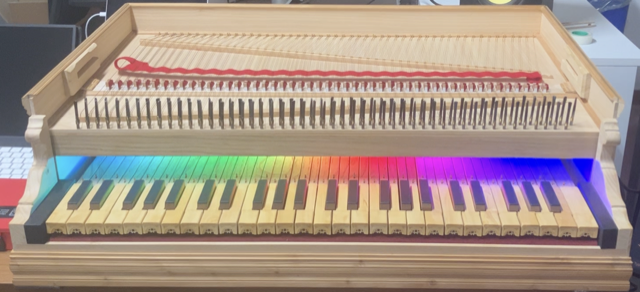
\includegraphics[width=0.66\linewidth]{img/mark-1-leds.png}
    \caption{Mark 1 demonstrating addressable RGB LED array.}
    \label{fig:mark1-leds}
\end{figure}

With the prototype keyboard there were at most six jacks requiring calibration. Moving to the 98 jacks of the Mark 1 interface introduced what could be referred to as `problems of scale', problems that arise only in the scaling up of a design. One such problem of scale was how the user keeps track or identifies which key is currently calibrated. To assist the user, addressable RGB LEDs were added to the design. The LEDs are aligned with the sensors and are controlled programmatically via a pulse width modulation (PWM) signal and are addressable individually. This allows for an LED to illuminated in front of a key that is being calibrated to aid identification.
The colour can also be controller (Figure~\ref{fig:mark1-leds}) which allows for visual feedback on both interface and key states. This allowed for visual identification if a sensor had fallen out of an expected range or if a key had still used its default threshold value and was still to be calibrated.

A separate driver such as the \texttt{TLC5940} used in \textcite{mcpherson_portable_2013} added
complexity to assembling and were avoid in favour of addressable LEDs with
integrated driver and shared data line. One limitation to this approach is should any LED in chain fail, the fault will prevent all subsequent LEDs from illuminating.
An individual PWM driver per PCB avoids cascading failure, but would have add 
complexity in the assembly process as they are typically in an SMD for factor.
As covered in Section~\ref{}, THT components were preferred in the initial design stages to allow for easier manual assembly and alteration of wiring and components.
In the event of a failure with other components, the the solution was to replace the faulty PCB. As such, failing LEDs did not present a great enough problem to justify a design change.
Furthermore, the LEDs were to included to aid debugging and calibration, there failure would not otherwise effect the operation of the interface. The LEDs would also be hidden behind the name board of the exhibition interface during standard operation.

\subsubsection{Multiplexer}

The number of available analogue-to-digital converter (ADC) channels  on the Arduino is limited to eight. For the prototype, sensors outputs were connected directly to the available ADCs.
One of the first a `problems of scale', introduced when expanding from six jacks of the prototype model to the Mark 1, was how to accommodate 98 optical sensors. To overcome the Arduino's ADC limitation, a \texttt{CD4051BE} Texas Instruments multiplexer was introduced.  A multiplexer (multiplexor, MUX) a circuit that routes a common pin to one of several inputs or output. The MUX would provide a means to connect multiple sensor output signals to a single ADC pin on the Arduino. Available GPIO pins on the Arduino allowed for programmatic control of signal routing. This is the same way in with the ADCs themselves are routed on the Arduino \cite{nordic_nrf52840_2025}, meaning there is a cascade of two mux circuits. An 8-channel multiplexer was used in order to mitigate the problems typically associated with cascading multiplexers, such as increased signal settle time and increased noise. The sensor outputs were then divided between two microcontrollers.  Seven of the available eight channels on the \texttt{CD4051BE} were used, which provided a clean division of seven sensors per sensor board with seven sensor boards to cover 49 jacks in a register. In total, 14 sensor boards and two controller boards were installed. Details on the sensor and controller boards are given in the next section.

\subsection{Printed Circuit Boards}

To ensure stable connection, reduce the footprint of the circuit and fix the pitch spacing of the sensors to match the jacks, two PCBs were designed: the sensor board and the controller board.

Figure \ref{fig:system-block-diagram} shows a block diagram of the finalised
electronics setup, showing the connectivity between the sensor boards and the controller board on a macro level. 

\begin{figure}
    \centering
    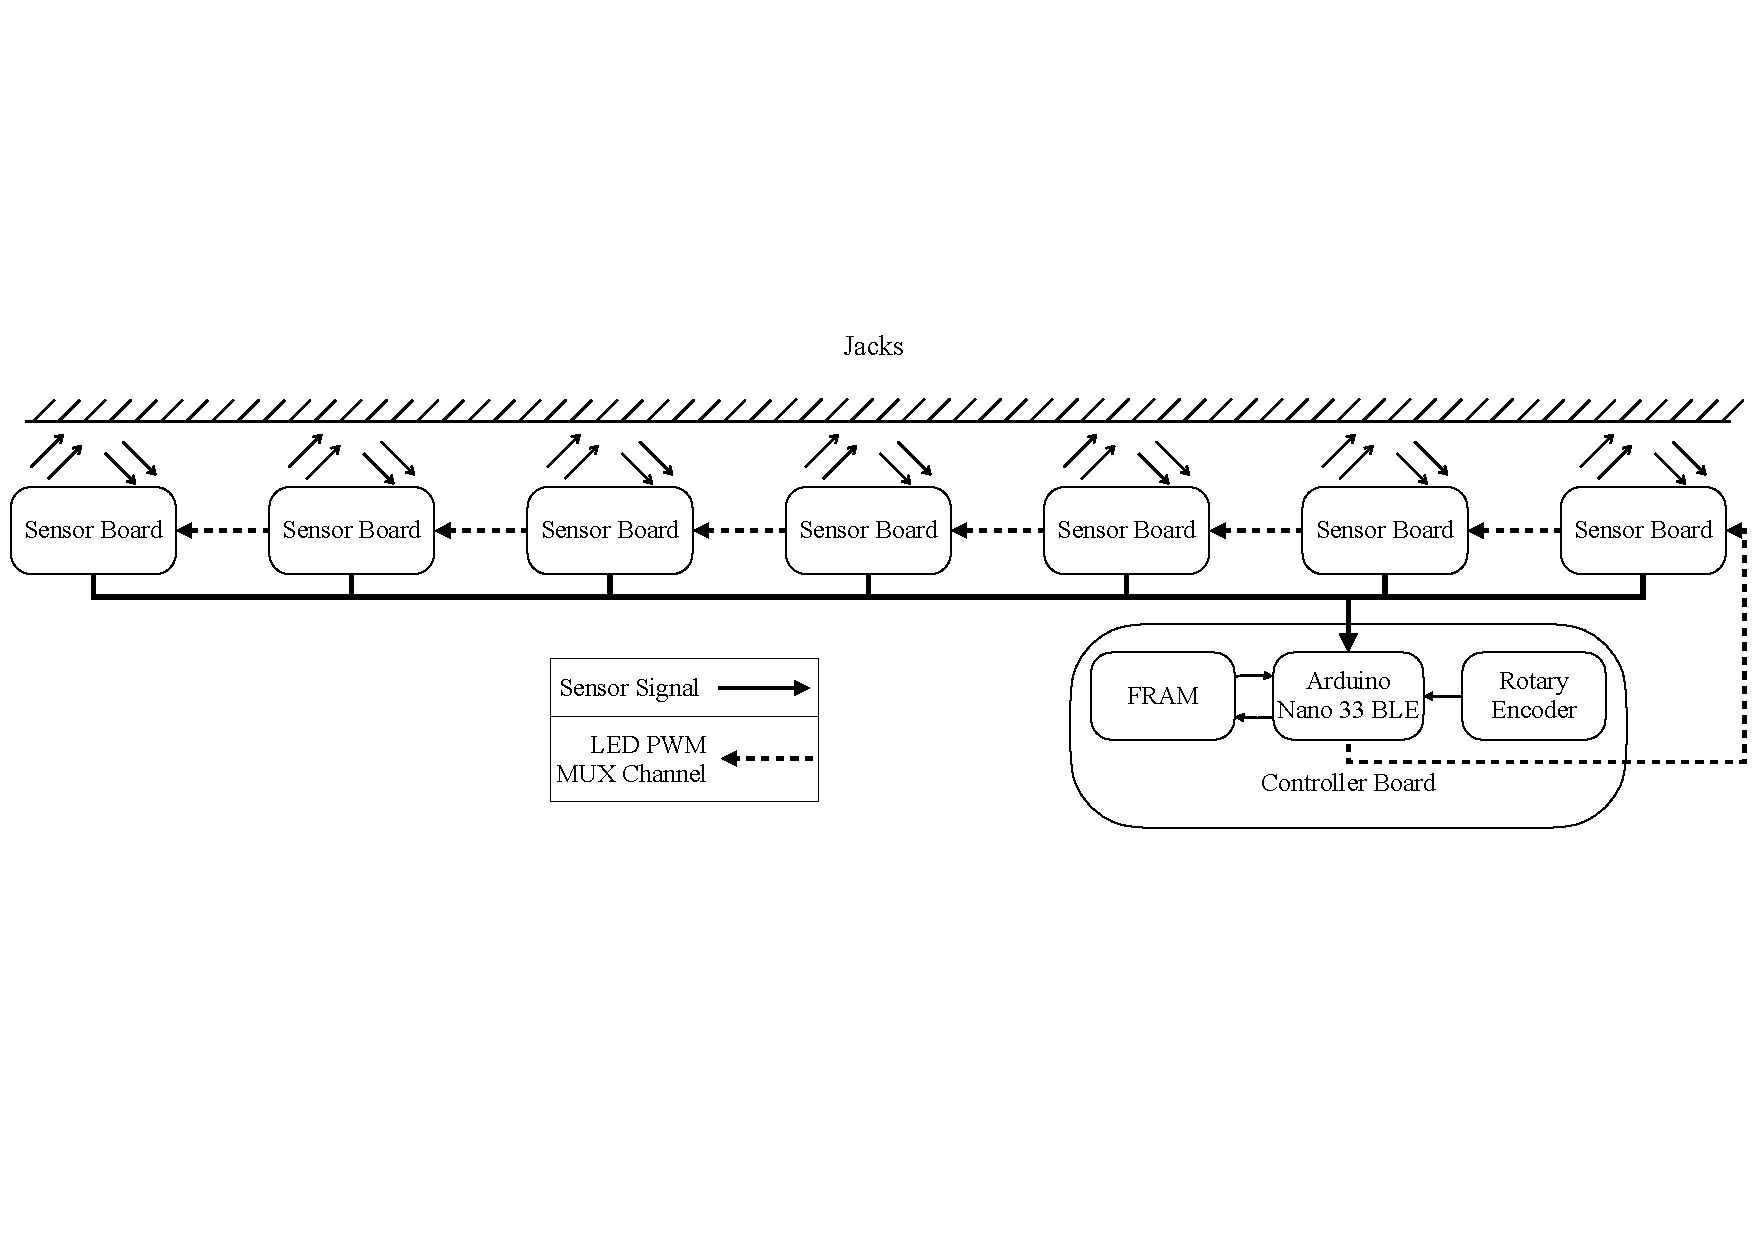
\includegraphics[width=\linewidth]{img/block-diagram-2.pdf}
    \caption{Block diagram of PCB connections. A separate sensor signal is routed to the Arduino. LED and multiplexer (MUX) controls signal are daisy-chained through each sensor PCB.}
    \label{fig:system-block-diagram}
\end{figure}

\subsubsection{Sensor Board}

The sensor board contains components required for the measurement of vertical jack displacement. Dividing the sensors across multiple boards reduced manufacturing costs, allowed for easier installation and provided some room for adjustment in both the distance between sensors and the surface but also the centre point to the corresponding seven jacks. Trace length between the output signal of the sensor and the MUX channel were kept as short as possible to minimise noise. Each sensor board  contained the following components:

\begin{itemize}
    \item 7 QRE1113 optical sensors.
    \item 7 100 $\Omega$ resistors and 7 10 k$\Omega$ resistors (later reduced
    to one resistor per board).
    \item 1 Texas Instruments \texttt{CD4051BE} multiplexer for signal aggregation.
    \item 7 WS2812 RGB LEDs with integrated driver.
\end{itemize}

\begin{figure}
    \centering
    \includesvg[inkscapelatex=false, width=\linewidth]{img/pcb_sensor_schematic_v1.svg}            
        \caption{Mark 1 Sensor board schematic. `\texttt{D}' labels correspond to LEDs and `\texttt{Q}' labels are the optical sensors. `\texttt{C}' labels show connection to corresponding multiplexer channel. Connection labels point in the direction of current flow.}
    \label{fig:sensor-schematic-1}
\end{figure}

Figure~\ref{fig:sensor-schematic-1} shows the schematic for the Mark 1 Sensor board.
Of note are the optical sensor signal output routed through the multiplexer (\texttt{SIG}) which was wired separately to the controller board. This was in art to make space for a multiplexer interrupt control (\texttt{INT}) which was ultimately never used. For the Mark 1 a solution had not yet been found for allowing all signals to flow through the sensor boards. The \texttt{A}, \texttt{B}, and \texttt{C} lines in Figure~\ref{fig:sensor-schematic-1} correspond to the first second and third bits of the 3-bit multiplexer channel selection (Table~\ref{tab:mux-encoding}).

\begin{figure}
    \centering
    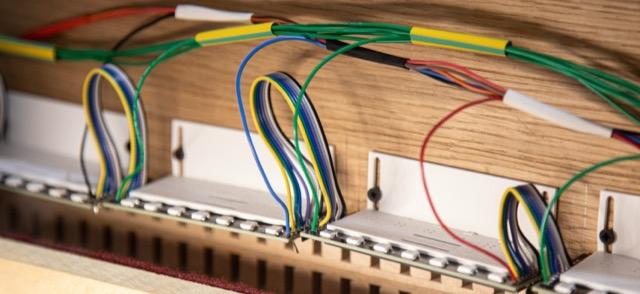
\includegraphics[width=0.75\linewidth]{img/mark-1-pcbs.jpg}
    \caption{Detail of sensor boards installed inside Mark 1. Cabling between sensor boards can be seen which corresponds to the \texttt{Input} and \texttt{Output} connectors in Figure~\ref{fig:sensor-schematic-1}. The multicoloured cable loom above the PCBs carries the \texttt{SIG} from each sensor board, while the green cabling is the unused interrupt channel that was ultimately connected to \texttt{GND}.}
    \label{fig:mark-1-pcbs}
\end{figure}

Ribbon cable was used solder the \texttt{Input} and \texttt{Ouput} of the sensor boards together. This was done prior to installation and the entire assembly was fitted as a single chain.
A separate cable for the output signal was taken from each PCB (Figure~\ref{fig:mark-1-pcbs}) which were collected in a separate cable loom and connected to a header on the controller board for easy routing to the analogue channels (Figure~\ref{fig:controller-schematic-1}).

The same style of 3D-printed baffles as used in the prototype were installed on the sensor boards to eliminate cross-talk between adjacent sensors, as per Figure \ref{fig:baffles}. 
These baffles, fabricated from dark-pigmented, matte PLA, ensured that infrared reflections from neighbouring jacks did not interfere with sensor readings. The baffles (Figure~\ref{fig:sensor-physical-pcbs}, alongside an adjustment plate and a vertical mount back plate, formed a three-part bracket assembly.
Visible in Figure~\ref{fig:mark-1-pcbs} is the adjustment brackets, which were used to both mount the sensor boards in a vertical orientation but also provide a means for broad adjustment of the distance between the sensor and gradients stickers. The three parts of the bracket are designed as a push fit so that they could be printed off-site, but assembled on on-site at the museum. The vertical backplate and adjustment plate fit together by means of a pressure fit dovetail join. Holes were placed on the sensor board design to accommodate such a bracket. Two 3mm holes are present on the sensor board allowing it to be sandwiched between between the back plate and the baffles. 

\begin{figure}
  \centering
  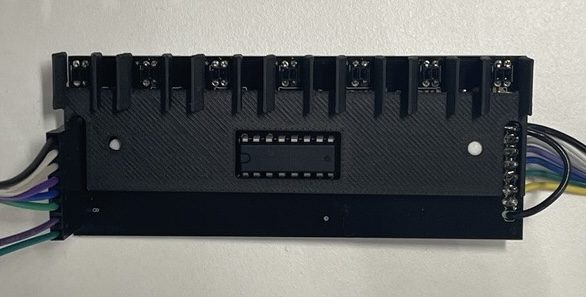
\includegraphics[width=0.6\linewidth,trim={0 1.5cm 0 1.5cm},clip]{img/sensor-board-w-baffles.jpeg}
    \\
  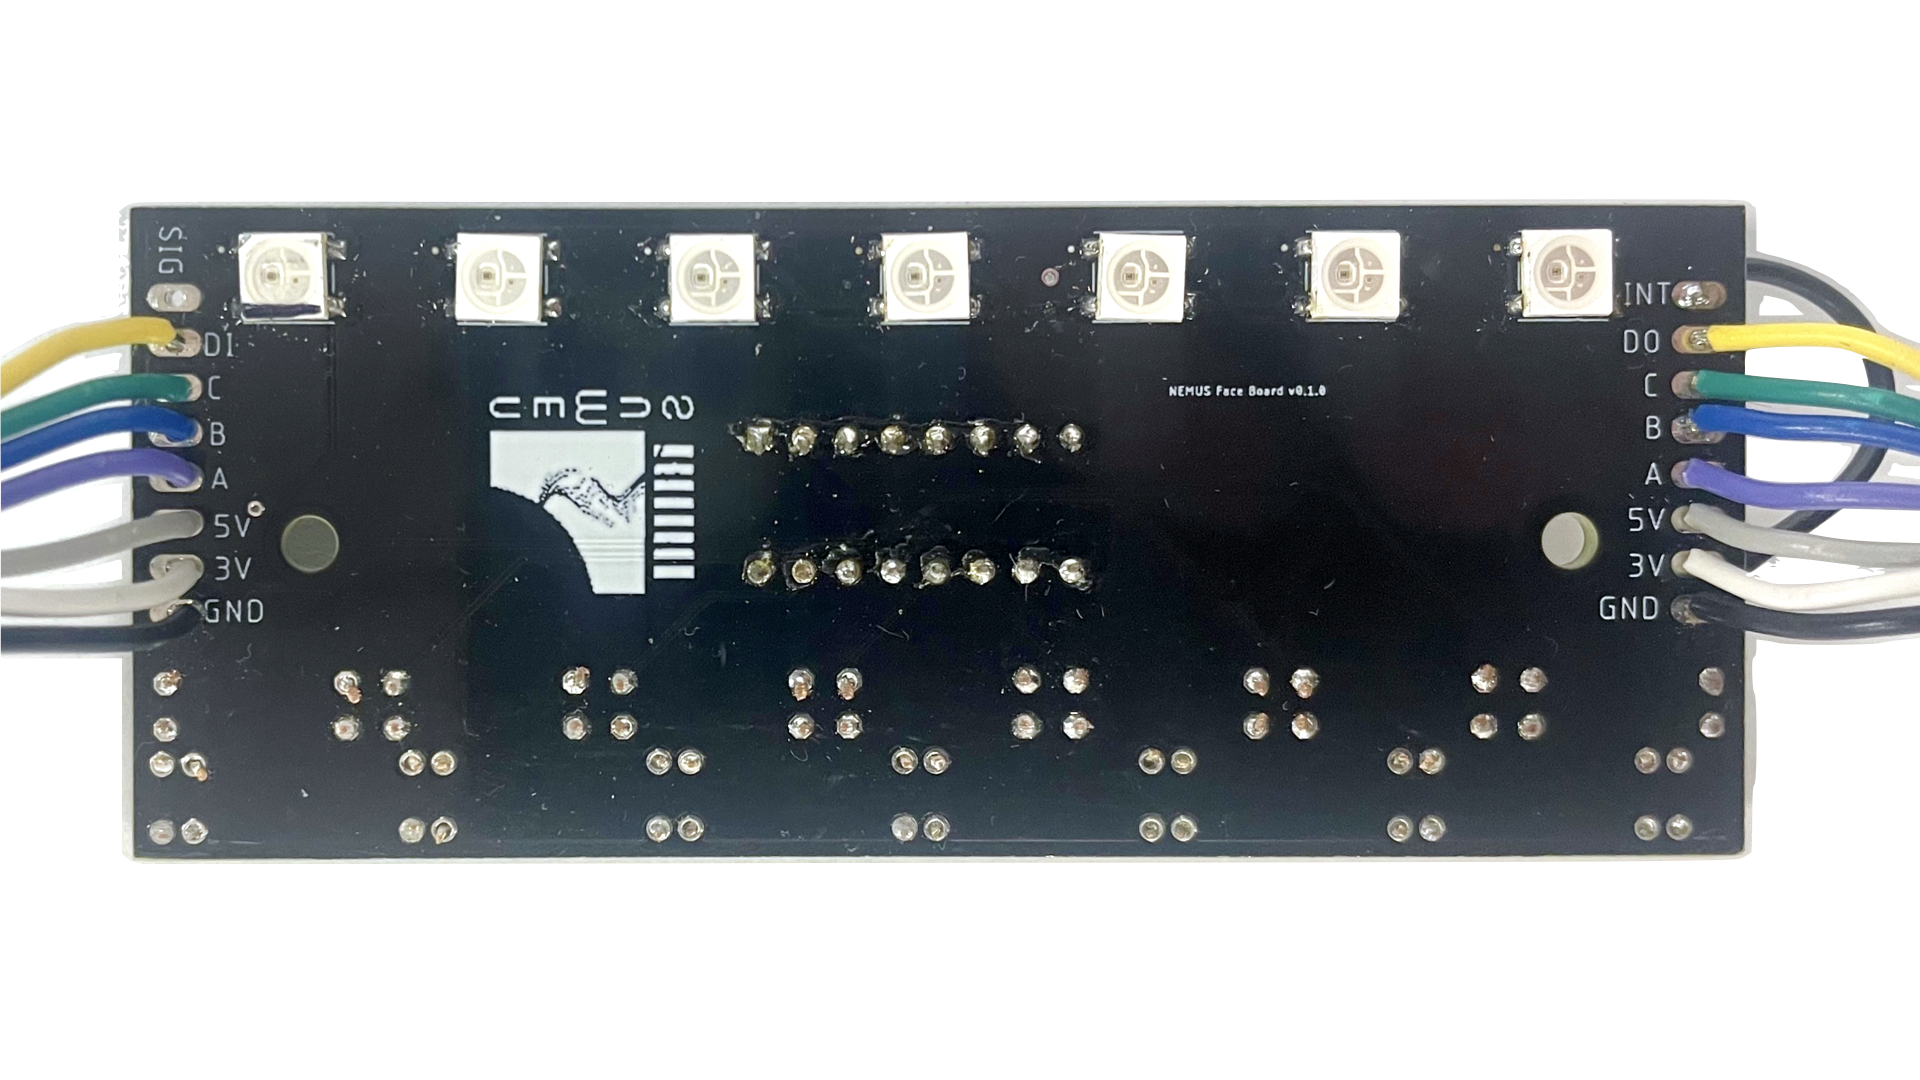
\includegraphics[width=0.6\linewidth,trim={4.45cm 4.5cm 5.25cm 4cm},clip]{img/sensor-board-reverse-side.png} 
  \caption{Sensor board showing the front side (top) and rear side (bottom) after ribbon cable installation but before \texttt{SIG} and \texttt{INT} terminals were connected.}
  \label{fig:sensor-physical-pcbs}
\end{figure}


\begin{figure}
    \centering
    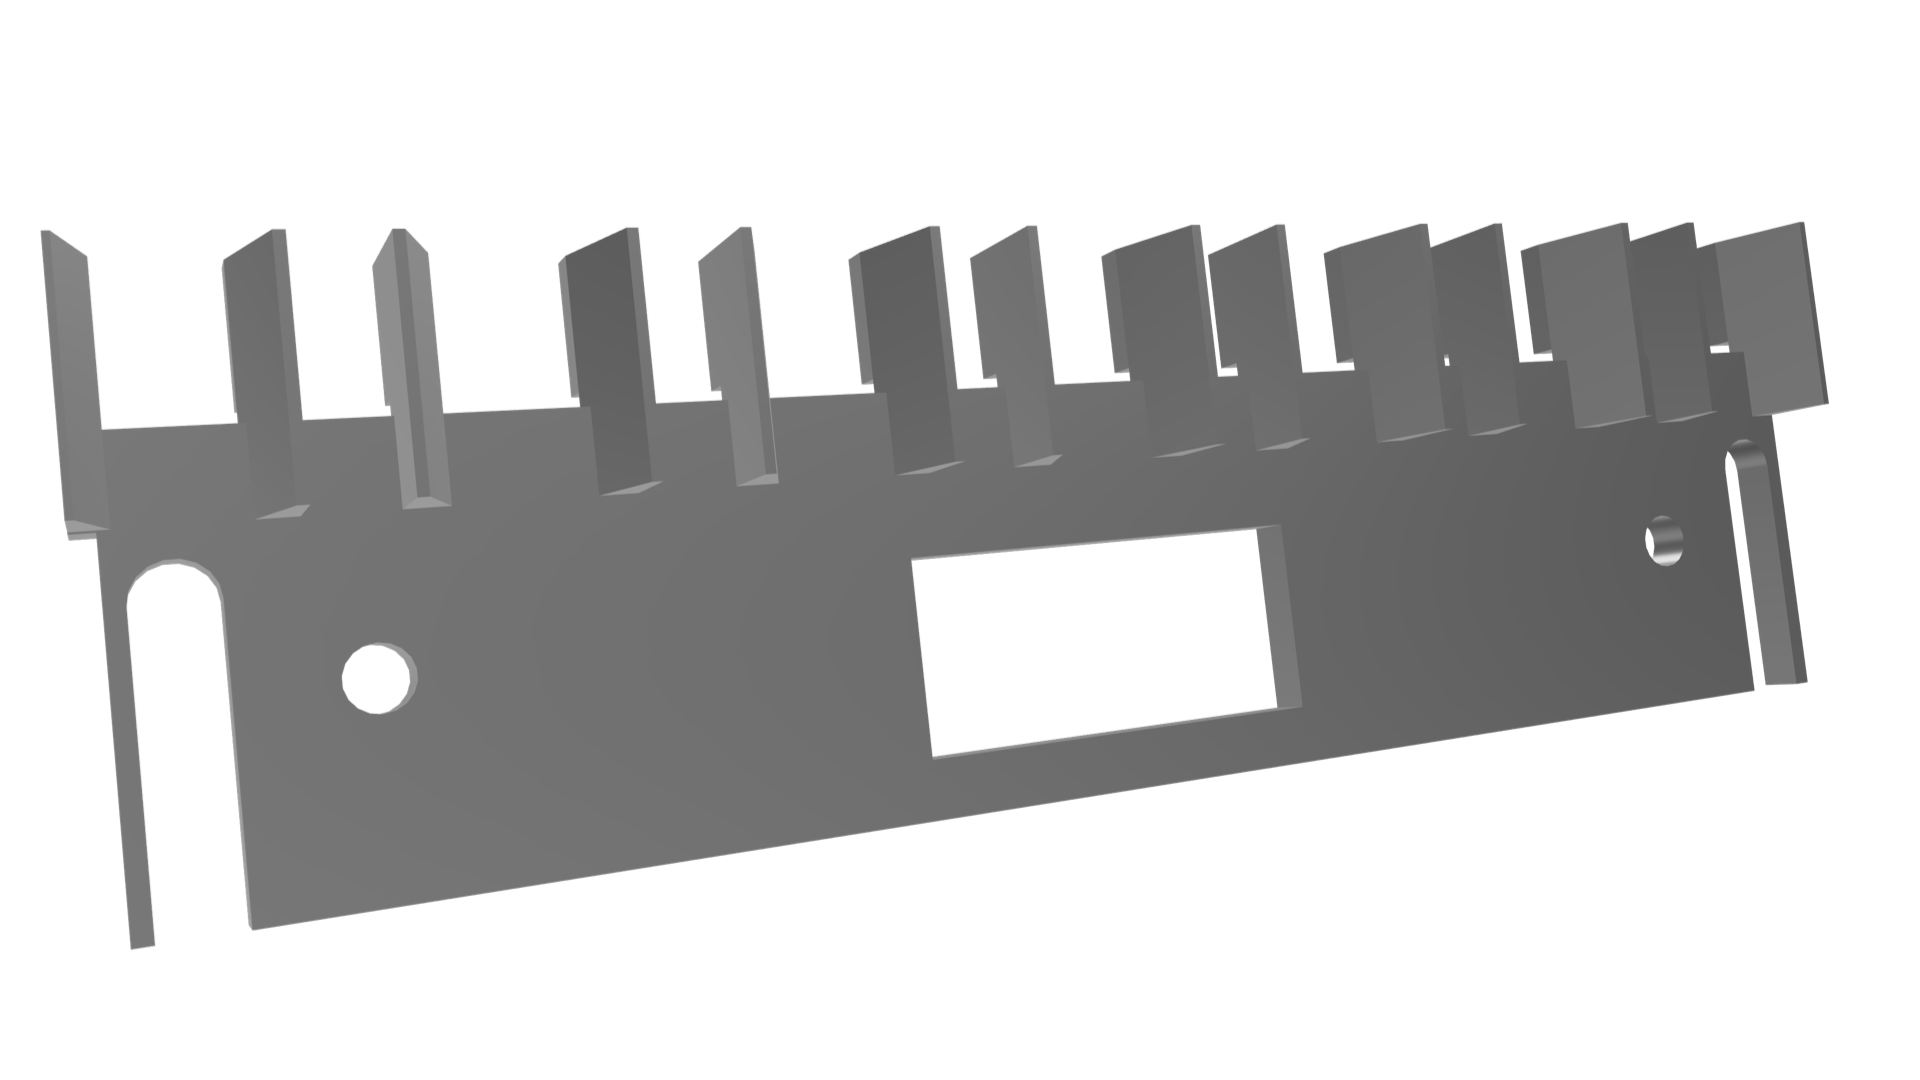
\includegraphics[width=0.8\linewidth,trim={0 2cm 0 2.5cm},clip]{img/baffles.png}
    \caption{Baffles designed to prevent cross-talk between adjacent sensors.}
    \label{fig:baffles}
\end{figure}

\begin{figure}
    \centering    
    \label{fig:sensor-bracket}
\end{figure}

\subsubsection{Controller Board}

\begin{figure}
    \centering
    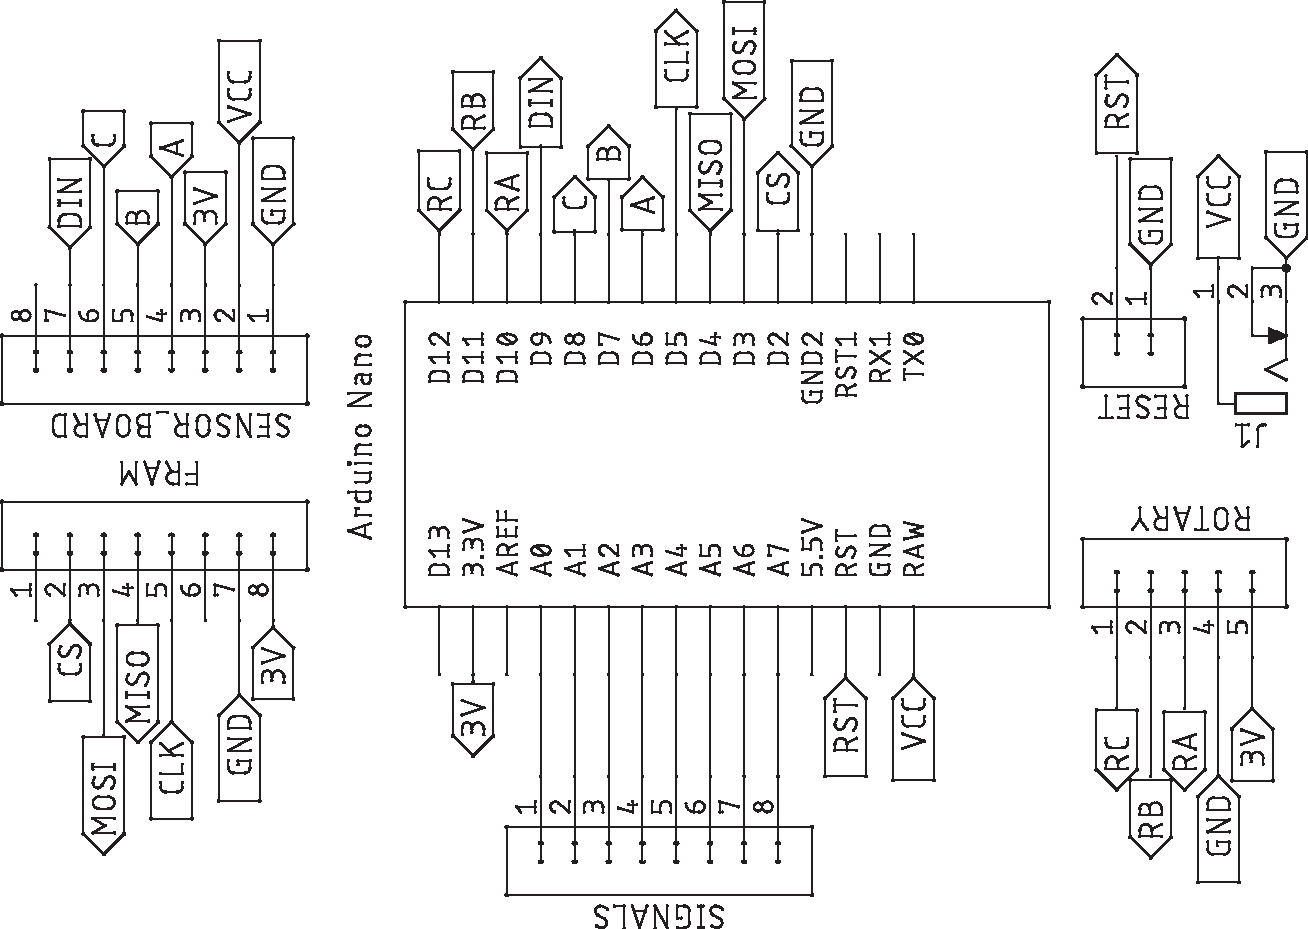
\includegraphics[width=0.75\linewidth,angle=180]{img/pcb_controller_schematic_v1.pdf}
    \caption{Mark 1 controller board schematic.}
    \label{fig:controller-schematic-1}
\end{figure}

The controller board was designed as means to reliably connect all components to the Nano BLE.
Figure~\ref{fig:controller-schematic-1} shows the schematic of the controller which illustrates its purpose to facilitate signal routing.  Components on the board are:

\begin{itemize}
    \item 1 Arduino Nano 33 BLE.
    \item 1 Fujitsu MB85RS64 SPI Ferroelectric RAM chip.
    \item 1 EC11 combined rotary encoder and tactile switch.
    \item 1 Momentary Reset Switch
\end{itemize}

Power is supplied through barrel jack \texttt{J1} and there are separate header connectors for the \texttt{RESET}, \texttt{ROTARY}, and \texttt{FRAM}. The connections to sensor board are separated into \texttt{SIGNALS} for the optical sensor signals and \texttt{SENSOR\_BOARD} containing the power, multiplexer channel select and LED control data. On the silkscreen of the final PCB (Figure~\ref{fig:controller-board-1}) the \texttt{SENSOR\_BOARD} header is marked as \texttt{FACEBOARD}


The Nano BLE is mounted to the PCB via header sockets. The header mount allowed for a second new Nano BLE to be quickly substituted should the original require a firmware update or become faulty. The firmware could not be update remotely and neither was there a reliable internet connection in the museum to do so. Ability to quick swap the Nano BLE aimed to avoid prolonged disruption to the exhibition. 

\begin{figure}
    \centering
    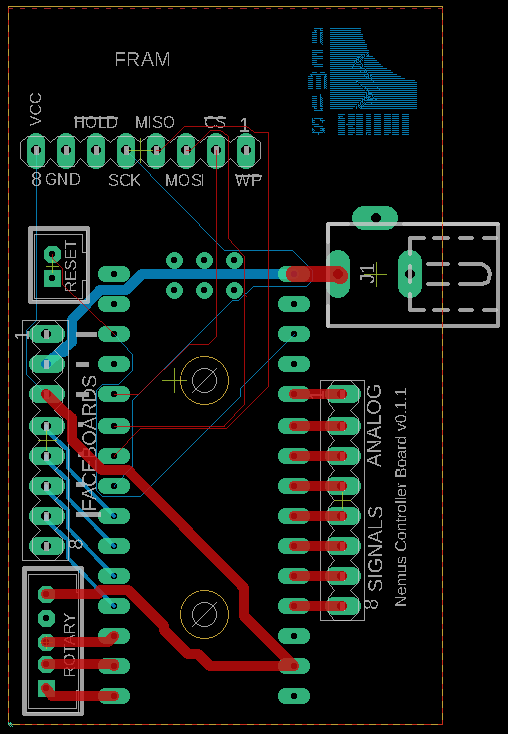
\includegraphics[angle=-90,width=0.66\linewidth]{img/pcb-controller-board-v0.1.0.png}
    \caption{Mark 1 controller board.}
    \label{fig:controller-board-1}
\end{figure}

The rotary encoder is used as an interface to the firmware and its functionality will be cobvered further in Section \ref{}. The reset switch is a simple momentary tactile switch that is installed toward the front of internal chamber. The rotary encoder and reset switches are attached to the con using a ribbon cable terminating in crimped 2.54-inch pitch connectors. 
The Nano BLE already has a reset switch attached to it, its position inside the Mark 1 made it difficult to reach. A reset could be performed with a power cycle, but this was neither practical nor ideal. Instead the reset switch gives the user more definite means of resetting the Nano BLE's firmware back to startup.

The power requirements for the system were estimated at 1.1 A at 5 V, with some
fluctuation when the system was first powered on. While the sensors were powered
continuously in this iteration, future designs may incorporate power-saving
measures, such as dynamic modulation of the optical emitters found \textcite{mcpherson_portable_2013}.

\subsection{Electronics Firmware}

The firmware begins by configuring the general purpose input and output (GPIO) pins and checking the FRAM is present after which it initiated in on of two states: a `calibration' and an `operation' state. The state is dictated by the whether the tactile switch of the rotary encoder is pressed as the firmware initiates. In the operation state, the optical sensors are read in sets of seven after which the multiplexer channel is incremented. The multiplexer channel is controlled through three GPIO pins labelled \texttt{A},\texttt{B} and \texttt{C} which combine as a 3-bit binary encoding (Table~\ref{tab:mux-encoding}).

\begin{table}[]
    \centering
    {
        \ttfamily
        \begin{tabular}{|c|c|c|c|}
            \hline
            C & B & A & MUX \\ \hline
            0 & 0 & 0 & 0   \\ \hline
            0 & 0 & 1 & 1   \\ \hline
            0 & 1 & 0 & 2   \\ \hline
            0 & 1 & 1 & 3   \\ \hline
            1 & 0 & 0 & 4   \\ \hline
            1 & 0 & 1 & 5   \\ \hline
            1 & 1 & 0 & 6   \\ \hline
            1 & 1 & 1 & 7   \\ \hline
        \end{tabular}
    }
    \caption{3-bit binary encoding for \texttt{MUX} channel selection. There are 8 \texttt{MUX} channels, indexed from 0.}
    \label{tab:mux-encoding}
\end{table}



A two-threshold hysteresis mechanism is used to implement a finite state machine with three states: \texttt{RELEASED}, \texttt{PLUCKED}, and \texttt{PRESSED}. 
A MIDI \texttt{Note\_ON} is triggered only when the sensor reading exceeds the \texttt{pluck\_threshold} and the system is in the \texttt{RELEASED} state. Conversely, a \texttt{Note\_OFF} is issued when the value falls below a lower \texttt{release\_threshold}, and the system is in the \texttt{PLUCKED} state (Figure~\ref{fig:jack-states}). This avoids instability from minor fluctuations near a single threshold and prevents rapid state toggling. A 4-sample moving average filter is applied to the sensor data to reduce high-frequency noise in the signal. The rise time of the sensors in combination with the averaging filter brought the effective sampling period to approximately 2 milliseconds with 1 millisecond jitter. The Nano BLE can be programmed with a interrupt function that can be set to a specific sample rate, however this was found to conflict with the monitoring required over the serial bus. Instead, the relative sampling period was measure by timing each iterations of the entire sensor read and processing cycle. The internal clock of the Nano BLE was polled at the start and end of each cycle and the time difference was stored in a buffer.  After ten-thousand cycles, the timing buffer was output over serial bus and a mean average of 1.7 milliseconds was found with a jitter of ±0.2 milliseconds, with both values rounded up to the nearest millisecond.

\begin{figure}
    \centering
    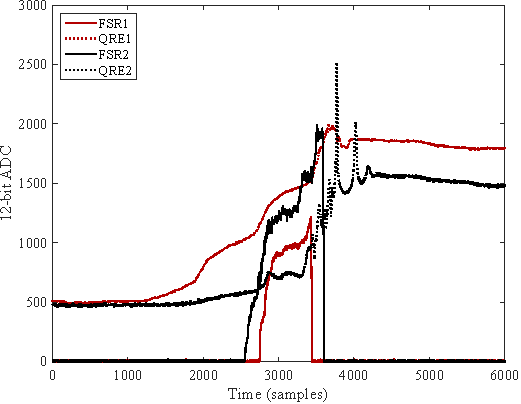
\includegraphics[width=0.66\linewidth]{img/plot-jack-states.pdf}
    \caption{Plot illustrating hysteresis as two thresholds. Plot shows a full key press and release event recorded using an Arduino Nano 33 BLE in its 12-bit DAC mode. After passing the pluck threshold, the key enters a \texttt{PLUCKED} state. The key then enters the \texttt{RELEASED} state after passing the lower release threshold.}
    \label{fig:jack-states}
\end{figure}


The thresholds for hysteresis are read from the connected FRAM module.
The data structure used for the thresholds was in part inspired by the RIFF file format standard \cite{ibm_riff_1991}. The layout of data was in such a way as to potentially allow for calibration values to be stored to files and read from either storage device or a binary on a file system. Table~\ref{tab:fram-structure} shows the structure of data in the FRAM. The pluck and release `Chunk IDs' can be interpreted as a unsigned 32-bit integer, with the hexadecimal values \texttt{0x4D415849} and \texttt{0x4D494E49} respectively or as ASCII character strings \texttt{"MAXI"} and \texttt{"MINI"}. The firmware checks memory addresses \texttt{0x00} and \texttt{0x66} for the corresponding Chunk ID and if the value stored there is not correct, the memory is  assumed to be uninitialised. In that case, the tag value is written and a default value will be set for all thresholds in the chunk.
A set wrapper functions was written for the FRAM library \footnote{Adafruit SPI FRAM Driver at version 2.6.2 \url{https://github.com/adafruit/Adafruit_FRAM_SPI/releases/tag/2.6.2}}. Doing so allowed the memory type used for reading threshold values to be more easily changed for another method, such as through an SD card.

\begin{table}
    \centering
    \begin{tabular}{|l|l|r|l|}
        \hline
        \textbf{Address} & \textbf{Field Name}     & \textbf{Size} & \textbf{C Type}        \\ \hline
        \texttt{0x00}    & Pluck Chunk ID          & 4             & \texttt{uint32\_t    } \\ \hline
        \texttt{0x04}    & Pluck Threshold Chunk   & 98            & \texttt{uint16\_t[49]} \\ \hline
        \texttt{0x66}    & Release Chunk ID        & 4             & \texttt{uint32\_t    } \\ \hline
        \texttt{0x6A}    & Release Threshold Chunk & 98            & \texttt{uint16\_t[49]} \\ \hline  
    \end{tabular}
    \caption{Calibration data layout in non-volatile memory.}
    \label{tab:fram-structure}
\end{table}

If the firmware starts in the `calibration state', the threshold values can modified and written to FRAM. In this mode, data from a single, selected sensor is written over the serial bus which can then be visualised. Figure~\ref{fig:serial_monitor} shows the threshold values being plotted , utilising the serial plotter of the Arduino IDE, alongside a live sensor reading to help identify the correct pluck point. The thresholds were calibrated first roughly calibrated in the NEM US laboratory through visual reference to the serial monitor (Figure \ref{fig:serial_monitor}) and the open source MIDI Monitor
software \footnote{\url{https://github.com/krevis/MIDIApps}}. The calibration workflow was carried out with the support of Dr. Craig Webb who, being unfamiliar with the system, could help with drawing up a workflow to disseminate to an untrained user. Adjustments were made to the firmware to to make it more intuitive for the staff at San Colombano where a finer calibration process was carried out with the guidance of expert harpsichord performer Catalina Vicens.
A MIDI message is generated as the sensor reading passes the thresholds allowing the user to audition the keyboard with a sampler and adjust the thresholds accordingly. The jack's corresponding LED reports with colours green (\texttt{PLUCKED}), orange (\texttt{PRESSED}) and blue (\texttt{RELEASED}) for quick visual confirmation of key state. Red is used to indicate sensor readings outside expected values that are close to either the minimum or maximum of the ADC, which would indicate a malfunctioning or misaligned sensor board.

\begin{figure}  
  \centering
  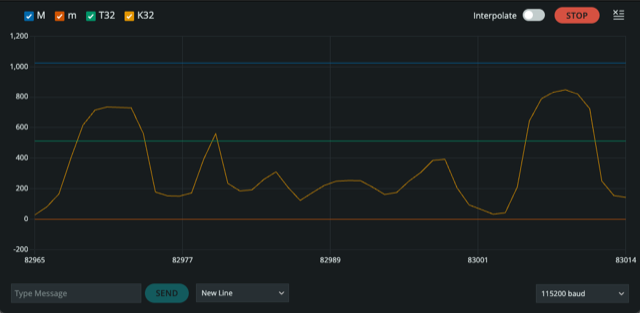
\includegraphics[width=1\linewidth]{img/serial_monitor.png} 
  \caption{Example of calibrating a pluck threshold using the Arduino IDE Serial Plotter in a 10-bit ADC mode. Plot shows the key at index 32 (\texttt{K32}) and its current pluck threshold (\texttt{T32}). \texttt{M} and \texttt{m} are the maximum and minimum values to normalise the y axis of the plot.}   
  \label{fig:serial_monitor}
\end{figure}

\subsection{Installation}

\begin{figure}
    \centering
    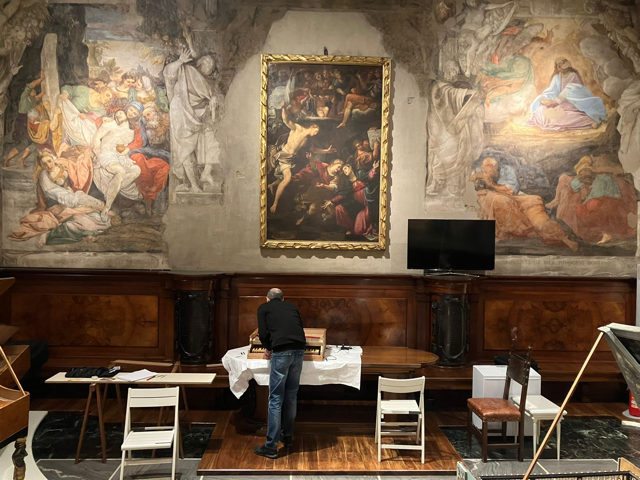
\includegraphics[width=0.5\linewidth]{img/installation.png}
    \caption{Keyboard being installed for exhibition in the Oratory at San Colombano.}
    \label{fig:installation}
\end{figure}

Once a sensor system had been fabricated, the next stage was to install it within the mechanical interface.  Electronics were designed to be a bespoke installation, after which brackets and enclosures could be drafted to hasten the install process. This also provided flexibility to adjust wiring and fitting should there be any unforeseen problems. One such problem was the change from a horizontal to a vertical design

The electronic components were partly pre-assembled at the university of
Edinburgh. Though all measurements were known ahead, enough flexibility was
needed to allow for problems to be solved in situ.

The final assembly took place at the NEMUS lab at the University of Bologna over
the final week in October 2024 for delivery at San Colombano for exhibition in
the first week of November 2024.

The PCBs shared power and data lines for components with the exception of the
output from the multiplexer. Ribbon cable was cut to size to allow for some room
to readjust the distance of the sensors from the jacks. The data signals from
each PCB were connected using a separate cable loom. Soldering cables and
inspecting each join required another day work. This did allow for readjustments
to the position of the controller board Measurements of the rear chamber did not
match with the Mac Mini that was to be used a different layout was decided for
fitting the controller board/ Cutting cables to size allowed for a great deal of
flexibility but at the cost of time. After the first install it was clearer what
constraints were in place for fitting and an alternative wiring system using
flat flex cable was implement (discussed in \textbackslash section)

Fitting PCBs required the removal of all keys. The support brackets were
assembled and screwed into the the underside. With the harpsichord on it's back
the sensors were tested to ensure an expected range. Self-tapping round head
screws were used to to attach the brackets. The screws were not over tightened
to allow for brackets to move. The brackets were not easily adjusted once the
key were replaced. Adjusted to a best average with subsequent adjustment carried
out on the microcontroller.

As the PCBs were fitted the jacks had the gradient stickers applied to them. The
jacks had been coated with a varnish on the short side to provide a better
surface for the stickers to adhere to. After the stickers were applied excess
material was trimmed from each jack. The jack were then check that they moved
freely in their slot.

After fitting the PCBs, preliminary calibration was carried out. Before the keys
were refitted, the jacks were put back in position. The data from each jack was
confirmed to be in a expected range. Any jack that showed anomalous data was removed and re-inspected. The fitting and refitting of sensor system required another
day as faults were found in wiring or misalignment of the gradient stickers. After the
sensors were confirmed to be functioning the keys were put back.

A typo in the original clearance between the keys and the sensor board resulted in the 
the keys being blocked entirely from moving. A 10 mm by 15 mm section was milled
out of each key to create extra clearance (Figure~\ref{fig:milling)}. The milling required the removal, shortening and refitting of the leather pads for the jacks. The extra work added
an extra day to the full install.

\begin{figure}  
  \centering
  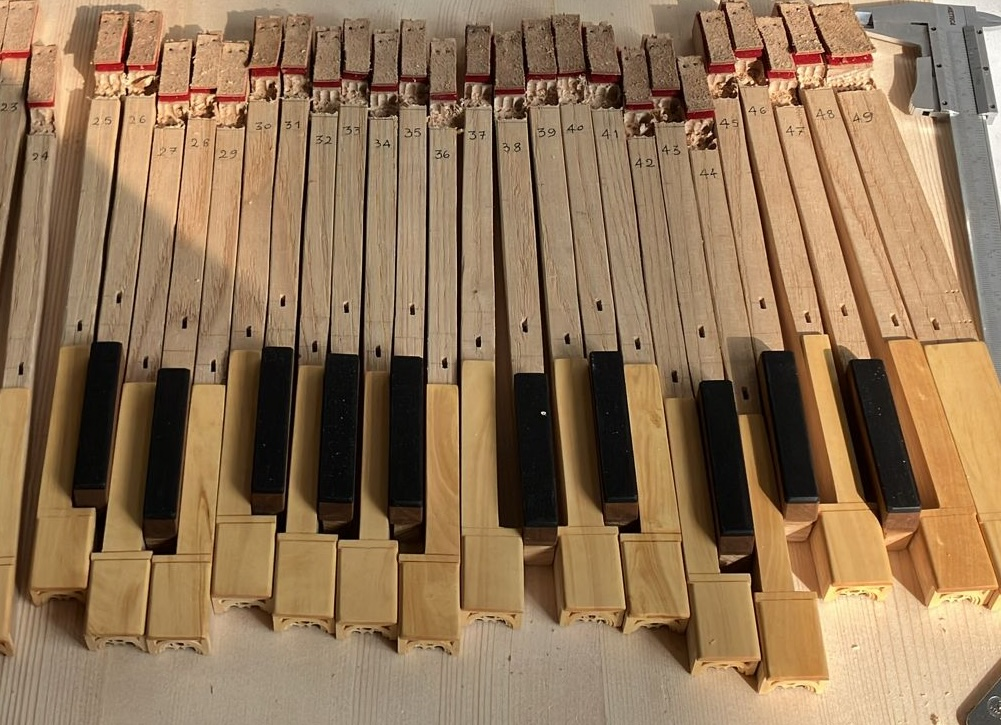
\includegraphics[width=0.75\linewidth]{img/keys-milled.jpeg}\\
  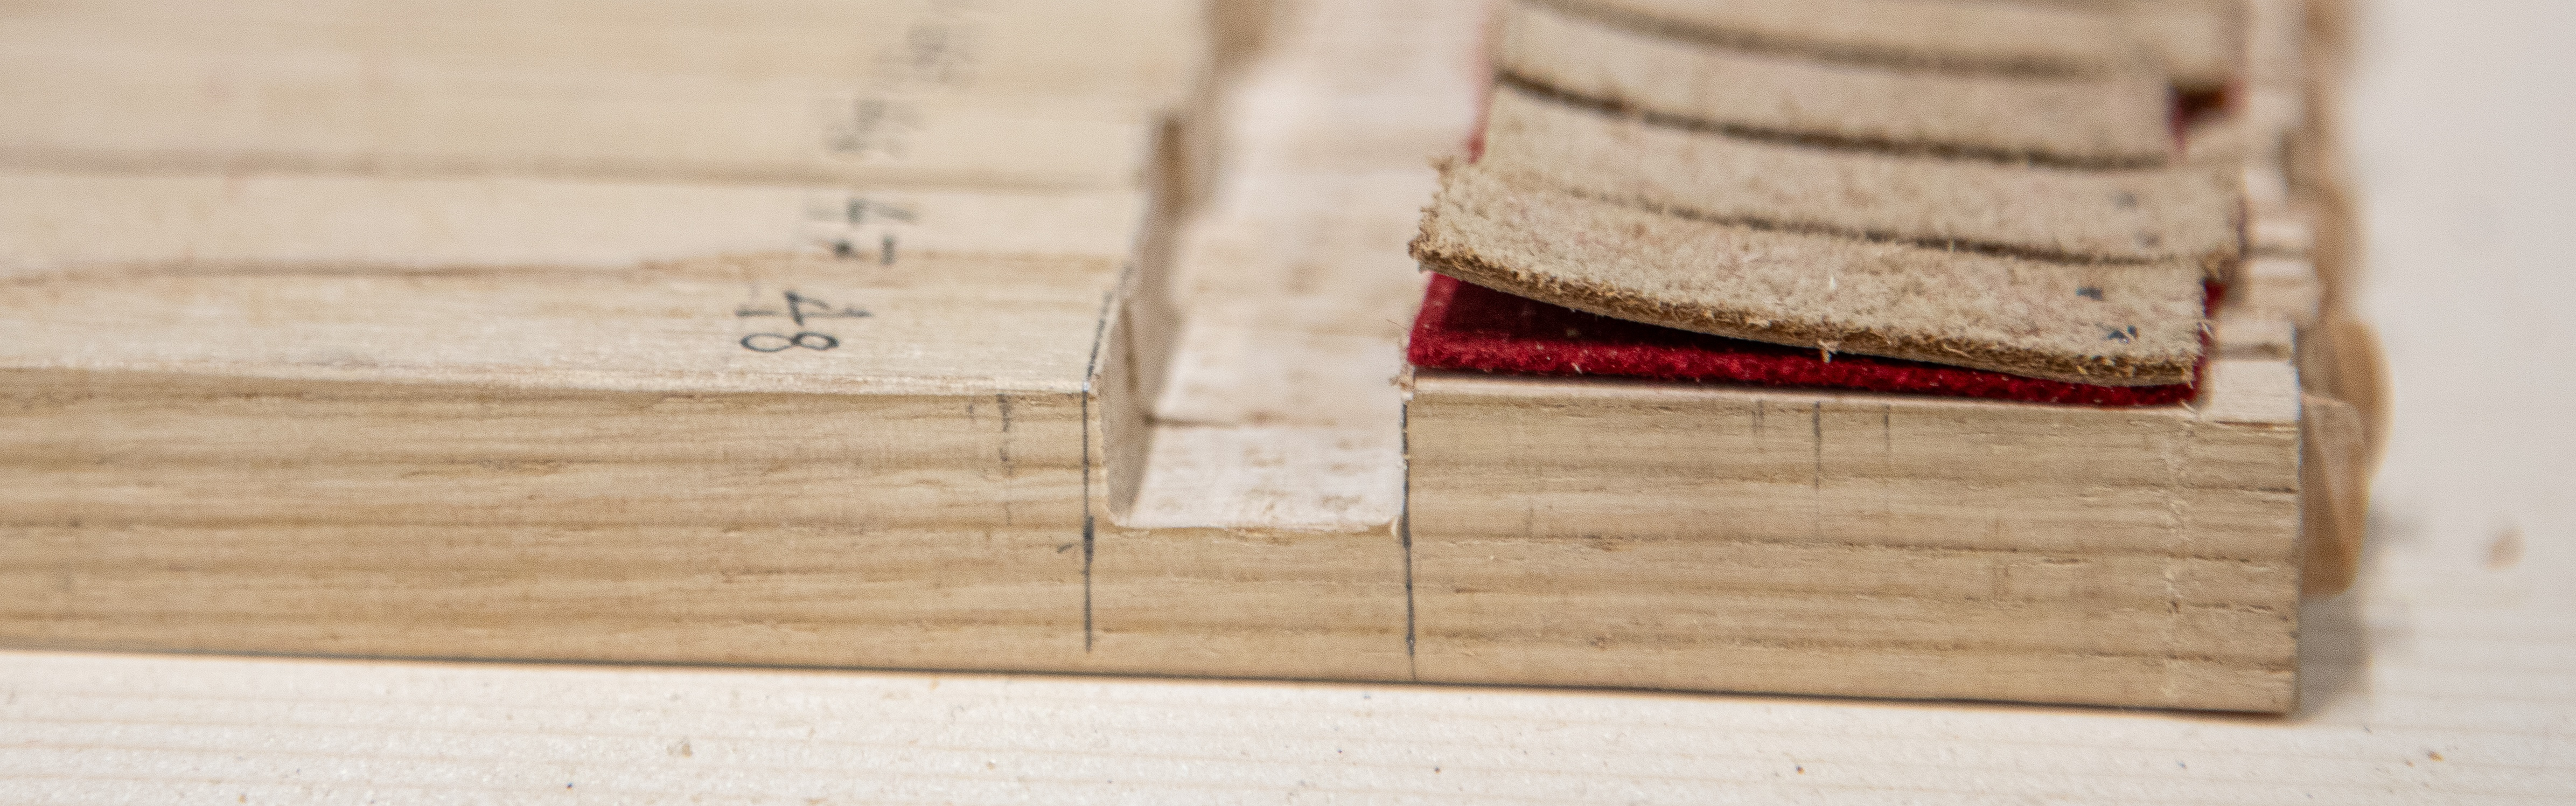
\includegraphics[width=0.75\linewidth]{img/milled-keys.jpg} 
  \caption{Keys after rough milling (Top) and after squaring and finishing the new cavity (Bottom).} 
  \label{fig:milling}
\end{figure}

The later redesign of the PCBs for the Mark 2 interface meant that removing the material would not b e necessary.

For the initial version of the exhibition, a harpsichord sample library was used
and controlled via Native Instrument's
Kontakt\footnote{\href{https://www.native-instruments.com/en/products/komplete/samplers/kontakt-8/?srsltid=AfmBOorKUf43SoIxGBS2-GnXmKHHkgcfcfWRskpweDhLSG3FiF0qrf2w}{Kontakt
webpage} (Accessed 31 Jan 2025)}. The software was installed on a Mac Mini
hosted inside the instrument's case. Holes were drilled at the back of the
instrument's frame, away from sight, to allow the passage of cables, such as
from power supplies, USB connectors and headphone jack (Figure
\ref{fig:mac-mini}). An iPad is used as a monitor through which visitors can
adjust playback parameters such as tuning, voicing and which stops are engaged. 

\begin{figure}
    \centering
    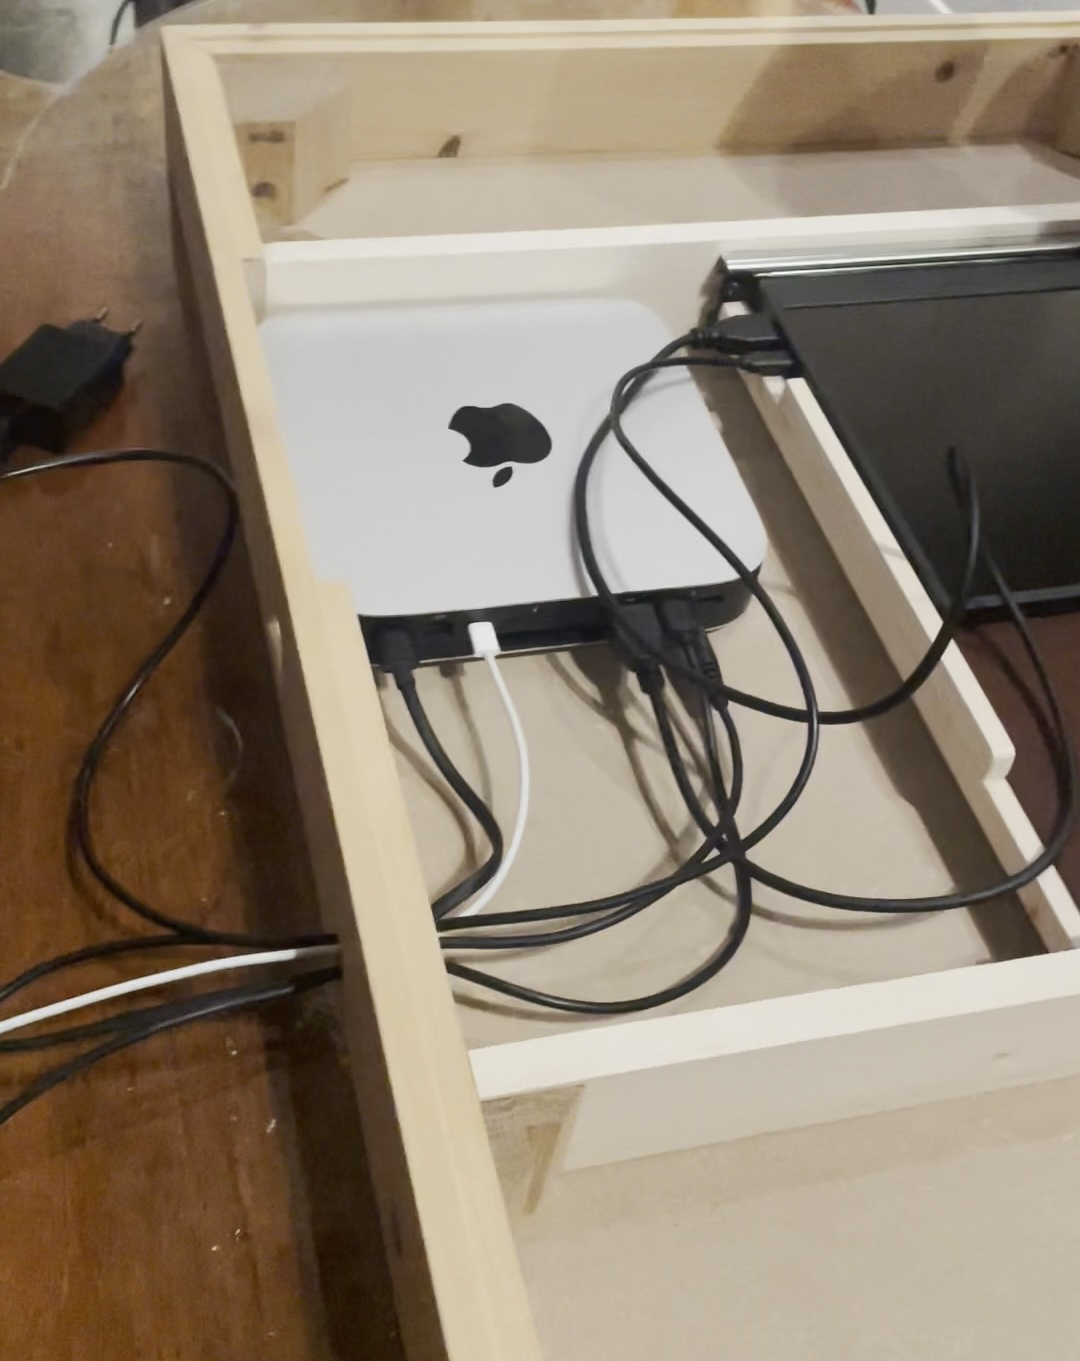
\includegraphics[width=0.8\linewidth,trim={0 5cm 0 0},clip]{img/mac-mini.jpg}
    \caption{Components and cabling hidden in the bottom section of the instrument case.}
    \label{fig:mac-mini}
\end{figure}

\subsection{Calibration}

Used as the interface to select a key, edit a threshold and
save current thresholds to the FRAM. Thresholds were first set the midrange of
possible values a a default. A rough calibration process was carried out where
each sensor were selected individually and its readings were plotted against
their current threshold value using the Arduino IDE serial plotter. Thresholds
were adjusted with the rotary encoder until the key no longer passed the
threshold line until the jack had plucked the string. During calibration RGB
LEDs were used as a visual aid to quickly identify which key was currently being
adjusted. These LEDs also provided visual feedback during calibration, and would
change colour based on if readings were above below the threshold or if the were
outside previously recorded maximum or minimum values. Such use of the LEDs
meant for easy identification of malfunctioning sensors and simplified the
alignment process. 

\subsection{Open Sourcing}

The open source repository encompassed all aspects of the system.
Following best practice in the DMI community \cite{calegario_documentation_2021}, and broader academia \cite{stall_journal_2023}, the digital assets for the interface were placed under version control and archived. These assets included,

\begin{multicols}{2}
\begin{itemize}
  \item Source Code
  \item Textual Description(s)
  \item Bill of Materials
  \item Build and Operational Instructions
  \item Photo(s) / Image(s) / Diagram(s) / Drawing(s)
  \item STL model files
  \item CAD PCB Schematice files
\end{itemize}
\end{multicols}

All of these digital assets were divided into one of three version control repositories: \emph{Firmware}, \emph{CAD}, and \emph{Model data}. The firmware repository \cite{hamilton_firmware_2025} contains all source code for final firmware, test firmware and documentation of usage and dependencies. The CAD repository \cite{hamilton_cad_2025} EAGLE CAD contains files and bill of materials for electronics. Finally, the Models repository \cite{hamilton_models_2025} contains the STL 3D models for the jacks and physical measurement for the mechanical interface. These repositories are combined into a single meta repository (Figure~\ref{fig:repo-relation}) as `sub-module' a reference to a git repository as it existed for a specific moment in time. Each sub-module can be considered in isolation and reused as a component of another project.  It is only when they are combined in \textcite{hamilton_nemus_2025} that they represent the interface as it was deployed at Museo San Colombano. This allows for substitutions in any repository should there be a changes such as the type of optical sensor used or the type mechanical hardware used. Sub-modules also promote a containerised methodology, where any component (i.e. sub-module) can be developed without affecting the larger meta-repository. Updating any one sub-module is therefore a conscious decision and not an accidental or unavoidable by product of changing the constituent parts. 

\begin{figure}
\centering
    \begin{tikzpicture}[
      box/.style = {draw, minimum width=3cm, minimum height=1.5cm, align=center},
      arrow/.style = {-latex', thick}
    ]
    
    % Top boxes
    \node[box] (box1) {Firmware\\sub-module};
    \node[box, right=of box1] (box2) {CAD\\sub-module};
    \node[box, right=of box2] (box3) {Model Data\\sub-module};
    
    % Bottom box
    \node[box, below=2cm of box2] (bottom) {Interface\\meta-repository};
    
    % Arrows from bottom box to each top box
    \draw[arrow] (bottom.north) -- (box1.south);
    \draw[arrow] (bottom.north) -- (box2.south);
    \draw[arrow] (bottom.north) -- (box3.south);
    
    \end{tikzpicture}

    \caption{Interface git repository and its submodules}
    \label{fig:repo-relation}
\end{figure}

Though a sub-module approach to the project was beneficial during development, organisation in this manner highlighted limitations the archiving process. A major benefit of the Zenodo archiving platform is its integration to GitHub. This allows a single project to be simultaneously maintained and archived for citation from a single location.
Unfortunately, the GitHub integration for Zenodo does not currently provide a means for meta-repositories to be archived correctly \cite{zenodo_1036_2025}. This limitation necessitates the generation of a separate DOI for each component submodule, all of which reference the meta-repository.

CAD files and surrounding support files also provide another point of failure with respect to digital preservation. For example, in the course of this thesis the popular Electronic Design Automation (EDA) software tool EAGLE was announced to be discontinued \cite{autodesk_eagle_2024} for the July 2026. A conscious decision was made to continue using the EAGLE format for the PCB design. Much in the same way as the discontinuation of Python 2 may be beneficial for archival purposes as ``advanced programming language that is guaranteed not to evolve anymore'' \cite{rougier_loupe_2020}, so to does the discontinuation of the EAGLE means that its XML file standard is now calcified and is unable changes. Instead, the EAGLE files can be used in conjunction with other EDA software such as the open source KiCAD \cite{kicad_eagle_2024}.

\section{Exhibition}\label{interfacing-with-digital-instrument}


The exhibition opened February 2025 and the Mark 1 is installed in the \emph{Oratory} at San Colombano alongside unique examples of the Italian Renaissance building tradition,
including the 1547 harpsichord and the 1540 spinet by Alessandro Trasuntino \footnote{https://digital.fondazionecarisbo.it/artwork/arpicordo-a-pianta-poligonale-anonimo-attr-ad-alessandro-trasuntino} from which the design was partly inspired.
Since the exhibition opening there have been two rounds of preliminary feedback collected. The first from a pool of 20 people -- consisting of staff, surveillance personnel and visitors who were given training on the system -- and expert feedback from curator Catalina Vicens and luthier Roberto Livi.The keyboard shows
promise in enhancing the museum experience as comments about a ``sense of
disconnect'' found in the Benton Fletcher Collection
\cite{mcalpine_sampling_2014} were absent in this initial feedback.


Expert feedback has highlighted limitations, including imprecise key
calibration, which creates a temporal disconnect between the tactile plucking
sensation and sound onset. Additionally, the commercial sample library, while
allowing the selection of registers such as 8', 4', and their combinations,
restricts functionality to a single MIDI message per key, regardless of the
number of string choirs controlled. Inspired by early Italian instruments, the
keyboard's layout is designed to manage two 8' registers with a sensor system
fitted to each. Internally, the instrument functions as two separate MIDI
devices. However, one register must be disengaged due to the software's limited
communication with only a single device. While running multiple instances of the
software is possible, having two sets of GUI controls was considered too
confusing for visitors engaging with the exhibition without prior orientation.
Consequently, sensors are only active on single jacks to accommodate these
constraints. Future iterations could address these limitations through technical
improvements, such as refined calibration with hysteresis and developing a
custom sample library and interface.

The second round as part of a wider survey of the exhibition on a group of approximately 50 PhD students. This survey was in a five-point scale format the results of which are still being collected. From this group it was observed that some did not play the interface. When these visitors were later asked why they did not play the reasons given were that did not think they were allowed to touch the instrument. This behaviour could be considered a compliment to the accuracy of the keyboard's aesthetics, but may also suggest a wider problem with encouraging interaction in the museum context.

% A more formal surveying of museum visitors would be required to determine to
% what degree the exhibition achieved its core aims. The keyboard is hosted in the
% \emph{Oratory} above the museum's main hall, an exceptional testimony to the
% Bolognese art, decorated by the finest students of the Carracci and presenting a
% series of frescoes covering most of the walls and ceiling. The room hosts unique
% examples of the Italian Renaissance building tradition, including the 1547
% harpsichord and the 1540 spinet by Alessandro Trasuntino. Visitors often
% visit the room with the same caution and respect typical of worship spaces.
% Among the visitors interviewed, no comments were made that the exposed
% headphones and touchscreen affected such an experience negatively, though a more
% definitive answer will come as more feedback is collected after launch. Pictures
% of the keyboard hosted in the \emph{Oratory} are shown in Figure
% \ref{fig:oratory}.

\begin{figure}
    \centering
    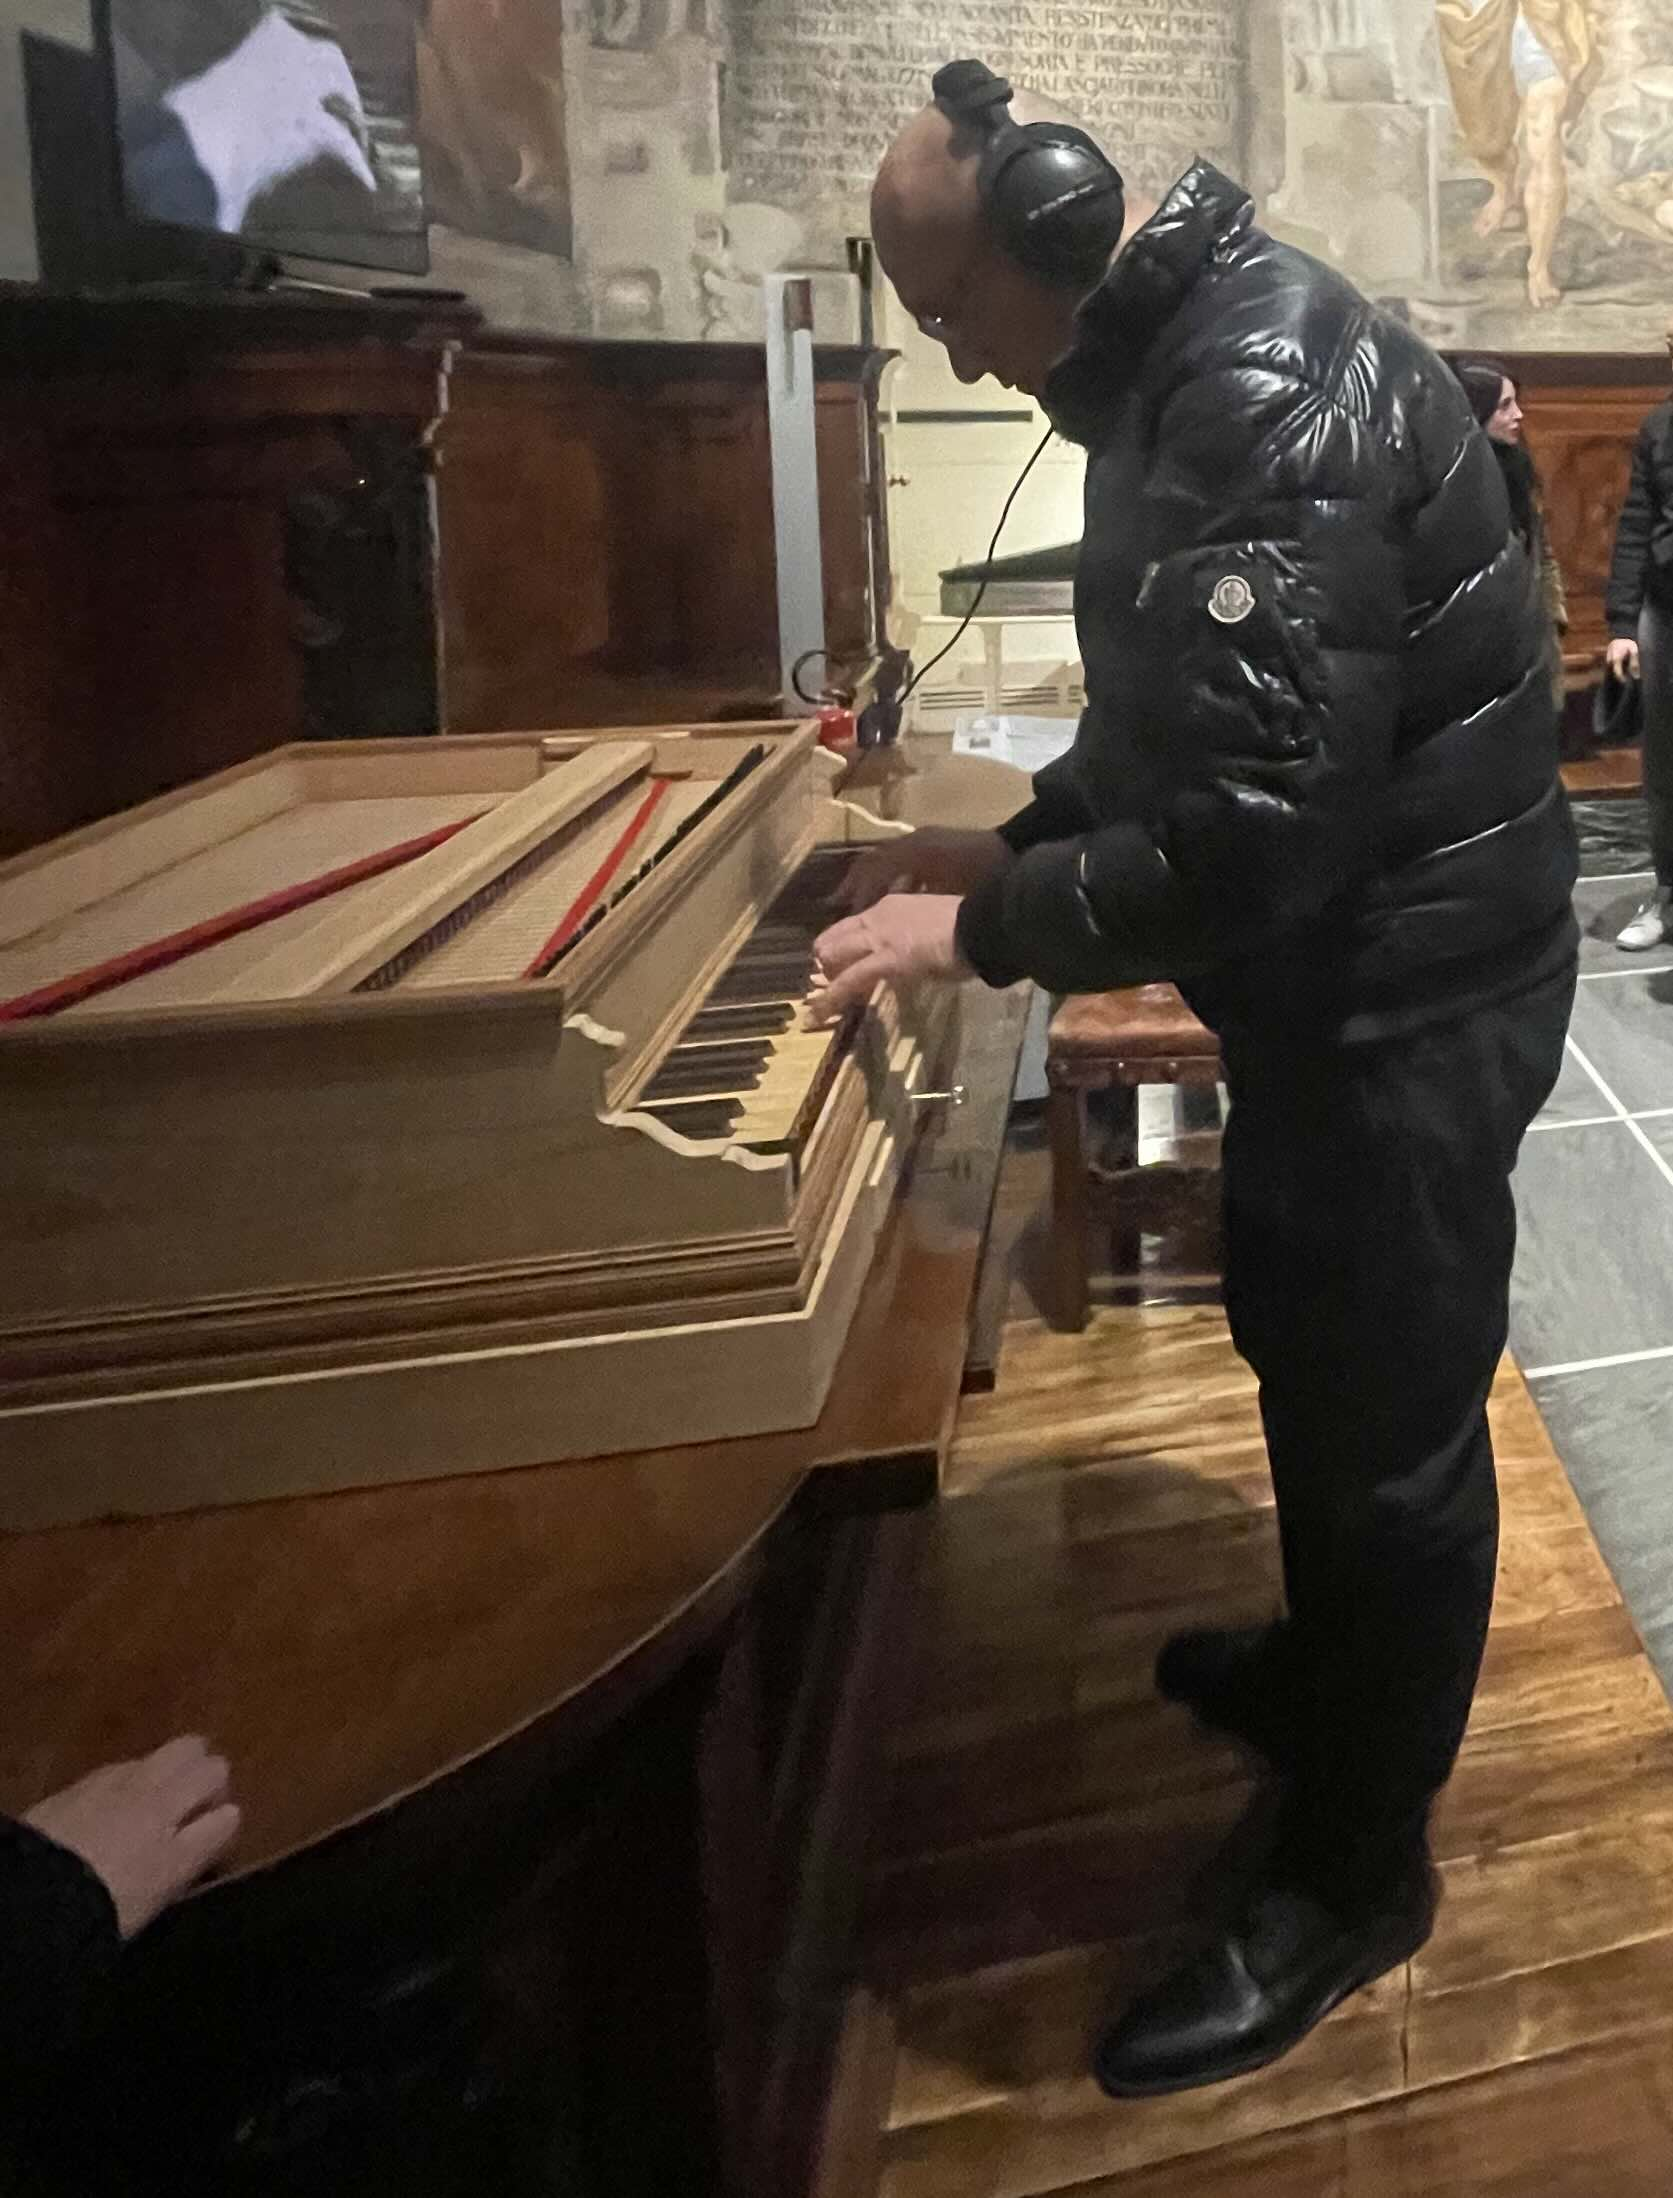
\includegraphics[height=0.5\linewidth]{img/exhibition-user-2.jpg}
    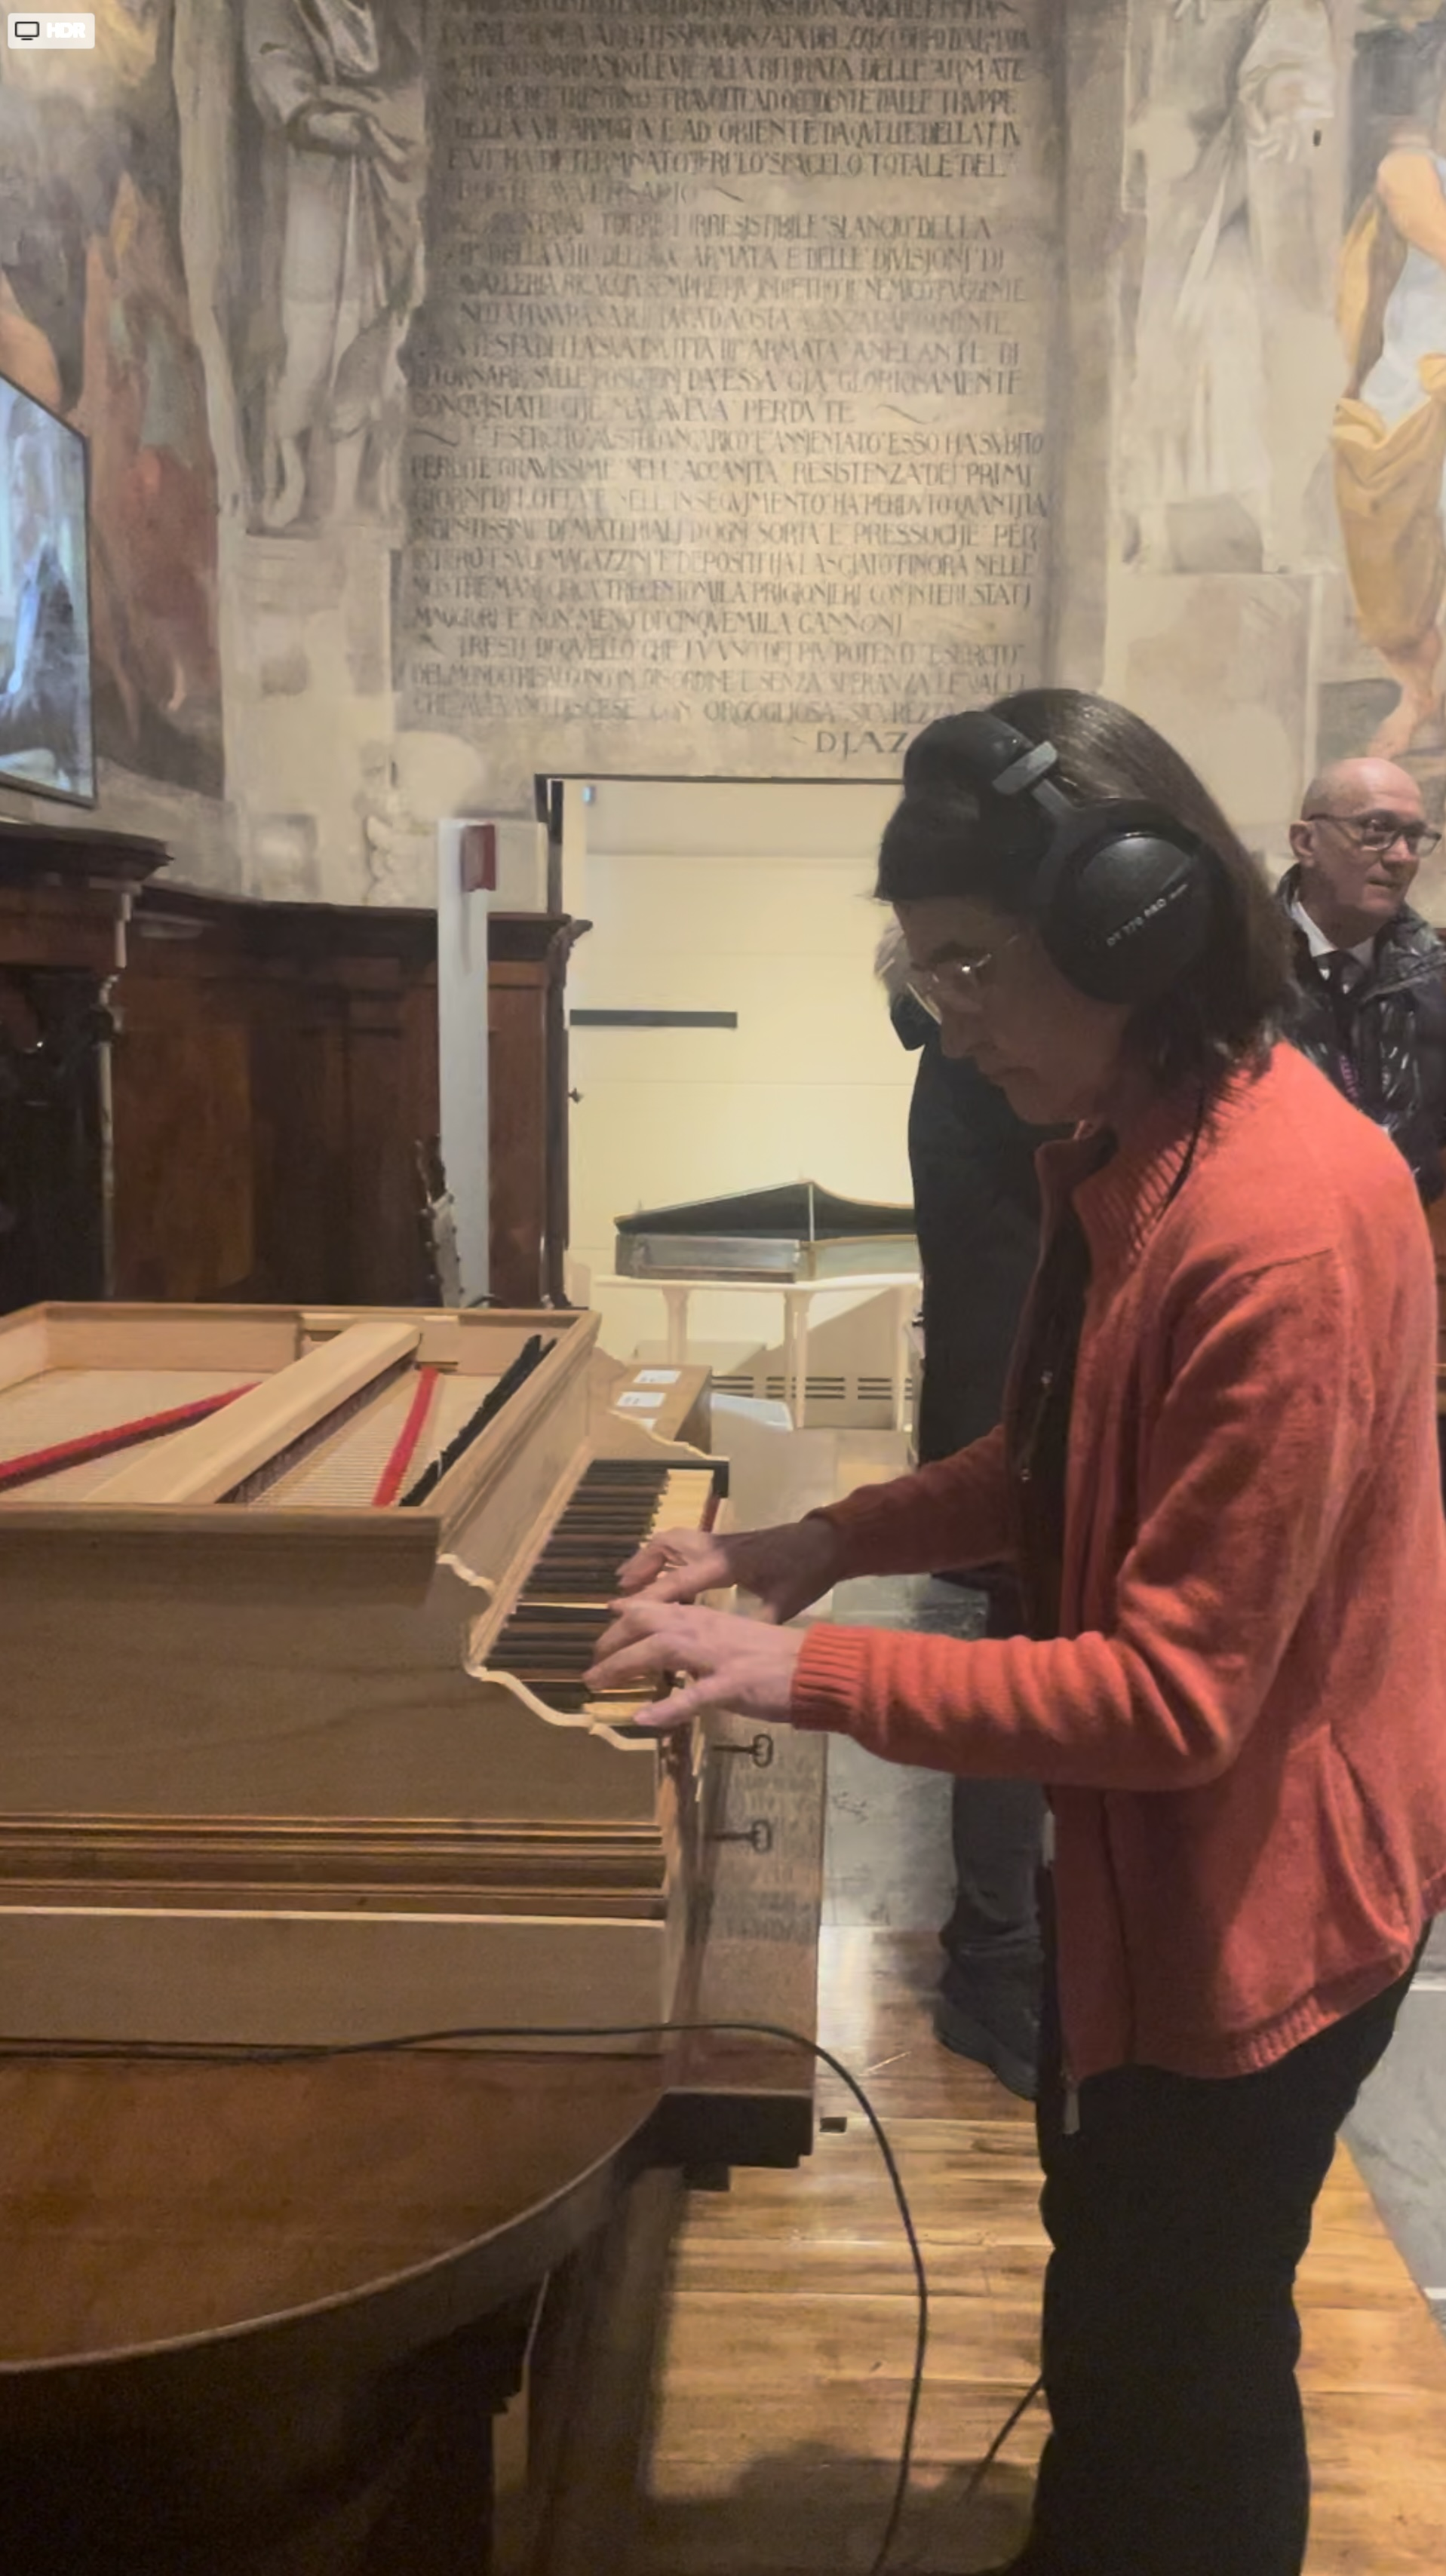
\includegraphics[height=0.5\linewidth]{img/exhibition-user-3.jpg}
    \caption{The keyboard installed in the \emph{Oratory} at San Colombano,
    and a user wearing headphones playing it.}
    \label{fig:oratory}
\end{figure}



\section{Mark 2}

\begin{figure}
    \centering
    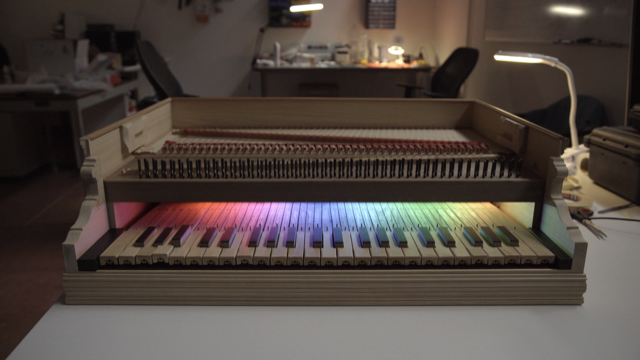
\includegraphics[width=0.7\linewidth]{img/mark2.png}\\
    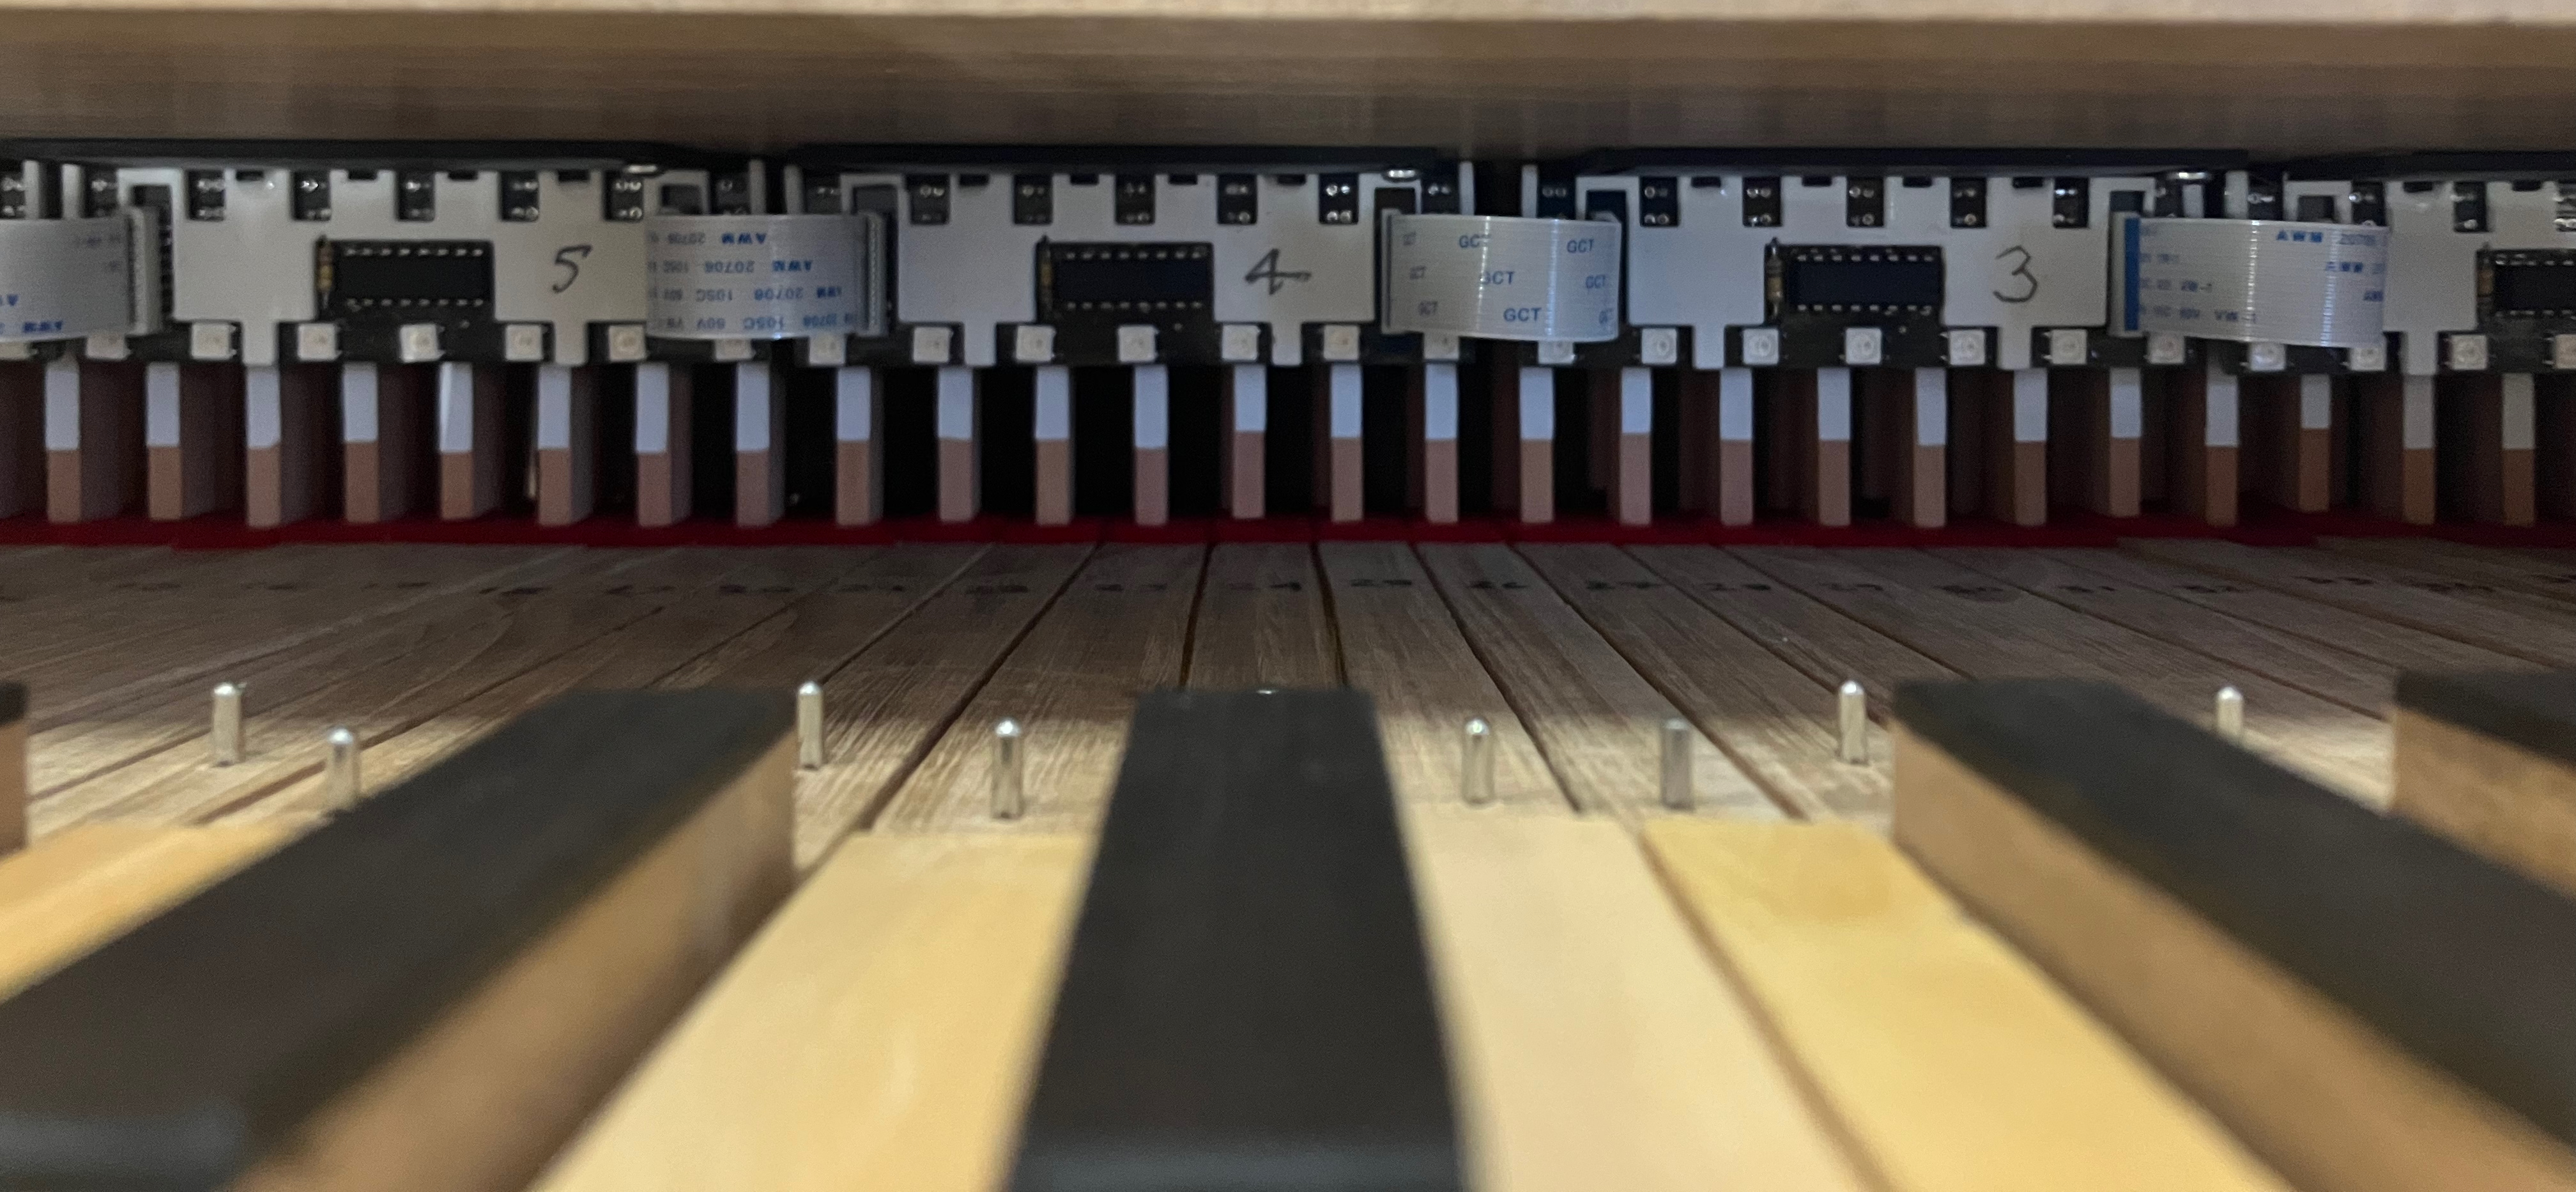
\includegraphics[width=0.7\linewidth,trim={0 20cm 0 .5cm},clip]{img/mark-2-front-internal.jpeg}
    \caption{Mark 2 [Image Credit] (Top) and the front register sensor boards behind the nameplate (Bottom)}
    \label{fig:mark-2}
\end{figure}

Using what had been learned in the design and deployment of the Mark 1 interface, a second interface was designed and commissioned again by NEMUS for fabrication by Roberto Livi. This interface, referred to a Mark 2, would be used as part of research in the NEMUS laboratory for interaction with an audio synthesis engine using numerical simulated physical models using the multiple register functionality of the interface. The Mark 2 demonstrates a refinement of the sensor technology and full functionality of a multiple register system. Python was used to create script files for the Eagle CAD software that allowed for parametric placement of components based on the pitch spacing of the jacks, expediting the design process.

The mechanical interface for Mark 2 differed from Mark 1 in that it was designed with 45 keys instead of 49, which was chosen to match the common short octave configuration found in historical Italian plucked keyboard instruments from the XVI to the XVIII century \cite[p. 46]{tagliavini_clavicembali_1987}. The short octave could then be mapped directly to MIDI notes within the firmware.

% \subsubsection{Developments}

% \begin{figure}
%   \centering
%   \begin{subfigure}[h]{0.5\linewidth}
%     \centering
%     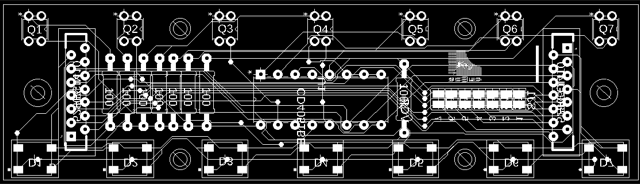
\includegraphics[height=0.2\linewidth]{img/pcb_sensor_board_v2.png}
%     \caption{Sensor PCB}
%     \label{fig:sensor_v2}
%   \end{subfigure}
%   \begin{subfigure}[h]{0.4\linewidth}
%     \centering
%     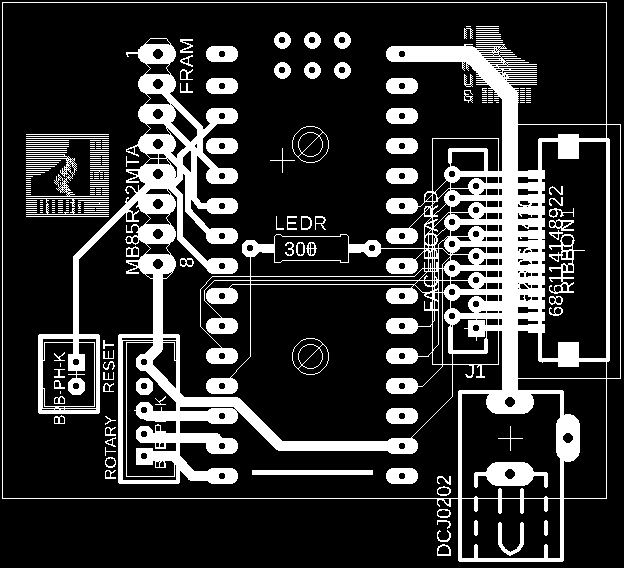
\includegraphics[height=0.2\linewidth]{img/pcb_controller_board_v2.png}
%     \caption{Controller PCB}
%     \label{fig:controller_v2}
%   \end{subfigure}
%   \caption{PCB traces of the redesigned sensor and controller boards. Figure show the inclusion of FFC and JST-PH ports. Sensor board shows the solder pads used to configure its position in the keyboard}
%   \label{fig:pcb_v2}
% \end{figure}

\begin{figure}
    \centering    
    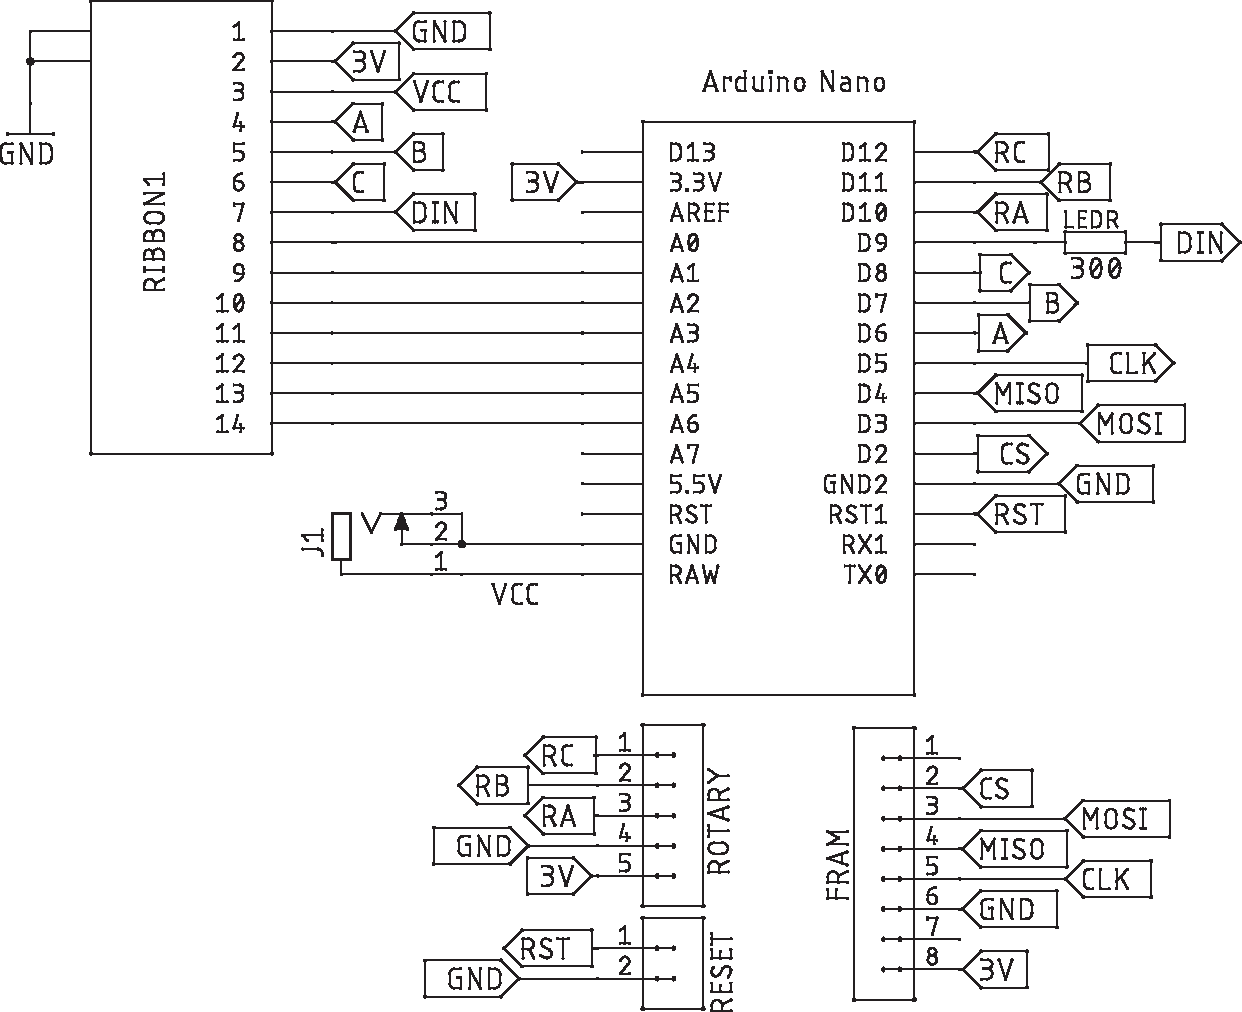
\includegraphics[width=0.5\linewidth]{img/pcb_controller_schematic_v2.pdf}
    \caption{Controller board schematic version 2.}
    \label{fig:controller-schematic-2}
\end{figure}

The redesign of the controller board (Figure~\ref{fig:controller-schematic-2}) added JST-PH ports for the FRAM, rotary encoder, and reset switch. The JST-PH connector has a locator which stops the cable from becoming disconnected easily.
Both the JST-PH and FFC ports are asymmetric which ensured only a single orientation of connection is possible and prevented incorrect wiring during installation. The FFC cables on the sensor PCB, visible in Figure~\ref{fig:mark-2}, permitted quick connection of the sensor boards and the flat form allowed the cabling the to be routed between the joins of the keyboard frame and the outer frame.

The original seven sensors per board was kept and the two sensor on the edges of the board are simply not used.  Reducing the number of sensors on the PCB would have meant increasing the number of PCBs required. This in turn would require more multiplexers which would have half of their channels unused. Keeping the sensor board format the same also mean the firmware could be reused with little modification.

\begin{figure}
    \centering
    \includesvg[inkscapelatex=false, width=0.8\linewidth]{img/pcb_sensor_schematic_v2.svg}    
    \caption{Mark 2 Sensor board schematic. RGB LEDs \texttt{D}, signal paths \texttt{S}, optical sensors \texttt{Q}. The Solder Junction in the center illustrates the connection  between the multiplexer output and corresponding \texttt{S} channel assignment on the FFC cable. Labels point in the direction of current flow.}
    \label{fig:sensor-schematic-2}
\end{figure}


A major change to the sensor board was the inclusion of a solder pad junction (Figure~\ref{fig:sensor-schematic-2}). The junction is a set of solder pads which can be shorted. This then set to which ADC channel on the Nano BLE the signal is routed. In combination with the FFC cable, this allowed a single board to be easily substituted should there be a fault with any components. For Mark 1, the wiring was such that any one board required disconnection of the entire system and access to soldering facilities. The FFC and solder junction provided a means to create a replacement off site from the museum and swap the faulty board in situ.

% \begin{figure}
%   \centering
%   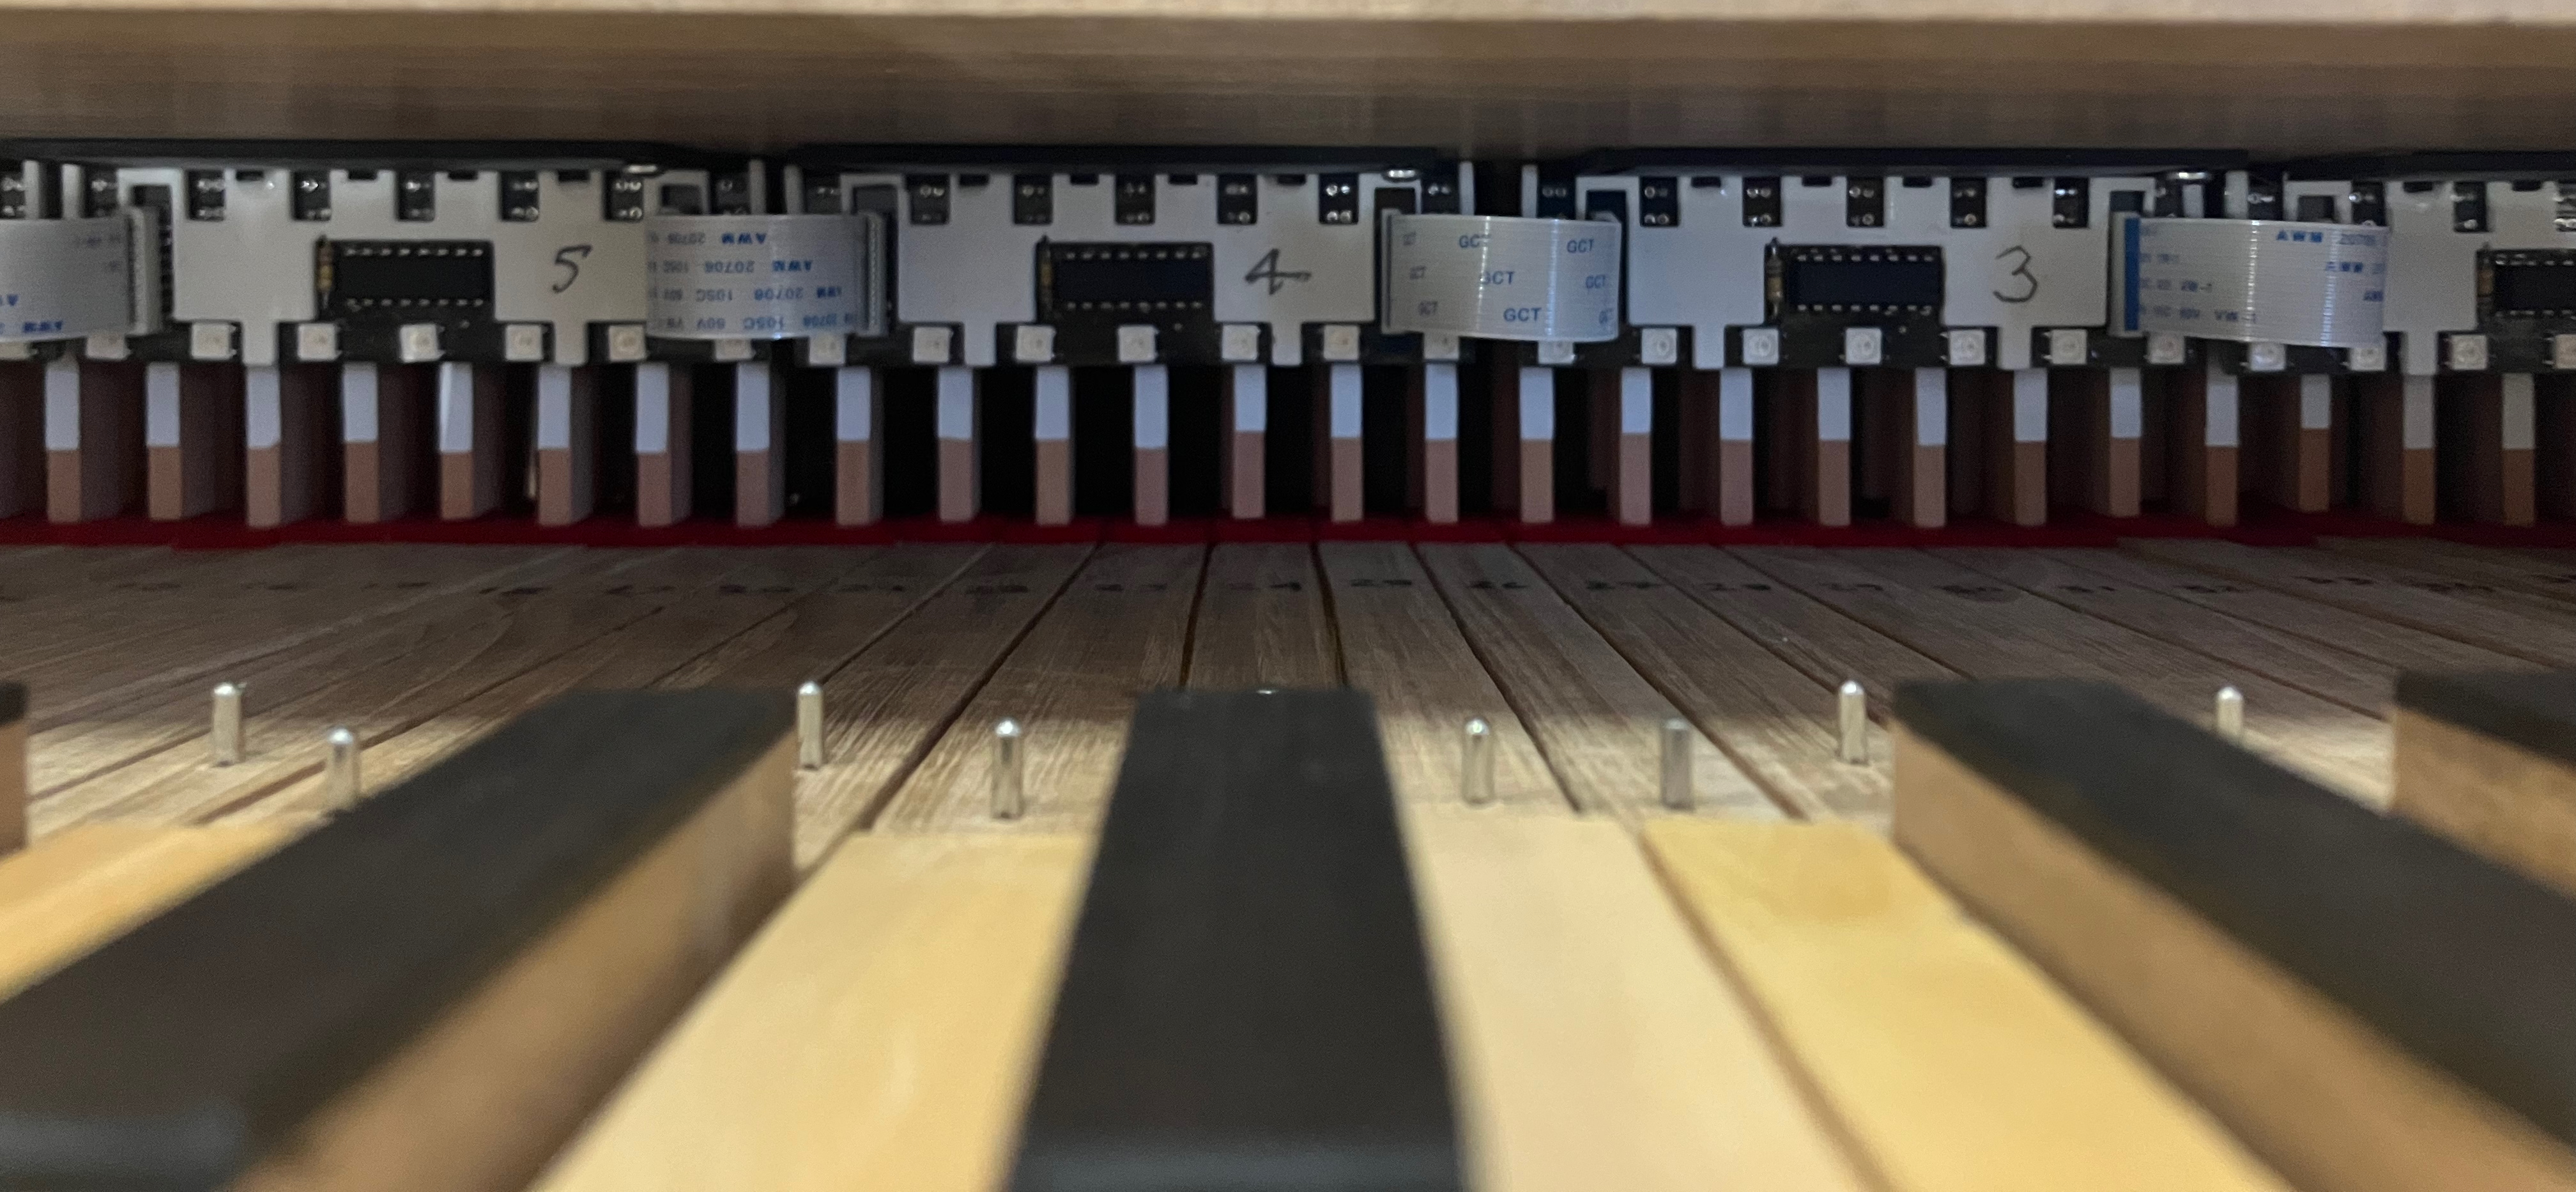
\includegraphics[width=0.7\linewidth,trim={0 0 0 0.5cm},clip]{img/mark-2-front-internal.jpeg}
%   \caption{Inside the Mark 2 interface showing the FFC connecting sensor PCBs together.}
%   \label{fig:internal}
% \end{figure}


\section{Discussion}\label{discussion-interaction}


For haptic keyboard projects, the approach of taking a single key action before expanding to a larger keyboard is an intuitive methodology to use.  The risk with such an approach is the over engineering of concept before expansion takes place. Without losing sight of motivation the project showed that a relatively low-budget, technically simplistic sensor system is enough to enable an interface for interaction. 


For heritage exhibition the temptation to use new technology as a solution to old problems seems a natural one.  Creating an actuated system inspired by an interface was a route to take, but with it comes the inherent risk of getting ``too close'' to the original interface \textcite{michon_hybrid_2018}. The work here builds on the same problem as was being addressed by \textcite{mcalpine_sampling_2014} and how we ``engage those who wish to experience first-hand the musical heritage''. In finding a limitation with the presentation of the interface, \textcite{mcalpine_sampling_2014} naturally looks towards \textcite{gillespie_haptic_1996}. \textcite{mcalpine_sampling_2014} goes on to describe a haptic interface with ``sampled displacement-force curves'', ``linear voice-coil actuators'' for ``real-time force feedback'' and correctly identifies it as ``fundamentally an engineering problem'' but risks in chasing an over engineered solution. 

The specific instruments may be at risk of being lost, but the mechanics are not. We still have access to these systems and means to recreate them without looking necessarily towards a purely technological solution. A modular force feedback system like that of \textcite{cadoz_modular_1990} is certainly an impressive feat, but if a museums collection contains only harpsichords then this pathway is perhaps excessive.

The interface presented here is not complex one and and that is precisely the point. 
Outlined was a process of using replicas of mechanical action and layering the technology on top (or rather behind) in order put the aesthetics at the forefront given the application with the musical heritage domain. This work has incorporated and developed further the ideas of reusing and complimenting the `old' in digital musical instrument design \cite{masu_o-in-nime_2023}. By integrating historical keyboard-building traditions with digital augmentation, the interface offers a possibility to extend the practical lifespan of musical heritage while maintaining the tactile qualities of the original instrument. Rather than prioritising technical novelty, the project demonstrates how digital interventions can support multi-modal interaction with a shared musical heritage, ensuring its continued relevance in contemporary museum contexts.

At the beginning of this chapter \textcite{oboe_mikey_2006} is quoted withe there thoughts on the importance of haptics and problems of its absence in MIDI keyboards and, in particular, how ``sound generation is related only to the key attack velocity and pressure.'' The second comment ``pressure'' is of note. It is unclear when \textcite{oboe_mikey_2006} mentions pressure if it is in relation to purely digital interfaces or acoustic keyboards instruments as well. This may be simply a  reference to aftertouch, which is not present as standard on all digital keyboard interfaces. Key pressure (or after touch) is something that a MIDI keyboard can provide control that an acoustic mechanism cannot. For the interfaces presented here, there is as stream of information potentially available that would enable expressive control, therefore extending the performance techniques and strategies that would otherwise be iunavailable. 

A longer discussion, but one going beyond the scope of this work, is whether the
current setup or its future iterations may be effectively used to build
legitimate replicas of historical musical instruments or even become a kind of
\emph{new} musical instrument altogether. As such, the question is whether these
designs may result in music being practised, performed and recorded with the
instruments. This work supports an overarching narrative extending beyond its
application in museum collections. The NEMUS project
\cite{bologna_nemus_2024}, focusing on developing advanced physical models
simulating the non-linear interaction between subcomponents, has commissioned a
second keyboard to further explore the role of control interfaces in
performance, employing the sense of touch as link between the mechanical world
with the digital, replicating the embodied relationships between performer and
instrument and offering opportunities to modify or even disrupt these
interactions. 

% \textcite{desilvey_curated_2017} puts forward the question ``what could be
% gained if we were to care for the past without pickling it[?]'' If heritage can
% be in a state of living -- and conservation approach is akin to `dead`
% \cite{poulios_moving_2010} -- then there must also be a transition phase where
% heritage dies and moves from one state to the other. Rather than resisting and
% fearing this transition, \textcite{desilvey_curated_2017} suggests that we might
% rather embrace this natural event. \textcite[p. 75]{barclay_preservation_2005}
% touches on this same idea as he discusses `benign neglect' where the
% preservation of playing state --or Currency-- is passive but the decision to do
% so is very deliberate. We might then toward other approaches to maintaining the
% idea of an instrument. Rather than striving for the ``Exact copy'' we instead
% can consciously and deliberately seek an `imperfect' that elicits the
% ``exploring the social, political, historical, conceptual, contextual'' aspects
% of musical instrument heritage \cite{holzer_imperfect_2025}.

% This study has presented the design and implementation of an electronically
% augmented keyboard for the Tagliavini Collection at the San Colombano Museum.
% By leveraging optical sensors and MIDI-controlled sample libraries, the
% keyboard allows users to explore a harpsichord's sonic and mechanical essence
% without compromising the integrity of the museum's historical artefacts.
% Preliminary feedback shows that the keyboard has the potential to enhance the
% museum experience, particularly for those unfamiliar with early keyboard
% instruments. However, technical limitations, such as calibration
% inconsistencies and restrictions imposed by the commercial sample library,
% highlight opportunities for refinement. These issues will be addressed in
% future iterations, including a second keyboard designed to control advanced
% physical models. This work opens new possibilities for engaging with heritage
% collections while respecting their authenticity. It also serves as a
% foundation for further research projects exploring embodied cognition in
% historical instruments, and it may provide a useful framework to investigate
% the links between physical modelling and digital musical interface design.

% \section{Main Points}

% \begin{itemize}
%     \item Reintroduction of physical interaction with historical instrument
%     \item modularity of the process for further application (design methodology)
%     \item implications for musical instrument museum exhibition (curated decay
%     and living heritage;)
%     \item open sourcing and software sustainability methodology applied to
%     hardware (cad, firmware measurements)
%     \item Accessibility of projects of this kind
% \end{itemize}

% \begin{itemize}
%     \item context in thesis
%     \item context in wider work
%     \item development process
%     \item technical details
%     \item deployment and lessons learned
% \end{itemize}